\documentclass[conference, dvipsnames]{IEEEtran}

% Usepackages
\usepackage{cite}
% provides various features to facilitate writing math formulas and to improve the typographical quality of their output.
\usepackage{amsmath}
% \usepackage[cmex10]{amsmath}
\interdisplaylinepenalty=2500
\usepackage{amssymb,amsfonts}
\usepackage{algorithmic}
\usepackage{graphicx}
% \usepackage{graphicx}
\usepackage{textcomp}
\usepackage{xcolor}

% formatting from IEEE conference. Needs to be fitted with our natbib
\def\BibTeX{{\rm B\kern-.05em{\sc i\kern-.025em b}\kern-.08em
		T\kern-.1667em\lower.7ex\hbox{E}\kern-.125emX}}

%%%%%%%%%%%%%%%%%%%%%%%%
%Article stuff
%%%%%%%%%%%%%%%%%%%%%%%%
% This package serves to balance the column lengths on the last page of the document.
% please, insert \balance command in the left column of the last page
\usepackage{balance}
\usepackage{supertabular}
\usepackage{paralist}
\usepackage{booktabs}

%% to enable \thank command
\IEEEoverridecommandlockouts 
% to typeset algorithms
\usepackage{algorithm}
%\usepackage{algpseudocode}
% to typeset code fragments
\usepackage{listings}
% to make an accent \k be available
\usepackage[T1]{fontenc}
% por urls typesetting and breaking
\usepackage{url}
% for vertical merging table cells
\usepackage{multirow}
\usepackage{siunitx}


%%%%%%%%%%%%%%%%%%%%%%%%
%Mixed packages
%%%%%%%%%%%%%%%%%%%%%%%%
\usepackage[hidelinks]{hyperref}
\usepackage{graphicx}
\usepackage[textsize=scriptsize]{todonotes}
\usepackage{glossaries}
\usepackage[numbers]{natbib}
\usepackage{subcaption}
\bibliographystyle{plainnat}

\let\labelindent\relax %Needed before enumitem to avoid error with IEEE template
\usepackage{enumitem}
% Encoding %
\usepackage[utf8]{inputenc}
\usepackage{enumitem}
\usepackage{framed}


%%%%%%%%%%%%%%%%%%%%%%%%
%Figures
%%%%%%%%%%%%%%%%%%%%%%%%

\usepackage{tikz}
\usepackage{pgfplots}

% Tables %
\usepackage{tabularx}
\usepackage{xltabular}
\newcolumntype{Y}{>{\centering\arraybackslash}X}
\usepackage{booktabs} % for professional tables
\usepackage{tikz}
\usetikzlibrary{positioning}
\usepackage{longtable}
\usepackage{makecell}
\usetikzlibrary{shapes.geometric, arrows}
\usetikzlibrary{matrix,positioning,arrows.meta,arrows}

\tikzset{my arrow/.style={-latex},
	set@com@col/.style={},set@com@col@aryarg/.style={column #1/.style={set@com@col}},
	set@com@row/.style={},set@com@row@aryarg/.style={row #1/.style={set@com@row}},
	set common column/.style 2 args={set@com@col/.style={#2}, set@com@col@aryarg/.list={#1}},
	set common row/.style 2 args={set@com@row/.style={#2}, set@com@row@aryarg/.list={#1}},
}

%%%%%%%%%%%%%%%%%%%%%%%%
%Defines
%%%%%%%%%%%%%%%%%%%%%%%%

\newtheorem{definition}{\textbf{Definition}}

% Autoref
\def\sectionautorefname{Section}
\def\subsectionautorefname{Section}
\def\subsubsectionautorefname{Section}
\def\figureautorefname{Fig.}
\def\definitionautorefname{Definition}

% Plates
\usepackage{amstext}
\usepackage{tikz}
\usetikzlibrary{arrows,decorations.pathmorphing,fit,positioning}

\newcommand{\dir}{\text{Dirichlet}}
\newcommand{\mult}{\text{Multinomial}}


% Macros
%%%%%%%%%%%%%%%%%%%%- Commands -%%%%%%%%%%%%%%%%%%%%%%%%%%%%%
\newcommand{\langballe}[2][]{\todo[color = cyan, #1]{\textbf{Langballe:} #2}}
\newcommand{\vejleder}[2][]{\todo[color = magenta, #1]{\textbf{Vejleder:} #2}}
\newcommand{\simba}[2][]{\todo[color = green, #1]{\textbf{Simba:} #2}}
\newcommand{\dennis}[2][]{\todo[color = pink, #1]{\textbf{Dennis:} #2}}


% Glossaries
\newacronym{lda}{LDA}{latent Dirichlet allocation}
\newacronym{NLP}{NLP}{Natural Language Processing}
\newacronym{tf-idf}{tf-idf}{Term Frequency-Inverse Document Frequency}
\newacronym{lm}{LM}{Language Model}
\newacronym{vi}{VI}{Variational Inference}
\newacronym{pr}{PR}{PageRank}
\newacronym{ppr}{PPR}{Personalized PageRank}
\newacronym{bm25}{BM25}{Okapi Best Matching 25}
\newacronym{ir}{IR}{Information Retrieval}
\newacronym{map}{MAP}{Mean Average Precision}
\newacronym{dag}{DAG}{Directed Acyclic Graph}

%Glossary changes
%%%%%%%%%%%%%%%%%%%%%%%%
% Switch off hyperlinks for all uses of \gls etc.
% Hyperlinks will be inserted manually in the custom display style
\setkeys{glslink}{hyper=false}

\renewcommand*{\CustomAcronymFields}{%
	name={\the\glsshorttok},%
	description={\the\glslongtok},%
}

\renewcommand*{\SetCustomDisplayStyle}[1]{%
	\defglsentryfmt[#1]{%
		\ifdefempty\glscustomtext
		{%
			\ifglsused\glslabel
			{% subsequent use
				% Assuming all acronyms are written in upper case, so
				% not bother to check for case changes.
				\glsifplural
				{% subsequent use, plural
					\glshyperlink[\glsentryshortpl{\glslabel}]{\glslabel}%
				}%
				{% subsequent use, singular
					\glshyperlink[\glsentryshort{\glslabel}]{\glslabel}%
				}%
			}%
			{% first use
				\glsifplural
				{% first use, plural
					\glscapscase
					{% no case change
						\glstarget{\glslabel}{\glsentrylongpl{\glslabel}\glsinsert}%
						\space(\glsentryshortpl{\glslabel})%
					}%
					{% first letter upper case
						\glstarget{\glslabel}{\Glsentrylongpl{\glslabel}\glsinsert}%
						\space(\glsentryshortpl{\glslabel})%
					}%
					{% all caps
						\glstarget{\glslabel}{\MakeTextUppercase{%
								\glsentrylongpl{\glslabel}\glsinsert}}%
						\MakeTextUppercase{\space(\glsentryshortpl{\glslabel})}%
					}%
				}%
				{% first use, singular
					\glscapscase
					{% no case change
						\glstarget{\glslabel}{\glsentrylong{\glslabel}\glsinsert}%
						\space(\glsentryshort{\glslabel})%
					}%
					{% first letter upper case
						\glstarget{\glslabel}{\Glsentrylong{\glslabel}\glsinsert}%
						\space(\glsentryshort{\glslabel})%
					}%
					{% all caps
						\glstarget{\glslabel}{\MakeTextUppercase{%
								\glsentrylong{\glslabel}\glsinsert}}%
						\MakeTextUppercase{\space(\glsentryshort{\glslabel})}%
					}%
				}%
			}%
		}%
		{% \glsdisp used
			\ifglsused\glslabel
			{% subsequent use
				\glshyperlink[\glscustomtext]{\glslabel}%
			}%
			{% first use
				\glstarget{\glslabel}{\glscustomtext}%
			}%
		}%
	}%
}

\SetCustomStyle



\begin{document}
% Autoref
\def\sectionautorefname{Section}
\def\subsectionautorefname{Section}
\def\subsubsectionautorefname{Section}
%\def\figureautorefname{Fig.}
\def\definitionautorefname{Definition}

\section*{Summary}
\todo[inline]{Update text later depending on what changes we make to the paper}
%introduction
News is being broadcast every day around the world in the form of news articles, television, and newspapers, which supply people with the latest information.
Searching and categorizing the news is becoming a bigger problem since news is created at all times.
Topic modeling is an approach that takes a set of documents and generates topics that can be used for categorizing text.
We specifically look at extending the \gls{lda} model and the \gls{pam} with metadata.

In this paper we answer these research questions:
\begin{itemize}
	\item \textit{How can we establish models that incorporate metadata from the Nordjyske dataset?}
	\item \textit{How does including metadata within such models impact the resulting topics?}
\end{itemize}

%dataset
We work with a dataset Nordjyske, a Danish news agency.
This dataset contains $248,385$ articles from 2017 to 2019.
Basic preprocessing is done to make the data more applicable for topic models.
Each article includes three types of metadata: author, category, and taxonomy, that we chose to extend our topic models with.

The author field is for the author who has written the article.
This field is fully observed within the dataset, and each article only has a single author, so we do not account for multiple authors.
There are $227$ different authors within the dataset and after preprocessing $184$ remain.

The category field describes a variety of different aspects, but the categories are generally either about a specific newspaper or an overall subject.
This field is also fully observed within the dataset, and there are $58$ unique categories in the dataset before processing, and $34$ categories after preprocessing.

The taxonomy field describes a hierarchical sequence of the topical or geographical subject of the articles.
Each sequence consists of several taxonomy entries.
This field is only partially observed within the dataset, with ${\sim}25\%$ of the articles containing this field.
There are $1135$ different taxonomies and after preprocessing $345$ remain.

%models
The models we have made that include metadata for our evaluations are called the author-topic, category-topic, and taxonomy-topic model.
We also use a standard \gls{lda} model as a baseline for the performance of our models.
In \gls{lda}, $D$ is the number of documents in the corpus, $N_d$ is the number of words in document $d$, and $K$ is the number of topics.
Topics are represented as distributions over words and documents are represented as distributions of topics.

In the author-topic and category-topic models, there are no document-topic distributions $\theta$.
Instead, each of the $A$ authors and $C$ categories have their own topic distribution.
This is based on the assumption that authors prefer to write about specific topics and that categories of the articles were chosen based on the content of the finished article or that local newspapers have their own unique topic preferences.
For our category-topic model and author-topic model, each document $d$ is associated with one category $c_d$ from a set of categories $C$ and one author $a_d$ from a set of authors $A$, which is used when drawing a word topic.

To have our taxonomy-topic model handle the hierarchical structure of the taxonomy metadata field, we use a hierarchical topic model called the \acrfull{pam}.
Pachinko allocation generalizes \gls{lda}, making it possible to construct topic hierarchies based on any \gls{dag} structure.
\gls{pam} is a topic model focusing on finding topics of different abstraction levels and modeling the correlations between these topics.
Without modification, \gls{pam} finds topics with the same structure as our taxonomy, but the taxonomy values would be disregarded during training since it would generate new taxonomy sequences.
However, in our case, we have a dataset with a partially observed taxonomy field (${\sim}25\%$ of the documents), and we want to use the existing metadata information to estimate the topics quicker and more accurately.
To account for this, we only sample the unobserved nodes within the topic sequences.
For some of the dataset only the fourth layer is unobserved, but for the ${\sim}75\%$ documents without a taxonomy sequence, all layers are unobserved.
The observed taxonomy sequences are never sampled, hence they are 'locked' in place.
This creates a constant context for the taxonomy topics, which the documents with unobserved taxonomy sequences are fitted around.

%evaluation
The main metric used, in this experiment, is the topic coherence metric.
This metric indicates how semantically similar the top words within each topic are, and is an indication of the quality of the topics of a topic model.
The second metric used in the experiment is topic difference.
The topic difference is another metric that is used to check the quality of the topic model.
It is based on the assumption that a good topic model has little overlap between topics.

Before fitting our models, we search for the optimal hyperparameters for our models, since these can vary based on the dataset.
The hyperparameters we are testing in this grid search are the number of topics $K$ and an $\alpha$ and $\eta$ parameter.
We only run the grid search on the standard \gls{lda} model, with the assumption that the number of topics that perform well for this model, also performs well for the metadata models, when the same dataset is used.
Based on the topic coherence of the model we choose $K = 90$, $\alpha = 0.01$, and $\eta = 0.1$ as the hyperparameters for all models in the experiment.

For the results, the topic coherence of \gls{lda} is 0.520, author-topic is 0.335, category-topic is 0.370, and taxonomy-topic is 0.660.
This shows that the Author and Category-Topic models performed the worst in topic coherence, whereas the Taxonomy-Topic model is outperforming all other models.
However, the run time of the Taxonomy model is much higher than the standard \gls{lda}.

%discussion
In the analysis of the models, we explored the highest probable words from each model, except the taxonomy-topic model, that would appear in a chosen article.
It is seen that there is a large amount of overlap between the models, but the words that best summarized the article came from the \gls{lda} model.

For the author-topic and category-topic models, we are also able to analyze the similarity between author pairs and category pairs.
This similarity is calculated with the symmetric Kullback-Leibler divergence of either the author-topic distributions or the category-topic distributions.
This gives the intuition of how similar authors are based on the topics they write, and categories in the topics they cover.
It is seen that it is difficult to find specifically why authors are similar because they often write about many different subjects.
From the category similarities, there are obvious high similarity pairs, such as 'Sport-avis' and 'Morsø Sport' where they both include sports articles.

For the taxonomy-topic model, it was found that the topics, in general, were the most understandable of all topic models, which made sense with it having the highest topic coherence.
The taxonomy-topic model was also able to separate words without meaning into their own topics, which allows the model to apply an extra layer of preprocessing, automatically filtering away irrelevant words into topics


%appendix
As further experimentation and exploration, we tested what would happen if we did further preprocessing.
We also tested the effect of including multiple topic distributions in our models and what would happen if we used the author and category metadata in the \gls{pam}.

For further preprocessing, we tested what effect including stemming in our dataset would have on the models.
With stemming on the \gls{lda} model, it was seen that there were a lot fewer unique words.
When looking at the topics of the model, it was seen that they generally did not change much, but may be slightly more understandable with fewer words with the same meaning.

One of the new models we made is called the author-category model.
This model includes both an author-topic distribution and a category-topic distribution and uses both to draw word topics.
This model has only a slightly higher topic coherence of 0.390 compared to the author-topic and category-topic model, and the topics are still not very understandable.

We also made two other models called Author-Doc and Category-Doc.
These models are made by combining the \gls{lda} model with the author-topic and category-topic mode, and also use both distributions to draw word topics.
We run these models using the same hyperparameters as all the other models and they get similar results to the standard \gls{lda} model.
Author-doc gets a topic coherence of 0.543 and category-doc gets 0.530.

Finally, we tested what would happen if we ran \gls{pam} with just the author and category metadata.
A four-layer \gls{pam} was used for both of these models, but otherwise, the same structure is used as with the taxonomy-topic model.
The author \gls{pam} gets a topic coherence of 0.598 and the category \gls{pam} gets 0.585.
These models achieved better results than the previous author and category models and the \gls{lda} model but had lower topic coherence compared to the taxonomy-topic model.

\glsresetall

\title{Integrating News Article Metadata into Topic Models\\
%\thanks{Identify applicable funding agency here. If none, delete this.}
}

%\IEEEauthorblockN{Dennis Højbjerg Rose, Peter Langballe Erichsen, and Rasmus Engesgaard Christensen}\\
%\IEEEauthorblockA{Department of Computer Science, Aalborg University,\\Selma Lagerløfs Vej 300, 9220 Aalborg Øst, Denmark\\Email: \{drose16, perich16, rech16\}@student.aau.dk}}

\author{
\IEEEauthorblockN{Dennis Højbjerg Rose}
\IEEEauthorblockA{\textit{Department of Computer Science} \\
\textit{Aalborg University}\\
Aalborg, Denmark \\
drose16@student.aau.dk}
\and
\IEEEauthorblockN{Peter Langballe Erichsen}
\IEEEauthorblockA{\textit{Department of Computer Science} \\
\textit{Aalborg University}\\
Aalborg, Denmark \\
perich16@student.aau.dk}
\and
\IEEEauthorblockN{Rasmus Engesgaard Christensen}
\IEEEauthorblockA{\textit{Department of Computer Science} \\
\textit{Aalborg University}\\
Aalborg, Denmark \\
rech16@student.aau.dk}
}

\maketitle

\begin{abstract}
	We introduce two topic models that extend \gls{lda} to include author and category metadata information and a third model which applies taxonomy metadata on the \gls{pam}.
The author-topic and category-topic models are based on the author-topic model from \citet{author_topic_2012} with slight modifications, and the taxonomy-topic model uses the \gls{pam} from \citet{li2006pachinko}.
To make the \gls{pam} include the metadata information in each layer of its \gls{dag} structure, a novel topic locking mechanism is created.
The results show that while, for the applied dataset, the author-topic and category-topic models get a lower topic coherence than \gls{lda}, the taxonomy-topic model has the highest topic coherence and most understandable topics.
For each model, we also give proposals for how they can be used for recommendation in a news article environment.
\end{abstract}

\glsresetall

\begin{IEEEkeywords}
	component, formatting, style, styling, insert
\end{IEEEkeywords}
\todo[inline]{Find keywords. IEEE approved keywords can be found at: \url{https://ieeecs-media.computer.org/assets/pdf/taxonomy.pdf}}
\glsresetall

\todo[inline]{reference the appendix more in the paper}
% - Introduction (7.5 \%) 
\section{Introduction}\label{sec:introduction}
% Intro to meta data
Data is everywhere and it is used in many different scenarios and use cases. 
When referring to a data set, we talk about data having meta-data information or attributes, which are the entries that could describe certain features about the data, like petal length from well-known IRIS data set\footnote{https://archive.ics.uci.edu/ml/datasets/iris} describing the length of a particular flower's petals.
However, there is usually a lot of data, that is not used, either because it is not useful or we do not know how to use it properly.

% LDA / Topic Modeling Intro
Within the field of topic modeling, the goal is to find underlying topics within a certain data set.
These topics are constructed based on the text documents in the dataset and words within these documents. 
Other extensions of \gls{lda} have also modeled various other information to generate better topics and/or topics with different focuses and potential uses.

% Author-Topic
One of the well-known extensions is the Author-Topic model by \citet{author_topic_2012} that combines the \gls{lda} model with author information to model the relationship between authors and the documents, which they have written.
This is based on the assumption that most authors usually write about only a few different topics.
By modeling this relationship, they find connections between authors and topics, and between different authors, giving more underlying information to the topics.
They also show that the Author-Topic combination yields better and more coherent topics, which begs the question of whether any other document-related data can be applied similarly.

% Topic Modeling dataset
In \gls{lda}, the data used is a corpus of documents, with each document containing a sequence of words.
However, the dataset that will form this corpus also often includes various other data than just the text within the documents, such as authors, time of publishing, tags, etc.
% Metadata definition
We define this other data as metadata, that is data related to the documents in the corpus, but not directly a part of the text.
In most models, metadata is not used.
However, there is some previous work that attempts to make full use of the dataset available by incorporating various metadata into topic models.

% In this paper
In this paper, we will be taking a closer look at a specific dataset and construct different topic models that incorporate various metadata.
We do this in order to see if they can improve the quality of the topics or the efficiency of the model.
We will also investigate the differences between the produced topics for various models, and evaluate their potential uses.

We will be using a dataset from Nordjyske, a danish news agency that maintains multiple local newspapers throughout the North Jutland region.
We will construct topic models that account for the specific metadata available within this dataset.
This metadata includes author information, as well as higher-level categorical information, which will be described in \autoref{sec:dataset}.

% Problem Statement
With these areas of focus, we can define the problem we investigate:

\begin{itemize}
	\item \textit{How does including metadata within the \gls{lda} model impact the resulting topics?}
	\item \textit{How can multiple metadata fields be integrated within a topic model?}
\end{itemize}

Our work is similar to that of \citet{MetaLDA2017} since we work with meta information and are applying it to an \gls{lda} model.
However, \citet{MetaLDA2017} learn a specific Dirichlet prior based on the meta-information given in their dataset, which gives a specific topic distribution for each meta-information field and in turn affect the document-topic distribution used with the \gls{lda}.
Instead of using the document-topic distribution for drawing word topics, we want to create a new meta-topic distribution which influences the drawn topics.
An example is the author-topic model from \citet{author_topic_2012}, where they also create a distribution for each author.
We would like to see what happens when you create a meta-topic distribution for any specific meta-information, such as the author information, and see how it affects the resulting topics.
The intuition behind this is to create new topic models, which describe the data in a different way using topics that are influenced by metadata.
For example, if the metadata describes something about geographic locations, location-specific topics will be generated.

\todo[inline]{Possibilities for adding more to the section: write more about our specific approach, still on overview/abstract level. Write a little after the problem statement about what the questions cover/will give.}

% Paper Structure
The paper is organized as follows:
In \autoref{sec:related_work}, we explore articles related to topic modeling and topic models using metadata.
\autoref{sec:overview} gives an overview of our method by separating the process into steps.
\autoref{sec:dataset} describes the dataset used in the experiments.
In \autoref{sec:plate_notation}, \gls{lda}, the metadata topic models, and the model combinations are described, and their plate notation is shown.
In \autoref{sec:experiment}, we set up an experiment to test the performance of the different metadata topic models along with their combinations and present the results.
In \autoref{sec:discussion}, we analyze and discuss the results of our experiment.
Finally, in \autoref{sec:conclusion}, conclusions and future work are given.
\todo[inline]{Update paper structure}

%

%
%% - Preliminaries/"Experiment" (20 \%)
%%		- Data
%%		- Setup
%%		- Analysis


\section{Dataset}
Nordjyske is a Danish news agency that maintains multiple newspapers, radios and other news sources throughout north Jutland, a region in Denmark.
They store their news articles in a non-public database, where each article contains multiple meta-data fields which describes some aspect of the data eg. author.
The dataset is from 2017 to 2019 and contains 139261 articles which uses a vocabulary of 69192 unique words.
One of the metadata fields is the Category field, which both describes where the article is supposed to be located(within a newspaper) and also which subject the article is about.
These meta-data are very interesting in that they detail the data in certain ways which might be useful in some way.

In the following section, we describe each of the meta-data fields which are analysed.

\subsection{Author}
This field mentions the author, who have written the article.
Each article only has a single author, so we do not account for multiple authors in this paper.
This field is fully observed within the dataset, which means that every article has an author.
There are $227$ different authors within the dataset and they are almost evenly distributed in the number of articles they have written.

\subsection{Category}
The category field describes a variety of different aspects. 
This field is fully observed within the dataset and there are $58$ different categories.
A proportion of the articles contains which specific newspaper, they belong to, eg. Aalborg-Newspaper.
Another proportion of the category fields describes the overall theme, such as Culture and Sports-newspaper.

\subsection{Taxonomy}
The taxonomy field describes a hierarchical structure of the topical or geographical subject of the articles.
This field is only partially observed within the dataset, which means that roughly $50\%$ of the articles contain this field.
We observe a general pattern when traversing this field which is:
\begin{itemize}
	\item Places/Country/Region/Town
	\item Topics/Sub-Topic/Subsub-topic
\end{itemize}
Examples of this field are:
\begin{itemize}
	\item PLACES/Danmark/Nordjylland/Aalborg/Lillevorde
	\item TOPICS/Religion/Christianity
\end{itemize}

%% - Related works (7.5 \%))
\section{Related Work}\label{sec:related_work}

\citet{mimno2008topic} describes two general topic model patterns, called ''upstream`` and ''downstream`` topic models.
These patterns describe how metadata is incorporated in topic models.
In the downstream pattern, metadata is incorporated in the model by having the topic model generate both the words and the metadata simultaneously.
Here each topic has a distribution over words, as well as a distribution over metadata values.
In the upstream pattern, the topic model is conditioned on metadata elements by representing document-topic distributions as element specific distributions.
This way the model learns assignments of the words in each document to the metadata.

\citet{author_topic_2012} have developed a \gls{lda} model called the Author-Topic model, which incorporates authorship information in the \gls{lda} model.
Specifically, each document has a vector of authors, where for each word an author is drawn from this vector.
The author is then used in combination with an author-topic distribution to draw a specific topic that this author writes about.
The words from the topic-word distribution can be generated based on this topic.
The purpose of using authorship information in this way, is to show patterns in which topics an author usually writes about, and be able to explore how related authors are in what they write about.
\citeauthor{author_topic_2012} also show that the combination of authorship and \gls{lda} yield more coherent topics.


\citet{MetaLDA2017} presents a recent model which can incorporate both metadata information and word embeddings within a topic model.
Since the field of incorporating word embeddings within generative topic models have gained popularity\cite{dieng2020topic}, \citet{MetaLDA2017} show how to use this information for a variety of different datasets.
They also compare against a list of other models that take either metadata information or word embeddings into account when doing inference.


\citet{tea_leaves} is a well-known paper within the topic modeling community, which presents different methods for evaluating probabilistic topic models. 
An important observation they made, is that a good held-out likelihood, normally called perplexity, infers less semantically meaningful topics.
They also present two different human judgment methods, which can be used to evaluate topic models.
\citet{topic_coherence_2015} introduce new measures for evaluating topic models, where some of them use the co-occurrence or conditional probability of words within topics to measure how coherent the topics are. 
In order to verify that these metrics work, they conduct a large user study in conjunction with these metric evaluations.


\citet{li2006pachinko} present a \gls{dag} structured topic model, called the \acrfull{pam}, where topics are in a hierarchical structure, which allows it to find two types of topics, namely super-topics and sub-topics. 


\citet{card2017neural} describe how to incorporate metadata information within a neural network to find topics using variational inference methods.

From these works, we mainly use the concepts from \citet{author_topic_2012} for how we use metadata in our models, though with slight changes in the models for handling the characteristics of our data.


\section{Preliminaries}\label{sec:preliminaries}
Here we present the foundation for the two models that we are adapting in this paper.

\subsection{\Acrlong{lda}}
The purpose of \gls{lda}, and topic models in general, is to create a tool for exploring collections of text.
Topic models do this by uncovering the underlying semantic structure of a text collection by using hierarchical Bayesian models.
\Gls{lda} uncovers this semantic structure by discovering patterns of word use in documents and finding topics based on these~\cite{blei2009topic}.

The standard \gls{lda} by \citet{blei2003latent} can be described by the following generative process, which is the way the model assumes the documents arose:
$D$ is the number of documents in the corpus, $N_d$ is the number of words in document $d$, $V$ is the size of the vocabulary, and $K$ is the number of topics.
Topics are represented as distributions over words and documents are represented as distributions over topics.
\Gls{lda} assumes that the topics are shared across the corpus, while the document-topic distributions are unique for each document.
For each topic $k \in \{1,\dots, K\}$ a topic-word distribution $\beta_k$ is sampled from a V-dimensional Dirichlet distribution parameterized by $\eta$.
That is, K topics $\beta_{1:k}$ are sampled, each being a distribution over the vocabulary, written as: $\beta_k \sim Dirichlet(\eta)$.
Likewise, for each document $d \in \{1,\dots, D\}$ a document-topic distribution $\theta_d$ is sampled from a K-dimensional Dirichlet distribution parameterized by $\alpha$.
For each word $n \in \{1, \dots, N_d\}$ in each document $d$, a topic $z_{d,n}$ is sampled from a K-multinomial distribution $\theta_d$, and then a word $w_{d,n}$ is sampled from a V-multinomial distribution $\beta_{z_{d,n}}$.
The generative process for each document is seen in these steps:

\vspace{\topsep}
\begin{enumerate}
	\item Draw topic proportion $\theta_d \sim Dirichlet(\alpha)$
	\item For each word $n$ in the document:
	\begin{enumerate}
		\item Draw topic assignment $z_{d,n} \sim Mult(\theta_d)$
		\item Draw word $w_{d,n} \sim Mult(\beta_{z_{d,n}})$
	\end{enumerate}
\end{enumerate}
\vspace{\topsep}

The result is $K$ topics, based on $D$ documents.
These topics are represented by a $K \times V$ matrix of topic-word distributions and a $D \times K$ matrix of document-topic distributions.
The plate notation for \gls{lda} can be seen in \autoref{fig:standard_lda}.

\begin{figure}[h]
  \centering
  \resizebox{\columnwidth}{!}{%
	  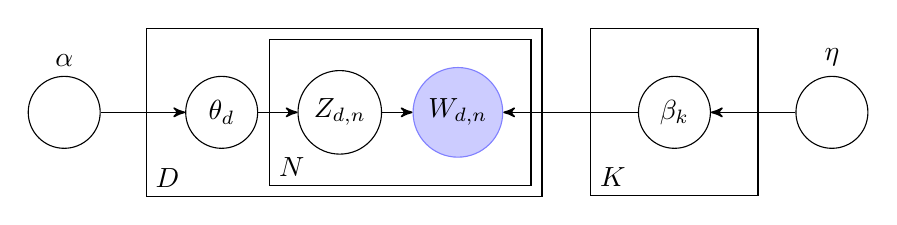
\begin{tikzpicture}
	    [
	      observed/.style={minimum size=15pt,circle,draw=blue!50,fill=blue!20},
	      unobserved/.style={minimum size=26pt,circle,draw},
	      post/.style={->,>=stealth',semithick},
	    ]
	
	    \node (w-j) [observed] at (0,0) {$W_{d,n}$};
	    \node (z-j) [unobserved] at (-1.5,0) {$Z_{d,n}$};
	    \node (theta) [unobserved] at (-3,0) {$\theta_d$};
	    \node (alpha-hyper) [unobserved, label=above:$\alpha$,left of=theta, node distance=2cm] {};
	    \node (beta-hyper) [unobserved] at (2.75,0) {$\beta_k$};
	    \node (eta-hyper) [unobserved, label=above:$\eta$, ,right of=beta-hyper, node distance=2cm] {};
	    
	    \path
	    (z-j) edge [post] (w-j)
	    (alpha-hyper) edge [post] (theta)
	    (theta) edge [post] (z-j)
	    (beta-hyper) edge [post] (w-j)
	    (eta-hyper) edge [post] (beta-hyper)
	    ;
	    
	    \node [draw,fit=(w-j) (theta), inner sep=14pt] (plate-context) {};
	    \node [above right] at (plate-context.south west) {$D$};
	    \node [draw,fit=(w-j) (z-j), inner sep=10pt] (plate-token) {};
	    \node [above right] at (plate-token.south west) {$N$};
	    \node [draw,fit=(beta-hyper) (beta-hyper), inner sep=17pt] (plate-context) {};
	    \node [above right] at (plate-context.south west) {$K$};
	  \end{tikzpicture}
  }
	\caption{Plate notation for \gls{lda}.}
	\label{fig:standard_lda}
\end{figure}



\subsection{Author-topic \gls{lda}}\label{subsec:auth_prelim} \vejleder{introducer modellen som den er i \cite{author_topic_2012}, gerne flere detaljer}
\citet{author_topic_2012} present the author-topic model.
It seeks to find topics based on author metadata, and is based on the assumption that authors prefer to write about specific topics.
In this model, there are no document-topic distributions $\theta$, but rather one author-topic distribution for each author.
The reason for this is to find the interest of authors within the documents that we are analyzing.
The generative process for the author-topic model is similar to that of the \gls{lda} model with a few minor changes.
The model assumes that there are multiple authors for each document which is modeled by the $\boldsymbol{a_d}$ and $x$ variables in \autoref{fig:original_author_lda}.
Before drawing a word topic, we need to select an author $x$ from $\boldsymbol{a_d}$.
The generative process is seen in the following steps:
\vspace{\topsep}
\begin{enumerate}
	\item For each author, draw topic proportion $\theta_a \sim Dirichlet(\alpha)$
	\item For each word $n$ in the document:
	\begin{enumerate}
		\item Draw author assignment $x \sim U(\boldsymbol{a_d})$
		\item Draw topic assignment $z_{d,n} \sim Mult(\theta_x)$
		\item Draw word $w_{d,n} \sim Mult(\beta_{z_{d,n}})$
	\end{enumerate}
\end{enumerate}
\vspace{\topsep}
Here $U()$ denotes the discrete uniform distribution.

\citet{author_topic_2012} describe the author-topic model where for each document $d$, they assign a vector of authors $a_d$ from a set of authors $A$, and for each word uniformly choose an author $x$ at random from this vector.
The original plate notation for the author-topic model can be seen in \autoref{fig:metadata_lda}.

\begin{figure*}[ht]
	\centering
	\begin{subfigure}{0.275\textwidth}
		\centering
		\resizebox{\textwidth}{!}{%
			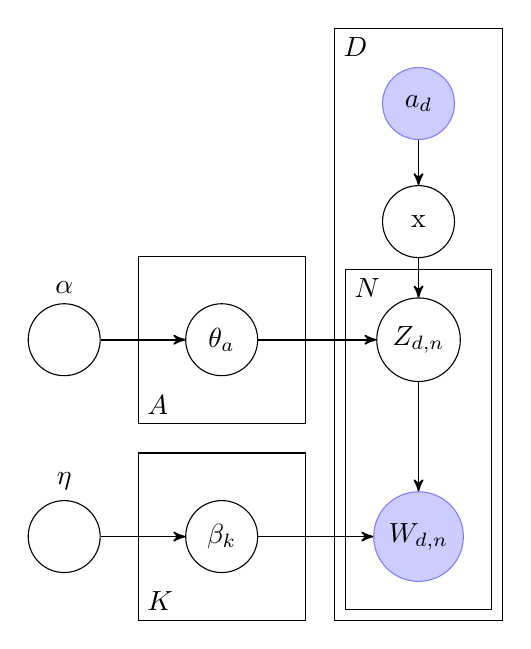
\begin{tikzpicture}
	[
	observed/.style={minimum size=26pt,circle,draw=blue!50,fill=blue!20},
	unobserved/.style={minimum size=26pt,circle,draw},
	post/.style={->,>=stealth',semithick},
	]
	
	\node (w-j) [observed] at (0,0) {$W_{d,n}$};
	\node (z-j) [unobserved, above of= w-j, node distance=2.5cm] {$Z_{d,n}$};
	\node (x) [unobserved, above of=z-j, node distance=1.5cm] {x};
	\node (author_obs) [observed, above of= x, node distance=1.5cm] {$a_d$};
	\node (author_dist) [unobserved, left of=z-j, node distance=2.5cm] {$\theta_a$};
	\node (alpha-hyper) [unobserved, label=above:$\alpha$, left of=author_dist, node distance=2cm] {};
	\node (beta-hyper) [unobserved, left of = w-j, node distance=2.5cm] {$\beta_k$};
	\node (eta-hyper) [unobserved, label=above:$\eta$, left of=beta-hyper, node distance=2cm] {};
	
	\path
	(z-j) edge [post] (w-j)
	(alpha-hyper) edge [post] (author_dist)
	(author_obs) edge [post] (x)
	(x) edge [post] (z-j)
	(author_dist) edge [post] (z-j)
	(beta-hyper) edge [post] (w-j)
	(eta-hyper) edge [post] (beta-hyper)
	;
	
	\node [draw,fit=(w-j) (author_obs), inner sep=14pt] (plate-context) {};
	\node [below right] at (plate-context.north west) {$D$};
	
	\node [draw,fit=(w-j) (z-j), inner sep=10pt] (plate-token) {};
	\node [below right] at (plate-token.north west) {$N$};
	
	\node [draw,fit=(beta-hyper) (beta-hyper), inner sep=17pt] (plate-context) {};
	\node [above right] at (plate-context.south west) {$K$};
	
	\node [draw,fit=(author_dist) (author_dist), inner sep=17pt] (plate-context) {};
	\node [above right] at (plate-context.south west) {$A$};
\end{tikzpicture}
		}
		\caption{Author-topic model from \cite{author_topic_2012}.}
		\label{fig:original_author_lda}
	\end{subfigure}
	\hspace{2em}
	\begin{subfigure}{0.275\textwidth}
		\centering
		\resizebox{\textwidth}{!}{%
			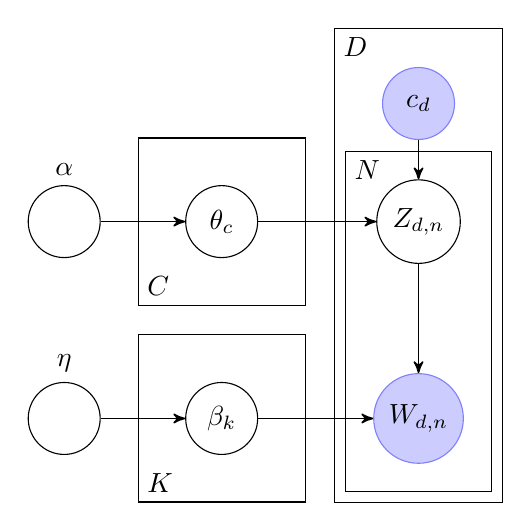
\begin{tikzpicture}
	[
	observed/.style={minimum size=26pt,circle,draw=blue!50,fill=blue!20},
	unobserved/.style={minimum size=26pt,circle,draw},
	post/.style={->,>=stealth',semithick},
	]
	
	\node (w-j) [observed] at (0,0) {$W_{d,n}$};
	\node (z-j) [unobserved, above of= w-j, node distance=2.5cm] {$Z_{d,n}$};
	\node (category_obs) [observed, above of= z-j, node distance=1.5cm] {$c_d$};
	\node (category_dist) [unobserved, left of=z-j, node distance=2.5cm] {$\theta_c$};
	\node (alpha-hyper) [unobserved, label=above:$\alpha$, left of=category_dist, node distance=2cm] {};
	\node (beta-hyper) [unobserved, left of = w-j, node distance=2.5cm] {$\beta_k$};
	\node (eta-hyper) [unobserved, label=above:$\eta$, left of=beta-hyper, node distance=2cm] {};
	
	\path
	(z-j) edge [post] (w-j)
	(alpha-hyper) edge [post] (category_dist)
	(category_obs) edge [post] (z-j)
	(category_dist) edge [post] (z-j)
	(beta-hyper) edge [post] (w-j)
	(eta-hyper) edge [post] (beta-hyper)
	;
	
	\node [draw,fit=(w-j) (category_obs), inner sep=14pt] (plate-context) {};
	\node [below right] at (plate-context.north west) {$D$};
	
	\node [draw,fit=(w-j) (z-j), inner sep=10pt] (plate-token) {};
	\node [below right] at (plate-token.north west) {$N$};
	
	\node [draw,fit=(beta-hyper) (beta-hyper), inner sep=17pt] (plate-context) {};
	\node [above right] at (plate-context.south west) {$K$};
	
	\node [draw,fit=(category_dist) (category_dist), inner sep=17pt] (plate-context) {};
	\node [above right] at (plate-context.south west) {$C$};
\end{tikzpicture}
		}
		\caption{Category-topic model.}
		\label{fig:category_lda}
	\end{subfigure}
	\hspace{2em}
	\begin{subfigure}{0.275\textwidth}
		\centering
		\resizebox{\textwidth}{!}{%
			\begin{tikzpicture}
	[
	observed/.style={minimum size=26pt,circle,draw=blue!50,fill=blue!20},
	unobserved/.style={minimum size=26pt,circle,draw},
	post/.style={->,>=stealth',semithick},
	]
	
	\node (w-j) [observed] at (0,0) {$W_{d,n}$};
	\node (z-j) [unobserved, above of= w-j, node distance=2.5cm] {$Z_{d,n}$};
	\node (author_obs) [observed, above of= z-j, node distance=1.5cm] {$a_d$};
	\node (author_dist) [unobserved, left of=z-j, node distance=2.5cm] {$\theta_a$};
	\node (alpha-hyper) [unobserved, label=above:$\alpha$, left of=category_dist, node distance=2cm] {};
	\node (beta-hyper) [unobserved, left of = w-j, node distance=2.5cm] {$\beta_k$};
	\node (eta-hyper) [unobserved, label=above:$\eta$, left of=beta-hyper, node distance=2cm] {};
	
	\path
	(z-j) edge [post] (w-j)
	(alpha-hyper) edge [post] (author_dist)
	(author_obs) edge [post] (z-j)
	(author_dist) edge [post] (z-j)
	(beta-hyper) edge [post] (w-j)
	(eta-hyper) edge [post] (beta-hyper)
	;
	
	\node [draw,fit=(w-j) (author_obs), inner sep=14pt] (plate-context) {};
	\node [below right] at (plate-context.north west) {$D$};
	
	\node [draw,fit=(w-j) (z-j), inner sep=10pt] (plate-token) {};
	\node [below right] at (plate-token.north west) {$N$};
	
	\node [draw,fit=(beta-hyper) (beta-hyper), inner sep=17pt] (plate-context) {};
	\node [above right] at (plate-context.south west) {$K$};
	
	\node [draw,fit=(author_dist) (author_dist), inner sep=17pt] (plate-context) {};
	\node [above right] at (plate-context.south west) {$A$};
\end{tikzpicture}
		}
		\caption{Author-topic model.}
		\label{fig:author_lda}
	\end{subfigure}	
	\caption{Plate notation for the metadata \gls{lda} models.}
	\label{fig:metadata_lda}
\end{figure*}

\subsection{\acrlong{pam}}\label{subsec:pachinko_prelim}
The \acrfull{pam}~\cite{li2006pachinko} is a topic model that generalizes \gls{lda}, making it possible to construct topic hierarchies based on any \gls{dag} structure.
The model focuses on finding topics of different abstraction levels, as well as modeling the connections between these topics.

Each node in the \gls{dag} structure represents a topic in the pachinko allocation model. 
However, unlike \gls{lda} where topics are distributions over words, in \gls{pam} topics are distributions over words and/or other topics further down the hierarchy of the \gls{dag} structure.

\citet{li2006pachinko} present a Four-Level \gls{pam}, which is a layered \gls{pam} meaning that the \gls{dag} structure is divided into layers, with every node in a layer being fully connected to every node in the next layer of the hierarchy.
It consists of $L$ layers of varying sizes $S_0, S_1, \dots, S_{L-1}$.
The first layer consists of only the root node, a topic which all documents are part of.
The bottom layer consists of leaf nodes, which represent the words in the vocabulary.
The rest are middle layers representing topics of different abstraction levels.

$T = {t_1, t_2, \dots, t_s}$ is the set of topics in the \gls{pam}. 
Each topic $t_i$ is associated with a Dirichlet distribution $g_i(\alpha_i)$ based on a vector $\alpha_i$ which has the same dimension as the number of children in $t_i$.
While it is possible to use different $\alpha$ values for each topic, as shown below, we found through experimentation that using the same $\alpha$ value for all layers still provided good results.

The generative process for each document $d$ in \gls{pam} consists of the following steps, as described by \citeauthor{li2006pachinko}~\cite{li2006pachinko}:
\begin{enumerate}
	\item Sample $\theta_{t_1}^{(d)}, \theta_{t_2}^{(d)}, \dots, \theta_{t_s}^{(d)}$ from $g_1(\alpha_1), g_2(\alpha_2), \dots, \newline g_s(\alpha_s)$, where $\theta_{t_i}^{(d)}$ is a multinomial distribution of topic $t_i$ over its children.
	\item For each word $w \in d$,
	\begin{itemize}
		\item Sample a topic path $\mathbf{z}_w$ of length $L_w:~< z_{w1}, z_{w2},\newline \dots, z_{wL_w} >$. $z_{w1}$ is always the root and $z_{w1}$ through $z_{wL_w}$ are topic nodes in $T$. $z_{wi}$ is a child of $z_{w(i-1)}$ and it is sampled according to the multinomial distribution $\theta_{z_{wL_w}}^{(d)}$.
		\item Sample word $w$ from $\theta_{z_{wL_w}}^{(d)}$.
	\end{itemize}
\end{enumerate}

The intuition behind this generative process is to create all possible topic sequences and combine these into a multinomial distribution to draw a topic sequence from.
Otherwise, the Gibbs sampling is the same as with the \gls{lda} model.

The plate notation from \citet{li2006pachinko} and our modification can be seen in \autoref{fig:pachinko_plates}.

\begin{figure*}[ht]
	\centering
	\begin{subfigure}{0.40\textwidth}
		\centering
		\resizebox{\textwidth}{!}{%
			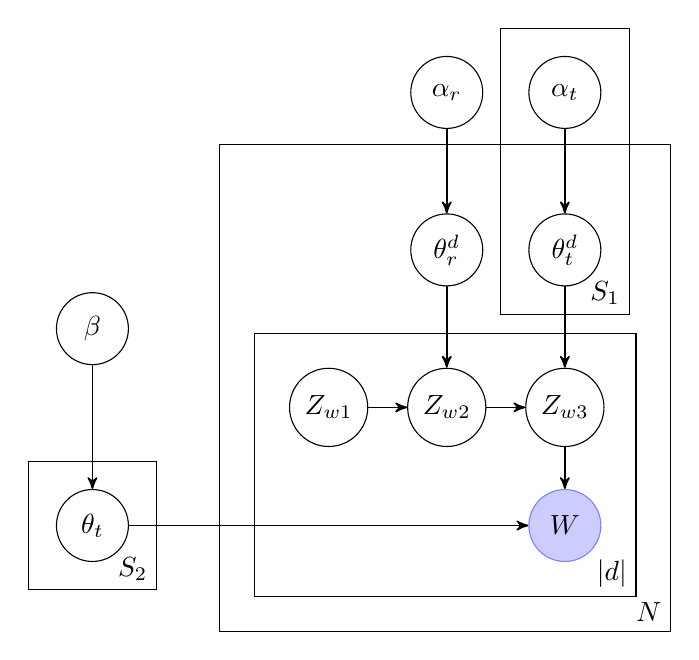
\begin{tikzpicture}
	[
	observed/.style={minimum size=26pt,circle,draw=blue!50,fill=blue!20},
	unobserved/.style={minimum size=26pt,circle,draw},
	post/.style={->,>=stealth',semithick},
	]
	
	\node (w-j) [observed] at (0,0) {$W$};
	\node (z-3) [unobserved, above of= w-j, node distance=1.5cm] {$Z_{w3}$};
	\node (z-2) [unobserved, left of= z-3, node distance=1.5cm] {$Z_{w2}$};
	\node (z-1) [unobserved, left of= z-2, node distance=1.5cm] {$Z_{w1}$};
	
	\node (theta_r) [unobserved, above of= z-2, node distance=2cm] {$\theta_r^d$};
	\node (alpha_r) [unobserved, above of= theta_r , node distance=2cm] {$\alpha_r$};
	
	\node (theta_k) [unobserved, above of= z-3, node distance=2cm] {$\theta_{t}^d$};
	\node (alpha_k) [unobserved, above of= theta_k , node distance=2cm] {$\alpha_{t}$};
	
	\node (theta_s2) [unobserved, left of=w-j , node distance=6cm] {$\theta_{t}$};
	\node (beta) [unobserved, above of=theta_s2 , node distance=2.5cm] {$\beta$};
	
	\path
	(z-3) edge [post] (w-j)
	(z-2) edge [post] (z-3)
	(z-1) edge [post] (z-2)
	
	(theta_r) edge [post] (z-2)
	(alpha_r) edge [post] (theta_r)
	
	(theta_k) edge [post] (z-3)
	(alpha_k) edge [post] (theta_k)
	
	(theta_s2) edge [post] (w-j)
	(beta) edge [post] (theta_s2)
	;
	
	\node [draw,fit=(w-j) (theta_r) (z-1), inner sep=25pt] (plate-context) {};
	\node [above left] at (plate-context.south east) {$N$};
	
	\node [draw,fit=(w-j) (z-1), inner sep=12.5pt] (plate-token) {};
	\node [above left] at (plate-token.south east) {$|d|$};
	
	\node [draw,fit=(theta_s2), inner sep=10pt] (plate-token) {};
	\node [above left] at (plate-token.south east) {$S_2$};
	
	\node [draw,fit=(theta_k) (alpha_k), inner sep=10pt] (plate-token) {};
	\node [above left] at (plate-token.south east) {$S_1$};
\end{tikzpicture}

		}
		\caption{Original Four-Level \gls{pam}.}
		\label{fig:four_layer_pachinko}
	\end{subfigure}
	\hspace{1em}
	\begin{subfigure}{0.40\textwidth}
		\centering
		\resizebox{\textwidth}{!}{%
			\begin{figure}[h]
	\centering
	\resizebox{0.8\columnwidth}{!}{%
	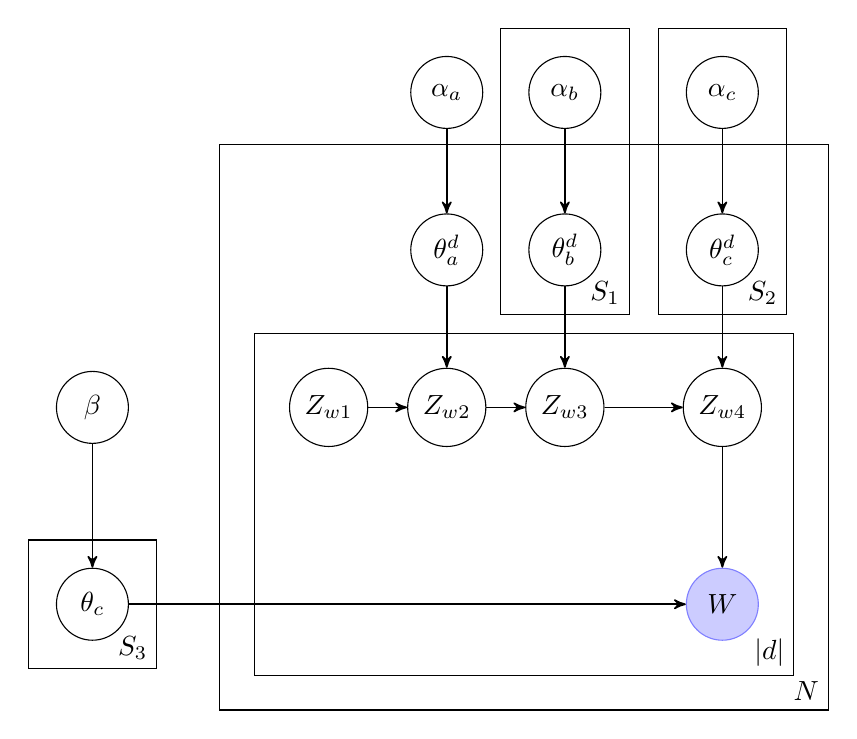
\begin{tikzpicture}
		[
		observed/.style={minimum size=26pt,circle,draw=blue!50,fill=blue!20},
		unobserved/.style={minimum size=26pt,circle,draw},
		post/.style={->,>=stealth',semithick},
		]
		
		\node (w-j) [observed] at (0,0) {$W$};
		\node (z-4) [unobserved, above of= w-j, node distance=2.5cm] {$Z_{w4}$};
		\node (z-3) [unobserved, left of= z-4, node distance=2cm] {$Z_{w3}$};
		\node (z-2) [unobserved, left of= z-3, node distance=1.5cm] {$Z_{w2}$};
		\node (z-1) [unobserved, left of= z-2, node distance=1.5cm] {$Z_{w1}$};
		
		\node (theta_a) [unobserved, above of= z-2, node distance=2cm] {$\theta_a^d$};
		\node (alpha_a) [unobserved, above of= theta_a , node distance=2cm] {$\alpha_a$};
		
		\node (theta_b) [unobserved, above of= z-3, node distance=2cm] {$\theta_b^d$};
		\node (alpha_b) [unobserved, above of= theta_b , node distance=2cm] {$\alpha_b$};
		
		\node (theta_c) [unobserved, above of= z-4, node distance=2cm] {$\theta_c^d$};
		\node (alpha_c) [unobserved, above of= theta_c , node distance=2cm] {$\alpha_c$};
		
		\node (theta_s2) [unobserved, left of=w-j , node distance=8cm] {$\theta_c$};
		\node (beta) [unobserved, above of=theta_s2 , node distance=2.5cm] {$\beta$};
		
		\path
		(z-4) edge [post] (w-j)
		(z-3) edge [post] (z-4)
		(z-2) edge [post] (z-3)
		(z-1) edge [post] (z-2)
		
		(theta_a) edge [post] (z-2)
		(alpha_a) edge [post] (theta_a)
		
		(theta_b) edge [post] (z-3)
		(alpha_b) edge [post] (theta_b)
		
		(theta_c) edge [post] (z-4)
		(alpha_c) edge [post] (theta_c)
		
		(theta_s2) edge [post] (w-j)
		(beta) edge [post] (theta_s2)
		;
		
		\node [draw,fit=(w-j) (theta_a) (z-1), inner sep=25pt] (plate-context) {};
		\node [above left] at (plate-context.south east) {$N$};
		
		\node [draw,fit=(w-j) (z-1), inner sep=12.5pt] (plate-token) {};
		\node [above left] at (plate-token.south east) {$|d|$};
		
		\node [draw,fit=(theta_s2), inner sep=10pt] (plate-token) {};
		\node [above left] at (plate-token.south east) {$S_3$};
		
		\node [draw,fit=(theta_c) (alpha_c), inner sep=10pt] (plate-token) {};
		\node [above left] at (plate-token.south east) {$S_2$};
		
		\node [draw,fit=(theta_b) (alpha_b), inner sep=10pt] (plate-token) {};
		\node [above left] at (plate-token.south east) {$S_1$};
		
	\end{tikzpicture}}
	\caption{Plate notation for the five-level \gls{pam}.}
	\label{fig:pachinko}
\end{figure}
\vejleder[inline]{a,b,c ~ $t_i$ in Figure 5}
		}
		\caption{Five-Level \gls{pam}.}
		\label{fig:five_layer_pachinko}
	\end{subfigure}
	\caption{Plate notation for the original Four-Level \gls{pam} and our Five-Level \gls{pam}.}
	\label{fig:pachinko_plates}
\end{figure*}

\section{Topic Models}\label{sec:plate_notation}
In this section, topic models that are explored in the experiment are detailed.
This covers the standard \gls{lda} from \citet{blei2003latent}, our category and author metadata models, which build on the concept of \gls{lda}, and our taxonomy metadata model, which uses the \acrlong{pam}.

\subsection{Standard \gls{lda}}
The purpose of \gls{lda}, and topic models in general, is to create a tool for exploring collections of text.
Topic models do this by uncovering the underlying semantic structure of a text collection by using hierarchical Bayesian models.
\Gls{lda} uncovers this semantic structure by discovering patterns of word use in documents and finding topics based on these~\cite{blei2009topic}.

The standard \gls{lda} by \citet{blei2003latent} can be described by the following generative process, which is the way the model assumes the documents arose:
$D$ is the number of documents in the corpus, $N_d$ is the number of words in document $d$, $V$ is the size of the vocabulary, and $K$ is the number of topics.
Topics are represented as distributions over words and documents are represented as distributions of topics.
\Gls{lda} assumes that the topics are shared across the corpus, while the document-topic distributions are unique for each document.
For each topic $k \in \{1,\dots, K\}$ a topic-word distribution $\beta_k$ is sampled from a V-dimensional Dirichlet distribution parameterized by $\eta$.
That is, K topics $\beta_{1:k}$ are sampled, each being a distribution over the vocabulary, written as: $\beta_k \sim Dirichlet(\eta)$.
Likewise, for each document $d \in \{1,\dots, D\}$ a document-topic distribution $\theta_d$ is sampled from a K-dimensional Dirichlet distribution parameterized by $\alpha$.
For each word $n \in \{1, \dots, N_d\}$ in each document $d$, a topic $z_{d,n}$ is sampled from a K-multinomial distribution $\theta_d$, and then a word $w_{d,n}$ is sampled from a V-multinomial distribution $\beta_{z_{d,n}}$.
The generative process for each document is seen in these steps:

\vspace{\topsep}
\begin{enumerate}
	\item Draw topic proportion $\theta_d \sim Dirichlet(\alpha)$
	\item For each word $n$ in the document:
	\begin{enumerate}
		\item Draw topic assignment $z_{d,n} \sim Mult(\theta_d)$
		\item Draw word $w_{d,n} \sim Mult(\beta_{z_{d,n}})$
	\end{enumerate}
\end{enumerate}
\vspace{\topsep}

The generative process for topics and documents, generates a list of $K$ topics and $D$ documents that can be used as a $K \times V$ matrix of topic-word distributions and a $D \times K$ matrix of document-topic distributions, respectively.
The plate notation for \gls{lda} can be seen in \autoref{fig:standard_lda}.

\begin{figure}[h]
  \centering
  \resizebox{\columnwidth}{!}{%
	  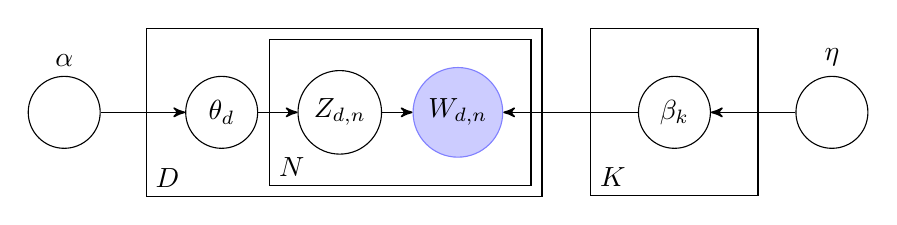
\begin{tikzpicture}
	    [
	      observed/.style={minimum size=15pt,circle,draw=blue!50,fill=blue!20},
	      unobserved/.style={minimum size=26pt,circle,draw},
	      post/.style={->,>=stealth',semithick},
	    ]
	
	    \node (w-j) [observed] at (0,0) {$W_{d,n}$};
	    \node (z-j) [unobserved] at (-1.5,0) {$Z_{d,n}$};
	    \node (theta) [unobserved] at (-3,0) {$\theta_d$};
	    \node (alpha-hyper) [unobserved, label=above:$\alpha$,left of=theta, node distance=2cm] {};
	    \node (beta-hyper) [unobserved] at (2.75,0) {$\beta_k$};
	    \node (eta-hyper) [unobserved, label=above:$\eta$, ,right of=beta-hyper, node distance=2cm] {};
	    
	    \path
	    (z-j) edge [post] (w-j)
	    (alpha-hyper) edge [post] (theta)
	    (theta) edge [post] (z-j)
	    (beta-hyper) edge [post] (w-j)
	    (eta-hyper) edge [post] (beta-hyper)
	    ;
	    
	    \node [draw,fit=(w-j) (theta), inner sep=14pt] (plate-context) {};
	    \node [above right] at (plate-context.south west) {$D$};
	    \node [draw,fit=(w-j) (z-j), inner sep=10pt] (plate-token) {};
	    \node [above right] at (plate-token.south west) {$N$};
	    \node [draw,fit=(beta-hyper) (beta-hyper), inner sep=17pt] (plate-context) {};
	    \node [above right] at (plate-context.south west) {$K$};
	  \end{tikzpicture}
  }
	\caption{Plate notation for \gls{lda}.}
	\label{fig:standard_lda}
\end{figure}

After training the \gls{lda} model, there are multiple possibilities for exploring the corpus using the posterior distributions of the hidden random variables.
One possibility is to visualize the posterior topics of the model, e.g., by sorting $\beta_k$ according to the highest probabilities.
It is also possible to visualize the documents by, e.g., sorting by the highest topic proportions in $\theta_d$.
Another possibility of exploration is finding similar documents by using a distribution distance function on the topic proportions $\theta_d$ between documents~\cite{blei2009topic}.

\subsection{Author-Topic \gls{lda} and Category-Topic \gls{lda}}
We model both of the metadata fields 'Author' and 'Category' similarly to the model presented by \citet{author_topic_2012}.
In this model, there are no document-topic distributions $\theta$.
Instead, each author and category has its own topic distribution.
This is based on the assumption that authors prefer to write about specific topics, and that categories of the articles were chosen based on the content of the finished article or that local newspapers have their own unique topic preferences.

Our topic models are \glspl{um}, meaning that topics are only word distributions and are chosen based on the data of the documents, rather than \glspl{dm} where topics are fitted to have an influence on both word distributions and other metadata.

\citet{author_topic_2012} describe the author-topic model where for each document $d$, they assign a vector of authors $a_d$ from a set of authors $A$, and for each word draw an author $x$ from this vector.
However, for our category-topic model and our own author-topic model, each document $d$ is associated with one category $c_d$ from a set of categories $C$ and one author $a_d$ from a set of authors $A$, rather than a vector.
This is due to our dataset never having more than one author or category for each document.
Unless otherwise stated, future mentions of the author-topic model are to our implementation of this model, rather than the model presented by \citet{author_topic_2012}.
The plate notation for our category and author \gls{lda} models can be seen in \autoref{fig:metadata_lda}.

\begin{figure*}[ht]
	\centering
	\begin{subfigure}{0.3\textwidth}
		\centering
		\resizebox{\textwidth}{!}{%
		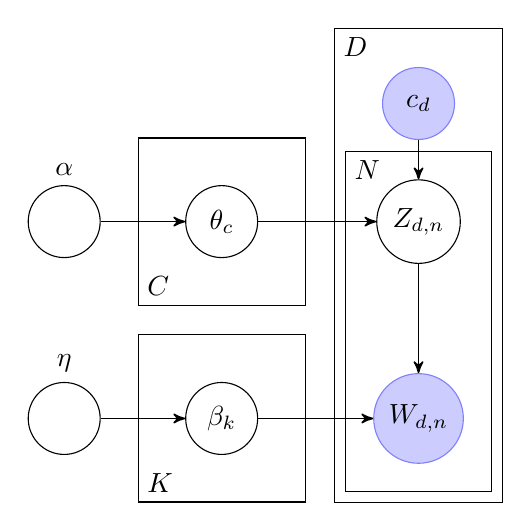
\begin{tikzpicture}
	[
	observed/.style={minimum size=26pt,circle,draw=blue!50,fill=blue!20},
	unobserved/.style={minimum size=26pt,circle,draw},
	post/.style={->,>=stealth',semithick},
	]
	
	\node (w-j) [observed] at (0,0) {$W_{d,n}$};
	\node (z-j) [unobserved, above of= w-j, node distance=2.5cm] {$Z_{d,n}$};
	\node (category_obs) [observed, above of= z-j, node distance=1.5cm] {$c_d$};
	\node (category_dist) [unobserved, left of=z-j, node distance=2.5cm] {$\theta_c$};
	\node (alpha-hyper) [unobserved, label=above:$\alpha$, left of=category_dist, node distance=2cm] {};
	\node (beta-hyper) [unobserved, left of = w-j, node distance=2.5cm] {$\beta_k$};
	\node (eta-hyper) [unobserved, label=above:$\eta$, left of=beta-hyper, node distance=2cm] {};
	
	\path
	(z-j) edge [post] (w-j)
	(alpha-hyper) edge [post] (category_dist)
	(category_obs) edge [post] (z-j)
	(category_dist) edge [post] (z-j)
	(beta-hyper) edge [post] (w-j)
	(eta-hyper) edge [post] (beta-hyper)
	;
	
	\node [draw,fit=(w-j) (category_obs), inner sep=14pt] (plate-context) {};
	\node [below right] at (plate-context.north west) {$D$};
	
	\node [draw,fit=(w-j) (z-j), inner sep=10pt] (plate-token) {};
	\node [below right] at (plate-token.north west) {$N$};
	
	\node [draw,fit=(beta-hyper) (beta-hyper), inner sep=17pt] (plate-context) {};
	\node [above right] at (plate-context.south west) {$K$};
	
	\node [draw,fit=(category_dist) (category_dist), inner sep=17pt] (plate-context) {};
	\node [above right] at (plate-context.south west) {$C$};
\end{tikzpicture}
		}
		\caption{Category \gls{lda}.}
		\label{fig:category_lda}
	\end{subfigure}
	\hspace{2em}
	\begin{subfigure}{0.3\textwidth}
		\centering
		\resizebox{\textwidth}{!}{%
			\begin{tikzpicture}
	[
	observed/.style={minimum size=26pt,circle,draw=blue!50,fill=blue!20},
	unobserved/.style={minimum size=26pt,circle,draw},
	post/.style={->,>=stealth',semithick},
	]
	
	\node (w-j) [observed] at (0,0) {$W_{d,n}$};
	\node (z-j) [unobserved, above of= w-j, node distance=2.5cm] {$Z_{d,n}$};
	\node (author_obs) [observed, above of= z-j, node distance=1.5cm] {$a_d$};
	\node (author_dist) [unobserved, left of=z-j, node distance=2.5cm] {$\theta_a$};
	\node (alpha-hyper) [unobserved, label=above:$\alpha$, left of=category_dist, node distance=2cm] {};
	\node (beta-hyper) [unobserved, left of = w-j, node distance=2.5cm] {$\beta_k$};
	\node (eta-hyper) [unobserved, label=above:$\eta$, left of=beta-hyper, node distance=2cm] {};
	
	\path
	(z-j) edge [post] (w-j)
	(alpha-hyper) edge [post] (author_dist)
	(author_obs) edge [post] (z-j)
	(author_dist) edge [post] (z-j)
	(beta-hyper) edge [post] (w-j)
	(eta-hyper) edge [post] (beta-hyper)
	;
	
	\node [draw,fit=(w-j) (author_obs), inner sep=14pt] (plate-context) {};
	\node [below right] at (plate-context.north west) {$D$};
	
	\node [draw,fit=(w-j) (z-j), inner sep=10pt] (plate-token) {};
	\node [below right] at (plate-token.north west) {$N$};
	
	\node [draw,fit=(beta-hyper) (beta-hyper), inner sep=17pt] (plate-context) {};
	\node [above right] at (plate-context.south west) {$K$};
	
	\node [draw,fit=(author_dist) (author_dist), inner sep=17pt] (plate-context) {};
	\node [above right] at (plate-context.south west) {$A$};
\end{tikzpicture}
		}
		\caption{Author \gls{lda}.}
		\label{fig:author_lda}
	\end{subfigure}
	\caption{Plate notation for the metadata \gls{lda} models.}
	\label{fig:metadata_lda}
\end{figure*}

\subsection{Pachinko Allocation}
In order to handle the hierarchical structure of the taxonomy metadata field, we use a hierarchical topic model, namely the \acrfull{pam} from \citet{li2006pachinko}.
Pachinko allocation generalizes \gls{lda}, making it possible to construct topic hierarchies based on any \gls{dag} structure.
\gls{pam} is a topic model focusing on finding topics of different abstraction levels and modeling the connections between these topics. 

Each node in the \gls{dag} structure represents a topic in the pachinko allocation model. 
However, unlike \gls{lda} where topics are distributions over words, in \gls{pam} topics are multinomial distributions over words and/or other topics further down the hierarchy of the \gls{dag} structure.
An example of the \gls{dag} structure used in this paper is shown in \autoref{fig:pachinko_dag}.

In this paper, we use a layered \gls{pam} meaning that the \gls{dag} structure is divided into layers, with every node in each layer fully connected to every node in the next layer of the hierarchy.
The first layer consists of only the root node, a topic which all documents are part of, and the bottom layer consists of leaf nodes, which are the only nodes to contain distributions over words, and they have no other topics in their distribution.

We replicate some layers in our \gls{dag} structure based on the structure from the taxonomy field within our dataset, having some nodes represent a topic based on a specific taxonomy.
To make the algorithm construct the topics to be based on our taxonomies, we introduce a novel locking mechanism for the Gibbs sampler which we use to run \gls{pam}.
This mechanism is discussed further in \autoref{subsec:mod_pachinko}.

We use a five-level pachinko tree structure, following the format presented by \citet{li2006pachinko}.
The first layer is the root layer.
The last layer is the word layer consisting of one node for each word in the vocabulary of our corpus.
The second and third layers will be constructed based on the entries of the first two positions in our taxonomy metadata, meaning there will be one node for each unique sub-taxonomy entry that is in the first or second position in the taxonomy sequence (e.g. "STEDER" and "Danmark", which is taken from "STEDER/Danmark/Aalborg", but not "Aalborg" since it is in the third position).
We only use the first two layers for this, as these are among the most informative, and because introducing even more layers would slow down the training exponentially, since the probability of all possible combinations of topics needs to be sampled for every word during training.
The fourth layer consists of $K = 90$ 'blank' topics, as with the other models we present in this paper.
This layer is added so that the model can construct its own topics based on the higher-level topics learned from our taxonomy metadata.
This \gls{dag} structure is visualized in \autoref{fig:pachinko_dag}.

The generative process for each document $d$ in \gls{pam} consists of the following steps, as described by \citet{li2006pachinko}:
\begin{enumerate}
	\item Sample $\theta_{t_1}^{(d)}, \theta_{t_2}^{(d)}, \dots, \theta_{t_s}^{(d)}$ from $g_1(\alpha_1), g_2(\alpha_2), \dots, \newline g_s(\alpha_s)$, where $\theta_{t_i}^{(d)}$ is a multinomial distribution of topic $t_i$ over its children.
	\item For each word $w \in d$,
	\begin{itemize}
		\item Sample a topic path $\mathbf{z}_w$ of length $L_w: < z_{w1}, z_{w2}, \dots, z_{wL_w} >$. $z_{w1}$ is always the root and $z_{w1}$ through $z_{wL_w}$ are topic nodes in $T$. $z_{wi}$ is a child of $z_{w(i-1)}$ and it is sampled according to the multinomial distribution $\theta_{z_{wL_w}}^{(d)}$.
		\item Sample word $w$ from $\theta_{z_{wL_w}}^{(d)}$.
	\end{itemize}
\end{enumerate}

$T = {t_1, t_2, \dots, t_s}$ os the set of topics in the \gls{pam}. 
Each topic $t_i$ is associated with a Dirichlet distribution $g_i(\alpha_i)$ based on a vector $\alpha_i$ which has the same dimention as the number of children in $t_i$.
While it is possible to use different $\alpha$ values for each topic, as shown here, we found through experimentation that using the same $\alpha$ value for all layers still provided good results.
An illustration of the plate notation for \gls{pam} can be found in \autoref{fig:pachinko}.

We use Gibbs sampling for performing inference.
For each word, a chain of topics is sampled by calculating the probability of all combinations of topics and making a weighted sample.
The probability of each topic combination is calculated using the joint probability of the topics, as presented in \autoref{eq:pachinko_gibbs}.

\begin{equation}\label{eq:pachinko_gibbs}
	\begin{split}
		P(Z_{w2} = t_a, Z_{w3} = t_b, Z_{w4} = t_c | \textbf{D}, z_{-w}, \alpha, \beta) \propto \\
		\frac{n_{1a}^d + \alpha_{1a}}{n_1^d + \sum_{a'} \alpha_{1a'}} \times
		\frac{n_{ab}^d + \alpha_{ab}}{n_a^d + \sum_{b'} \alpha_{ab'}}  \times 
		\frac{n_{bc}^d + \alpha_{bc}}{n_{b}^d + \sum_{c'} \alpha_{bc'}} \\ \times 
		\frac{n_{cw}^d + \beta_{w}}{n_{c} + \sum_{m} \beta_{m}} 
	\end{split}
\end{equation}
As in \citet{li2006pachinko}, $Z_{w2}$, $Z_{w3}$, $Z_{w4}$ are topic assignments for the three middle layers of topics in our 5-layer Pachinko model.
The root topic is not part of this equation since all words are part of it, so the probability does not need to be calculated.
$Z_{-w}$ is the word topic assignment, for all other words except the one that is being updated.
$n_x^d$ is the number of times topic $t_x$ occurs in document $d$ according to $Z_{-w}$. 
The $n_{xy}^d$ describes how many times topic $t_y$ is sampled from its parent $t_x$ within document $d$ according to $Z_{-w}$.
$n_x$ is the number of times topic $t_x$ occurs in the corpus according to $Z_{-w}$, and $n_{xw}$ is the number of times a word $w$ is in $t_x$ according to $Z_{-w}$.

\begin{figure}
	\centering
	\resizebox{0.8\columnwidth}{!}{%
	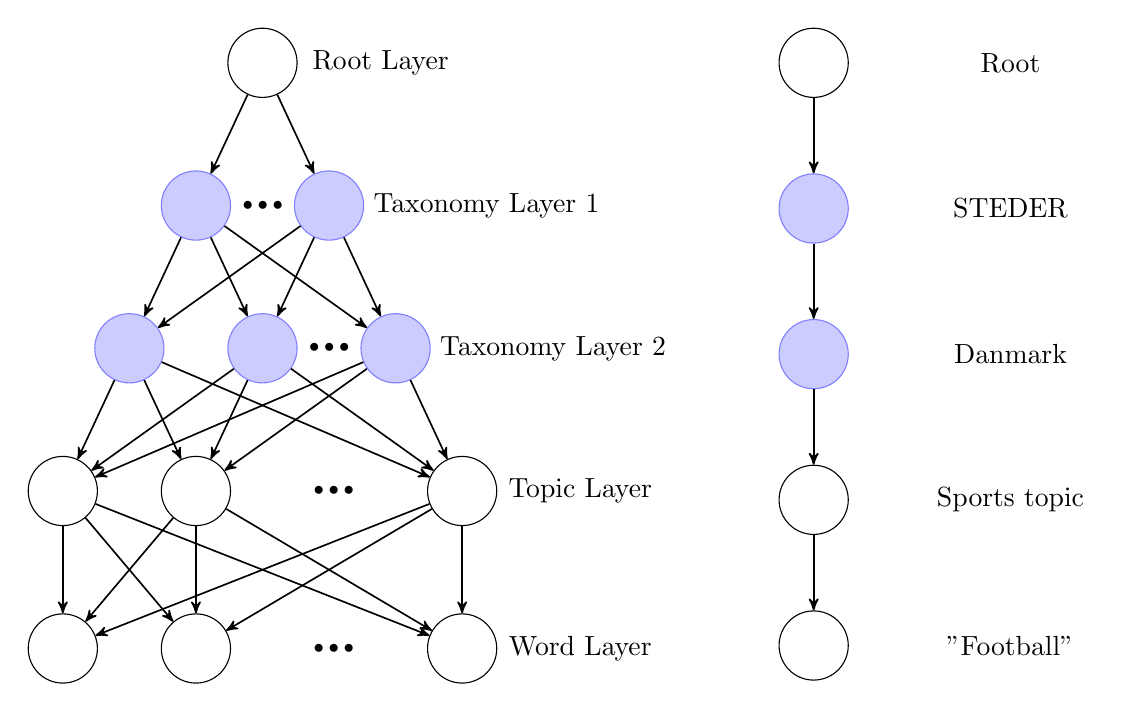
\begin{tikzpicture}
		[
		observed/.style={minimum size=25pt,circle,draw=blue!50,fill=blue!20},
		unobserved/.style={minimum size=25pt,circle,draw},
		post/.style={->,>=stealth',semithick},
		]
		% Layer 0
		\node (top) [unobserved] at (0,0) {};
		\node (topname) [right of = top, node distance=1.5cm] {Root Layer};
		
		% Layer 1
		\node (l11) [observed] at ([shift=({245:2 cm})]top) {};
		\node (l12) [observed] at ([shift=({295:2 cm})]top) {};
		\node (l1_dots) [right of = l11, node distance=0.85cm] {\scalebox{0.75}{$\bullet\bullet\bullet$}};
		\node (1name) [right of = l12, node distance=2cm] {Taxonomy Layer 1};
		
		% Layer 2
		\node (l21) [observed] at ([shift=({245:2 cm})]l11) {};
		\node (l22) [observed] at ([shift=({295:2 cm})]l11) {};
		\node (l23) [observed] at ([shift=({295:2 cm})]l12) {};
		\node (l2_dots) [right of = l22, node distance=0.85cm] {\scalebox{0.75}{$\bullet\bullet\bullet$}};
		\node (2name) [right of = l23, node distance=2cm] {Taxonomy Layer 2};
		
		% Layer 3
		\node (l31) [unobserved] at ([shift=({245:2 cm})]l21) {};
		\node (l32) [unobserved] at ([shift=({295:2 cm})]l21) {};
		\node (l33) [unobserved] at ([shift=({295:2 cm})]l23) {};
		\node (l2_dots) [right of = l32, node distance=1.75cm] {\scalebox{0.75}{$\bullet\bullet\bullet$}};
		\node (3name) [right of = l33, node distance=1.5cm] {Topic Layer};
		
		% Layer 4
		\node (l41) [unobserved] at ([shift=({270:2 cm})]l31) {};
		\node (l42) [unobserved] at ([shift=({270:2 cm})]l32) {};
		\node (l43) [unobserved] at ([shift=({270:2 cm})]l33) {};
		\node (l2_dots) [right of = l42, node distance=1.75cm] {\scalebox{0.75}{$\bullet\bullet\bullet$}};
		\node (4name) [right of = l43, node distance=1.5cm] {Word Layer};
		
		\path
		% Layer 0
		(top) edge [post] (l11)
		(top) edge [post] (l12)
		
		% Layer 1
		(l11) edge [post] (l21)
		(l11) edge [post] (l22)
		(l11) edge [post] (l23)
		(l12) edge [post] (l21)
		(l12) edge [post] (l22)
		(l12) edge [post] (l23)
		
		% Layer 2
		(l21) edge [post] (l31)
		(l21) edge [post] (l32)
		(l21) edge [post] (l33)
		(l22) edge [post] (l31)
		(l22) edge [post] (l32)
		(l22) edge [post] (l33)
		(l23) edge [post] (l31)
		(l23) edge [post] (l32)
		(l23) edge [post] (l33)
		
		% Layer 3
		(l31) edge [post] (l41)
		(l31) edge [post] (l42)
		(l31) edge [post] (l43)
		(l32) edge [post] (l41)
		(l32) edge [post] (l42)
		(l32) edge [post] (l43)
		(l33) edge [post] (l41)
		(l33) edge [post] (l42)
		(l33) edge [post] (l43)
		;
		
		
		\node (root) [unobserved, node distance=1.85cm] at (7,0) {};
		\node (rootname) [right of = root, node distance=2.5cm] {Root};
		
		\node (first) [observed, below of=root, node distance=1.85cm] {};
		\node (firstname) [right of = first, node distance=2.5cm] {STEDER};
		
		\node (second) [observed, below of=first, node distance=1.85cm] {};
		\node (secondname) [right of = second, node distance=2.5cm] {Danmark};
		
		\node (third) [unobserved, below of=second, node distance=1.85cm] {};
		\node (thirdname) [right of = third, node distance=2.5cm] {Sports topic};
		
		\node (fourth) [unobserved, below of=third, node distance=1.85cm] {};
		\node (fourthname) [right of = fourth, node distance=2.5cm] {"Football"};
		
		
		\path
		% Layer 0
		(root) edge [post] (first)
		(first) edge [post] (second)
		(second) edge [post] (third)
		(third) edge [post] (fourth)
		;
		
\end{tikzpicture}}
\end{figure}


\begin{figure}[h]
	\centering
	\resizebox{0.8\columnwidth}{!}{%
	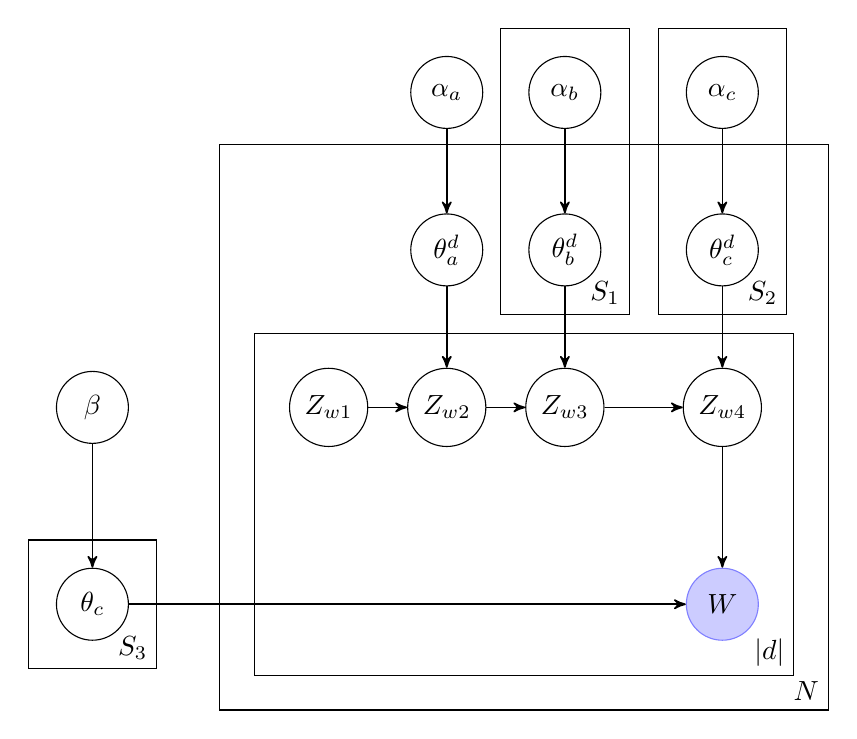
\begin{tikzpicture}
		[
		observed/.style={minimum size=26pt,circle,draw=blue!50,fill=blue!20},
		unobserved/.style={minimum size=26pt,circle,draw},
		post/.style={->,>=stealth',semithick},
		]
		
		\node (w-j) [observed] at (0,0) {$W$};
		\node (z-4) [unobserved, above of= w-j, node distance=2.5cm] {$Z_{w4}$};
		\node (z-3) [unobserved, left of= z-4, node distance=2cm] {$Z_{w3}$};
		\node (z-2) [unobserved, left of= z-3, node distance=1.5cm] {$Z_{w2}$};
		\node (z-1) [unobserved, left of= z-2, node distance=1.5cm] {$Z_{w1}$};
		
		\node (theta_a) [unobserved, above of= z-2, node distance=2cm] {$\theta_a^d$};
		\node (alpha_a) [unobserved, above of= theta_a , node distance=2cm] {$\alpha_a$};
		
		\node (theta_b) [unobserved, above of= z-3, node distance=2cm] {$\theta_b^d$};
		\node (alpha_b) [unobserved, above of= theta_b , node distance=2cm] {$\alpha_b$};
		
		\node (theta_c) [unobserved, above of= z-4, node distance=2cm] {$\theta_c^d$};
		\node (alpha_c) [unobserved, above of= theta_c , node distance=2cm] {$\alpha_c$};
		
		\node (theta_s2) [unobserved, left of=w-j , node distance=8cm] {$\theta_c$};
		\node (beta) [unobserved, above of=theta_s2 , node distance=2.5cm] {$\beta$};
		
		\path
		(z-4) edge [post] (w-j)
		(z-3) edge [post] (z-4)
		(z-2) edge [post] (z-3)
		(z-1) edge [post] (z-2)
		
		(theta_a) edge [post] (z-2)
		(alpha_a) edge [post] (theta_a)
		
		(theta_b) edge [post] (z-3)
		(alpha_b) edge [post] (theta_b)
		
		(theta_c) edge [post] (z-4)
		(alpha_c) edge [post] (theta_c)
		
		(theta_s2) edge [post] (w-j)
		(beta) edge [post] (theta_s2)
		;
		
		\node [draw,fit=(w-j) (theta_a) (z-1), inner sep=25pt] (plate-context) {};
		\node [above left] at (plate-context.south east) {$N$};
		
		\node [draw,fit=(w-j) (z-1), inner sep=12.5pt] (plate-token) {};
		\node [above left] at (plate-token.south east) {$|d|$};
		
		\node [draw,fit=(theta_s2), inner sep=10pt] (plate-token) {};
		\node [above left] at (plate-token.south east) {$S_3$};
		
		\node [draw,fit=(theta_c) (alpha_c), inner sep=10pt] (plate-token) {};
		\node [above left] at (plate-token.south east) {$S_2$};
		
		\node [draw,fit=(theta_b) (alpha_b), inner sep=10pt] (plate-token) {};
		\node [above left] at (plate-token.south east) {$S_1$};
		
	\end{tikzpicture}}
	\caption{Plate notation for the five-level \gls{pam}.}
	\label{fig:pachinko}
\end{figure}
\vejleder[inline]{a,b,c ~ $t_i$ in Figure 5}

\subsubsection{Modification to Pachinko Allocation}\label{subsec:mod_pachinko}
Without modification, \gls{pam} will find topics with the same structure as our taxonomy, but the topics will not actually be based on the taxonomy.
However, only $25\%$ of the documents in our dataset have an observed taxonomy.
To account for this, we lock taxonomy for the words in the observed documents to be in the corresponding topics within the pachinko \gls{dag} instead of continuously sampling them using Gibbs sampling.
This creates a constant context for the taxonomy topics, which the documents with unobserved taxonomies will be fitted around.

Some of the observed documents have multiple taxonomies.
For these documents, one of the taxonomies is chosen randomly for each word in the document.


%
%\input{sections/method/preprocessing}
%\input{sections/method/method.tex}
%\input{sections/method/query_handling.tex}

%\section{Dataset}
Nordjyske is a Danish news agency that maintains multiple newspapers, radios and other news sources throughout north Jutland, a region in Denmark.
They store their news articles in a non-public database, where each article contains multiple meta-data fields which describes some aspect of the data eg. author.
The dataset is from 2017 to 2019 and contains 139261 articles which uses a vocabulary of 69192 unique words.
One of the metadata fields is the Category field, which both describes where the article is supposed to be located(within a newspaper) and also which subject the article is about.
These meta-data are very interesting in that they detail the data in certain ways which might be useful in some way.

In the following section, we describe each of the meta-data fields which are analysed.

\subsection{Author}
This field mentions the author, who have written the article.
Each article only has a single author, so we do not account for multiple authors in this paper.
This field is fully observed within the dataset, which means that every article has an author.
There are $227$ different authors within the dataset and they are almost evenly distributed in the number of articles they have written.

\subsection{Category}
The category field describes a variety of different aspects. 
This field is fully observed within the dataset and there are $58$ different categories.
A proportion of the articles contains which specific newspaper, they belong to, eg. Aalborg-Newspaper.
Another proportion of the category fields describes the overall theme, such as Culture and Sports-newspaper.

\subsection{Taxonomy}
The taxonomy field describes a hierarchical structure of the topical or geographical subject of the articles.
This field is only partially observed within the dataset, which means that roughly $50\%$ of the articles contain this field.
We observe a general pattern when traversing this field which is:
\begin{itemize}
	\item Places/Country/Region/Town
	\item Topics/Sub-Topic/Subsub-topic
\end{itemize}
Examples of this field are:
\begin{itemize}
	\item PLACES/Danmark/Nordjylland/Aalborg/Lillevorde
	\item TOPICS/Religion/Christianity
\end{itemize}
%%\input{sections/Pipeline.tex}
\section{Evaluation}\label{sec:experiment}
In this section, we evaluate the topic models previously defined.
We also define the evaluation metrics and how hyperparameters for the models were chosen.
Lastly, the results of the evaluations are displayed.

\subsection{Models}\label{sec:experiment_models}
A list of different topic models is evaluated each using different metadata from the dataset.
The main difference between the models is how they draw a specific topic for a word.
As detailed in \autoref{sec:plate_notation} the main models used in this experiment are:
\begin{description}
	\item[\Acrlong{lda}] Standard \gls{lda} which uses document-topic distributions.
	\item[Author-Topic Model]\cite{author_topic_2012} An \gls{lda} based model, which uses author-topic distributions.
	\item[Category-Topic Model] An \gls{lda} based model which uses category-topic distributions.
	\item[Taxonomy-Topic Model] A \acrlong{pam} which uses hierarchical taxonomy information.
\end{description}

\subsection{Evaluation Metrics}\label{sec:experiment_metrics}
\vejleder[inline]{fix commas in this section}
All models previously mentioned are evaluated using the following evaluation metrics.

The main metric used in this experiment is the topic coherence metric.
This metric indicates how semantically similar the top words within each topic are and is an indication of the topic quality within a model~\cite{topic_coherence_2015}.
There are different methods for calculating topic coherence, but we will be using $C_v$ coherence.
$C_v$ is calculated using the following steps, as presented by~\citet{Syed2017coherence}:
\begin{enumerate}
	\item Topic-word segmentation into word set pairs
	\item Word and word pair probability calculation
	\item Word set confirmation measure
	\item Aggregation of confirmation measures
\end{enumerate}
The intuition is to calculate the degree of semantic similarity between highly probable words in a topic.
This intuition, and each step, is explained further in Appendix \autoref{app:topic_coherence}.

The second metric used in the experiment is perplexity.
Perplexity is used as a metric to show how well a model can predict new test samples $w_d$.
But because perplexity is not specific to topic models and by itself does not give an indication of how coherent topics are, it is used as a secondary evaluation~\cite{tea_leaves}.
To calculate perplexity, we first need to compute the log-likelihood of $w_d$, which is done in:
\begin{equation}\label{eq:likelihood}
	\mathcal{L}(w_d) = \log p(w_d|\Phi) = \sum_{d} \log p(w_d|\Phi)
\end{equation}
\noindent where $\Phi$ is the topic-word matrix.
The perplexity measure is then calculated as follows:
\begin{equation}
	\emph{Perplexity}(w_d) = exp \{-\frac{\mathcal{L}(w_d)}{W}\}
\end{equation}
\noindent where W is the number of words \cite{de2008evaluating}.

The second metric used in the experiment is topic difference.
Topic difference is another metric that is used to check the quality of the topic model.
It is based on the assumption that a good topic model will have little overlap between topics.
It is therefore not the best measure of the final quality of a topic model but a low topic difference will indicate potential problems with a model.
\begin{equation}
	\emph{TopicDifference} = \frac{1}{K \cdot K} \sum_{i=1}^{K} \sum_{j=1}^{K} JS(\beta_{i},\beta_{j})
\end{equation}
\noindent where $JS$ is Jensen-Shannon distance, $K$ is the number of topics, and $\beta_{k}$ is the topic-word distribution for topic $k$.
If the total sum is not averaged, it can also be used to indicate the convergence of the model.

\subsection{Grid Search}\label{sec:experiment_gridsearch}
To find the optimal hyperparameter values for the models, we run a grid search.
To find the best performing model we test different values of $K$, $\alpha$, and $\eta$ in a grid search.
Specifically, we run two rounds of grid search.
In the first round, the number of topics $K$ we test are the values of $K_1$, as seen in \autoref{tab:gridsearch}, with randomly chosen $\alpha$ and $\eta$ values for each $K$ value.
This creates much fewer runs of the grid search to start with and eliminates hyperparameter values that give worse models.
In the second round, the number of topics $K$ we test are the values of $K_2$ with all combinations of $\alpha$ and $\eta$ except for those with values of $0.001$, since these models gave much worse scores.
The hyperparameter values used are shown in \autoref{tab:gridsearch}.

We only run the grid search on the standard \gls{lda} model, with the assumption that the number of topics that perform well for this model also performs well for the metadata models when the same dataset is used.
To evaluate the \gls{lda} models, we measure the topic coherence of a model after training it on the dataset for 50 epochs, and the hyperparameters of the model with the highest score are then used for the models in the rest of the experiment.

Based on the topic coherence of the model, we choose $K = 90$, $\alpha = 0.01$, and $\eta = 0.1$ as the hyperparameters for all models in the experiment.

\begin{table}[t]
	\centering
	\caption{Tested hyperparameter values for the grid search. $K_2$ are the $K$ values used for the grid search in conjunction with the bolded values in $\alpha$ and $\eta$.}
	\begin{tabular}{c|c}
		Parameter & Tested Values\\
		\midrule
		$K_1$ & 10, 20, 30, $\dots$, 100, 150\\
		$K_2$ & 50, 60 70, 80, 90, 100\\
		$\alpha$ & \textbf{0.1}, \textbf{0.01}, 0.001\\
		$\eta$ & \textbf{0.1}, \textbf{0.01}, 0.001\\
	\end{tabular}
	\label{tab:gridsearch}
\end{table}


\subsection{Results}\label{sec:results}

\begin{table}[h]
	\centering
	\caption{Results.}
	\begin{tabular}{l|c|c}
		Topic Model & \makecell{Topic \\ Coherence} & \makecell{Topic \\ Difference} \\
		\midrule
		\Acrlong{lda} & 0.520 & 0.575 \\
		Author-Topic Model & 0.335 & 0.615 \\
		Category-Topic Model & 0.370 & 0.560 \\
		Taxonomy-Topic Model & \textbf{0.660} & \textbf{0.709} \\
	\end{tabular}
	\label{tab:metric_results}
\end{table}

From \autoref{tab:metric_results}, we can see that the Author and Category-Topic models are performing the worst, whereas the Taxonomy-Topic model is outperforming all other models.
However, the elapsed time of the taxonomy-topic model is worse than the standard \gls{lda}.
It takes about $6$-$8$ hours to compute $50$ epochs for the \gls{lda} model, depending on the CPU. 
The taxonomy-topic model running a $5$ layered \gls{pam} took ${\sim}132$ hours before completing the $50$ epochs.
Analysis of the topics in the trained models is given in \autoref{sec:discussion}.
Extended analysis and other models are investigated in Appendix \autoref{subsec:app_exten_models} and \autoref{app:cat_auth_pachinko}.


%% - Body(50 \%)
%%	- Results 
%
%%	- Discussion
%%		- Main results
%%		- Other results
%%		- Error sources
\section{Discussion}\label{sec:discussion}
In this section, we investigate the different models to see how each meta-information field impacts the resulting topics.
Firstly, we want to investigate the top words within each model.
We have taken a random article from the dataset and visualized how the topics differ between the models. 
Before investigating the article below, we define a specific color scheme for each model.

In the article, we have highlighted the highest probable words within the three most occurring topics in the article.
The article is about agriculture and how farmers are letting their cows out onto grass fields in September. 
It also mentions a few different farms in the Northern part of Jutland and describes these in various ways.

The way we can compare these models, is by taking the top 200 words for each topic-word distribution within each model and marking them in the article below.
Since the Author and Category models do not have a document-topic distribution we can not look at the specific document, but instead we have marked the words from the given category- and author-topic distribution within the document, to see what the difference in topics are.
We are looking at the top 3 topics within each model for the specific document.

\begin{table}[h]
	\centering
	\caption{Color scheme for each model.}
	\begin{tabular}{l|c}
		Topic Model & Color \\
		\midrule
		\Acrlong{lda} & \thiscolor{Goldenrod} \vspace*{2mm} \\
		Author-Topic Model & \thiscolor{Aquamarine} \vspace*{2mm} \\
		Category-Topic Model & \thiscolor{LimeGreen} \vspace*{2mm} \\
		Word appearing in multiple models & \thiscolor{Peach} \vspace*{2mm}  \\
	\end{tabular}
	\label{tab:disc_color}
\end{table}

\emph{
Kig på grise, køer og kyllinger10 \colorbox{Peach}{nordjyske} bedrifter åbner \colorbox{LimeGreen}{søndag} for stalddørene Landbruget åbner \colorbox{LimeGreen}{søndag} 16. \colorbox{Peach}{september} ladeporte og stalddøre for offentligheden. 52 danske bedrifter er med i årets ”Åbent landbrug”. I det \colorbox{Peach}{nordjyske} kan man kigge forbi på 10 \colorbox{Peach}{forskellige} landbrug. Blandt de \colorbox{Peach}{nordjyske} deltagere er der \colorbox{Peach}{mulighed} for at få indsigt i både kvæg- og svinebedrifter, \colorbox{Peach}{ligesom} en producent af slagtekyllinger \colorbox{Aquamarine}{byder} velkommen. Sidstnævnte kan opleves hos Rokkedahl i Farstrup. De er tre familier med i alt \colorbox{Peach}{seks} børn, der sammen driver Rokkedahl Landbrug med slagtekyllinger og planteproduktion \colorbox{Peach}{samt} Rokkedahl Energi, som laver energioptimering. Herudover har de \colorbox{Goldenrod}{eget} slagteri, hvor ca. 35 af deres i alt 65 \colorbox{Peach}{medarbejdere} arbejder. Familien Rokkedahl har \colorbox{Peach}{arbejdet} med kyllinger siden 1963 og er tredje generation. I staldene og i de omkringliggende folde har de både fritgående og økologiske slagtekyllinger. Velfærdskyllingerne går i flokke og har adgang til store folde. På årsbasis opdrætter Rokkedahl \colorbox{Peach}{otte} \colorbox{Peach}{millioner} kyllinger som enten slagtes på deres \colorbox{Goldenrod}{eget} slagteri eller sælges til eksterne slagterier. På de 1350 \colorbox{Goldenrod}{hektar} har de hvede, byg raps, havre, rug, ærter og hestebønner. Det anvendes primært til foder til velfærdskyllingerne. De dyrker \colorbox{Peach}{jorden} primært økologisk og anvender halmen til opvarmning af staldene. De har varmevekslere på alle stalde for at minimere varmeforbruget og ammoniakudledningen til omgivelserne. Britt og Klaus Kristiansen på Solbakken Agri ved Aabybro er \colorbox{Peach}{klar} til vise en stor, \colorbox{Peach}{dansk} mælkeproduktion frem. Familien tæller også de fire børn, Maria på 18 år, Daniel på 16 år, Kamilla og Laura på 13 år, og de er sjette generation på gården, som de overtog i 2013. Solbakken har 600 økologiske malkekøer, som tilsammen \colorbox{Peach}{giver} 17.000 liter mælk om dagen. Den bliver hentet og kørt til et af Arlas mejerier, hvor den bliver anvendt til økologiske mejeriprodukter. 575 \colorbox{Goldenrod}{hektar} \colorbox{Peach}{land} tilhører gården, og her producerer \colorbox{Goldenrod}{familien} foder til deres \colorbox{Peach}{dyr} \colorbox{Peach}{samt} andre fødevarer.  I Himmerland kan man besøge Sanne og Ole Mathiasen, der driver Nørregaard på Braulstrupvej 9 i Suldrup. Her kan man se søer, smågrise og slagtesvin i staldene og \colorbox{Aquamarine}{høre} om \colorbox{Goldenrod}{produktion} af velfærdsgrise, se maskinerne, få smagsprøver fra Danish Crown og på \colorbox{Peach}{lokale} fødevarer, og \colorbox{Aquamarine}{høre} om biavl. For \colorbox{Aquamarine}{børnene} er der \colorbox{LimeGreen}{leg} i korncontainer og halm, pedaltraktorbane og ponytrækketure. Der er kaffe og kagebord. Åbent \colorbox{Goldenrod}{landbrug} foregår \colorbox{LimeGreen}{søndag} fra \colorbox{LimeGreen}{klokken} 10 til 16. Det er gratis at deltage. Sidste år deltog 96.000 \colorbox{LimeGreen}{danskere} i åbent landbrug.
}

Overall, we see that there is a large amount of overlap between the models, which is interesting since the models use different meta-information to create the various topic distributions.
This indicates that the models share many of the top words, while also indicating a slight deviation between the models due to the meta-information.
The \gls{lda} model shows words like "landbrug" (agriculture) and "produktion" (production), which is what the article is mostly about.
This behavior is to be expected since the performance of \gls{lda} has been explored and evaluated before. 
Author-topic specific words are not very present and are only showing three unique words: "byder", "hører", and "børnene".
This indicates that the Author-topic model has trouble generalizing what the author of this article (Peter Tordrup Larsen) is writing about, possibly because he has written $5002$ articles in our dataset.
Another aspect of the Author-Topic model is that the authors writing these articles most likely do not write about just one subject, which explains why there is only three less important words marked here. 
The Category-topic model only shows four unique words: "søndag", "leg", "klokken", and "danskere".
These words are also very abstract and can be used in many different scenarios.

An interesting part of this analysis is the words appearing in multiple models.
Some of the words within this category are: "arbejdet", "jorden", "dyr", and "nordjyske".
These words summarize the text pretty well, but it is also hard to summarize this text since it covers a wide variety of specific topics.
Combining the results of these models might yield better topic models, but we can not conclude that based on only one article.
There is also the possibility that choosing another random article would give completely different numbers of marked words per model, because this highly depends on the article's author and category.


\subsection{Author-topic model}\label{sec:discussion_author_topic}
Some interesting observations can also be made specifically in the author-topic model.
One observation that is possible, is looking at the similarity of authors.
In this model, the author-topic distribution defines the probabilities of topics being written by a specific author.
Then, just as \citet{author_topic_2012}, the similarity of authors can be found by calculating the symmetric Kullback-Leibler divergence:

\begin{equation}
	sKL(i,j) = \sum_{t=1}^{T}\left[\theta_{it}\, log \frac{\theta_{it}}{\theta_{jt}} + \theta_{jt}\, log \frac{\theta_{jt}}{\theta_{it}}\right]
\end{equation}
\noindent where $\theta_{it}$ is the probability of author $i$ having written about topic $t$, and the same for $\theta_{jt}$ with author $j$.

In the context of using these similarities to assist Nordjyske, knowing how similar authors are gives the opportunity to recommend new authors to readers, while the articles are about similar topics.
In \autoref{tab:author_similarity} the top 10 author pairs, based on this similarity measure, are shown.
A smaller KL value means the authors are more similar.
The number in parenthesis next to each author is the number of articles they have written in our dataset.

\begin{table}[h]
	\centering
	\caption{Top 10 author pairs based on the symmetric KL divergence between authors.}
	\begin{tabular}{r|c}
		Author pair & KL \\
		\midrule
		Lars Termansen (328) \& Mikkel Færgemann Viken (91) & 1.50 \\
		Morten Nis Klenø (17) \& Anne Helene Thomsen (606) & 1.72 \\
		Lars Termansen (328) \& Lars Christensen (1293) & 2.43 \\
		Esben Heine Pedersen (1689) \& Caspar Birk (71) & 2.47 \\
		Lars Christensen (1293) \& Poul Christoffersen (65) & 2.53 \\
		Lone Beck (92) \& Max Melgaard (587) & 2.74 \\
		HANNE Lindblad Jensen (27) \& Peter Tordrup Larsen (5002) & 2.94 \\
		Søren Kjær (95) \& Carl Chr. Madsen (785) & 2.98 \\
		Heidi Majgaard B. Pedersen (244) \& Lisbeth Helleskov (361) & 3.05 \\
		Lars Termansen (328) \& Morten Lind (413) & 3.16 \\
		\midrule
		Maximum & 34.51 \\
		Median & 24.20 \\
	\end{tabular}
	\label{tab:author_similarity}
\end{table}

In general for these pairs, there does not seem to be a correlation between a high similarity and the categories of the articles they have written.
While one author in a pair might have written for the sports category (Sport-avis) the other author might not have written for this category at all.
This can also be seen for categories that cover geographic locations, where one author might have written for Aalborg (Aalborg-avis) and the other author can have written for Thisted (Thisted-avis).

When looking at a sample of documents for the most similar author pair (Lars Termansen \& Mikkel Færgemann Viken), it is seen that they both write a mix of regular news and sports articles.
The reason why they become this similar, might be that the ratio between news and sports news for both authors is similar, and possibly also because of the types of news they write about.
Another interesting observation is that, for the second most similar author pair (Morten Nis Klenø \& Anne Helene Thomsen) the difference in the number of articles written is significant.
Here Morten Nis Klenø has written just 17 articles while Anne Helene Thomsen has written 606 articles.
This suggests that some part of why these authors' similarity is high, simply dependents on the types of news the authors have written, no matter the amount.

It is also worth noting that while authors that write scientific papers usually write in just a few subject areas, the scientific area they work in, this is not the case for news article authors.
In our dataset, this can be seen in the fact that the authors have written for 7.86 categories on average, with 7 categories as the median.
This can make it more difficult for the author-topic model to find patterns in what the authors write about, especially since each category can cover multiple topics.

A selection of authors from the dataset and the top words from their most probable topics, can be seen in \autoref{tab:author_top_words}.

\begin{table*}[h]
	\centering
	\caption{Selection of authors and the top 10 words from their most probable topic.}
	\begin{tabular}{c|c|c|c|c|c|c}
		\toprule
		Birgitte Bové & Kirsten Østergaard & Pauline Bülow & Karen Marie Foldbjerg & Claus T. Kræmmergård & Hanne Lindblad Jensen & Ole Jensen \\
		\midrule
		Topic 41 & Topic 50 & Topic 3 & Topic 13 & Topic 88 & Topic 2 & Topic 50 \\
		\midrule
		\makecell{millioner \\ eu \\ hans \\ større \\ bedre \\ formand \\ kr \\ nordjyske \\ taget \\ skriver} & \makecell{du \\ thisted \\ unge \\ mig \\ børn \\ procent \\ hans \\ hver \\ penge \\ hjørring} & \makecell{procent \\ bag \\ rigtig \\ lave \\ dansk \\ formand \\ gode \\ klar \\ svært \\ plads} & \makecell{du \\ sine \\ formand \\ seneste \\ jensen \\ hvert \\ nyt \\ hvordan \\ finde \\ kommunen} & \makecell{du \\ procent \\ unge \\ børn \\ arige \\ hans \\ dansk \\ mig \\ thisted \\ mener} & \makecell{du \\ thisted \\ procent \\ mig \\ børn \\ hans \\ unge \\ dansk \\ mener \\ a} & \makecell{du \\ thisted \\ unge \\ mig \\ børn \\ procent \\ hans \\ hver \\ penge \\ hjørring} \\
		\bottomrule
	\end{tabular}
	\label{tab:author_top_words}
\end{table*}

As can be seen through this analysis, this knowledge about authors and their topic probabilities can be useful for making better news recommendation systems, but it will be limited since news authors usually write about multiple subjects.

%
%
%% - Conclusion (5 \%)
%%	- (Possible) Future work
\section{Conclusion}\label{sec:conclusion}
In this paper, we explore possibilities for incorporating metadata into existing topic models, such as \gls{lda} and \gls{pam}.
We evaluate these models based on three different metadata: Author, Category, and Taxonomy, each of which represents the data in a different way.

From the topic coherence results, shown in \autoref{tab:metric_results}, the \gls{pam} model using the Taxonomy metadata gets the best results.
The Author and Category models based on \gls{lda} are the worst-performing, where the topic coherence is much lower than the other models.

We want to answer the problem statement, which we stated in \autoref{sec:introduction}:


\begin{itemize}
	\item \textit{How does including metadata within the \gls{lda} model impact the resulting topics?}
	\item \textit{What possible problems can these models help alleviate at Nordjyske?}
	\begin{itemize}
		\item \textit{More specifically, how can these models improve recommendation?}
	\end{itemize}
\end{itemize}

We incorporate metadata into our topic models in multiple ways.
The \gls{lda} model is used as a baseline, which indicates whether incorporating metadata can improve the topic quality of our topic models.
Based on the results of Author-Topic and Category-Topic, we see that only using the metadata for topic assignment within \gls{lda} can hurt the topic quality.
Other studies have shown that only using the metadata for topic assignment can improve the performance.
This might be due to the particularities of the dataset, such as authors not usually writing about the same subject within the news environment.  


We use the \gls{pam} to incorporate a hierarchically structured metadata called Taxonomy, where we use a novel locking mechanism to lock the observed metadata's topics into place.
Using this model and technique, we can get better topic quality and words within \gls{pam} compared to the \gls{lda}.
However, the run time of the algorithm is quite slow compared to the \gls{lda}.
All models ran for 50 epochs, but \gls{pam} had a runtime of 130 hours, compared to \gls{lda} which had a runtime of 8 hours.

Topic modeling can be used to alleviate many problems at Nordjyske, such as recommendations.
We can use the topic distributions from our models to compare articles based on their similarity in topics.
For example, the author-topic model's topic distribution can be used to recommend similar authors, while in the topic distributions of the taxonomy model, there is the possibility of looking at topics from different layers.
This information can be used in a content-based filtering approach to recommend similar articles.
We suggest using this topic information to enrich the recommendation process at Nordjyske. 

Due to the promising results provided by the modified pachinko model, investigating this model further might be beneficial to incorporating metadata into topic models.
However, testing these models on multiple datasets needs to be accounted for since the generalizability of these models is not explored within this paper.
Using word embedding to further improve the performance of models can also be viewed as a possible next step for this project since a wide number of papers are using this technique to improve topic modeling\cite{MetaLDA2017}\cite{dieng2020topic}.

It would also be interesting to see how we could incorporate these models into an existing IT infrastructure at Nordjyske.
The next step in that process would be to investigate which part of their infrastructure could benefit from the use of topic modeling, whether it is for recommendation or automatic tagging of articles. 
We have written about a few potential use cases of our project in Section \ref{sec:appendix_applications} in the Appendix. 

%
%\input{sections/Acknowledgements}

% - References (10 \%)
% 	- Acknowledgments
%	- Bibliography
\bibliography{paper}

%Appendixes, if needed, appear before the acknowledgment.
\glsresetall
\onecolumn
\appendix
% Intro and overview
In the main paper, we initialize and describe our problem with a focus on results and analysis.
Within this appendix, we are expanding on many aspects of the aforementioned paper and new extensions to the models.
Following is an overview over each section and what it investigates.

\begin{enumerate}
	\item Metadata labels
	\begin{itemize}
		\item The metadata is shown in tables for all three metadata types, and observations about the metadata labels are described.
	\end{itemize} 
	\item Topic coherence
	\begin{itemize}
		\item We explain the purpose and mathematical ideas behind the evaluation metrics we use in the paper.
	\end{itemize} 
	\item Grid search 
	\begin{itemize}
		\item Our grid search process is described further on how we chose our hyperparameters.
	\end{itemize}
	\item Coloring articles 
	\begin{itemize}
		\item Two more articles are highlighted the same way as in \autoref{sec:discussion} and are analyzed.
	\end{itemize}
	\item Stemming the dataset 
	\begin{itemize}
		\item An experiment using a stemmed dataset is described, and the results are shown.
	\end{itemize}
	\item Pyro model implementation
	\begin{itemize}
		\item We describe the probabilistic programming language Pyro which we explored before choosing to work with Gibbs sampling.
	\end{itemize}
	\item Gibbs sampling
	\begin{itemize}
		\item The code for the Gibbs sampler is explained and investigated. A parallel Gibbs sampling method is also mentioned.
	\end{itemize}
	\item Pachinko implementation
	\begin{itemize}
		\item The implementation of our \gls{pam} model and how it differs from the Gibbs sampling method is explained.
	\end{itemize}
	\item Category and author \gls{pam}
	\begin{itemize}
		\item We go into detail about how we are using author and category metadata in the \gls{pam} and what results were achieved.
	\end{itemize}
	\item The author-category model
	\begin{itemize}
		\item We also combine the author-topic and category-topic models into one model with two topic distributions. This model is also analyzed.
	\end{itemize}
	\item The author-doc and category-doc models
	\begin{itemize}
		\item We create two new models called the author-doc and category-doc model. These models are a combination of the standard \gls{lda} and the author and category metadata.
	\end{itemize}
	\item Applications of our models
	\begin{itemize}
		\item We explore the application possibilities of our project and propose various applications which could be implemented at news sites such as Nordjyske.
	\end{itemize}
\end{enumerate}

\subsection{Overview}\label{sec:overview}
This section describes the steps of our method on an abstract level.
\autoref{fig:process_figure} visualizes these steps as a flowchart.
The method takes a corpus as an input and produces evaluation results as output.
Each step of the method is described in later sections in more detail.

\subsubsection*{Step 1: Preprocessing Phase}
In this step, we apply different preprocessing methods to simplify the dataset and remove redundant information.
Details of this phase are given in \autoref{sec:dataset}.
After finishing this phase, we are left with $139,060$ articles and $69,192$ unique words to form the corpus, which will be used in the following steps.

\subsubsection*{Step 2: \Gls{lda} Models}
In this step, we train the standard \gls{lda} model, the category, author, and taxonomy metadata models, as well as a combination model called the author-category model, on the corpus.
The standard \gls{lda} model and the metadata models are described further in \autoref{sec:plate_notation}, and the combination model is described in \autoref{sec:combination}.
The models are trained based on topic coherence, and after the training process the models are evaluated further.

\subsubsection*{Step 3: Evaluation of \gls{lda} Models}
In this step, we setup an experiment to evaluate the topic models trained in the previous step.
The evaluation metrics chosen for the experiment are perplexity and topic coherence.
Along with these evaluation metrics, human evaluation of the topics generated is also done to get a deeper understanding of what the models learn.
The experiment and results are presented in \autoref{sec:experiment} and are analyzed and discussed in \autoref{sec:discussion}.

\todo[inline]{Change/add more to the section as we figure out specifically what we do.}

\tikzstyle{process} = [rectangle, rounded corners, minimum width=2cm, minimum height=1cm,text centered, draw=black, fill=gray!50]
\tikzstyle{decision} = [diamond, minimum width=2cm, minimum height=1cm, text centered, draw=black, fill=green!30]

% one line
%\begin{figure}[ht]
%    \centering
%    \begin{tikzpicture}[node distance=2cm]
%    %\draw[step=1cm,gray,very thin] (-8,-8) grid (8,8);
%	\node (Dataset) [process] {(Input) Nordjyske Dataset};
%	\node (Cleaning)[process, below of=Dataset] {(1) Preprocessing Phase};
%	\node (Training) [process, below of=Cleaning] {(2)Train IR Methods};
%	\node (Query) [process, below of=Training] {(3) Query Generation};
%	\node (Evaluate) [process, below of=Query] {(4) Evaluate Models};
%	\node (Result) [process, below of=Evaluate] {(Output) Results};
%	\draw [->, very thick] (Dataset) edge (Cleaning); 
%	\draw [->, very thick] (Cleaning) edge (Training);
%	\draw [->, very thick] (Training) edge (Query);
%	\draw [->, very thick] (Query) edge (Evaluate);
%	\draw [->, very thick] (Evaluate) edge (Result);
%\end{tikzpicture}
%	\caption{The method visualized as a flowchart, where a dataset consisting of articles is processed into a list of ranked results.}
%    \label{fig:process_figure}
%\end{figure}

\begin{figure}[ht]
	\centering
	\begin{tikzpicture}[node distance=6em]
	%\draw[step=1cm,gray,very thin] (-8,-8) grid (8,8);
	\node (Dataset) [process, label=left:{Input}] {Nordjyske Dataset};
	\node (Cleaning)[process, below of=Dataset, label=left:{Step 1}] {Preprocessing};
	\node (Training) [process, below of=Cleaning, label=left:{Step 2}] {Train Topic Models};
	%\node (Query) [process, below of=Dataset, label=Step 3, yshift=2.5cm] {Query Generation};
	\node (Evaluate) [process, below of=Training, label=left:{Step 3}] {Evaluate Topic Models};
	\node (Result) [process, below of=Evaluate, label=left:{Output}] {Results};
	\draw [->, very thick] (Dataset) edge (Cleaning); 
	\draw [->, very thick] (Cleaning) edge (Training);
	\draw[->, very thick] (Training) edge (Evaluate);
	%\draw [->, very thick] (Query) edge (Evaluate);
	\draw [->, very thick] (Evaluate) edge (Result);
	\end{tikzpicture}
	\caption{The method visualized as a flowchart, where a dataset consisting of articles is processed into a list of evaluation results.}
	\label{fig:process_figure}
\end{figure}


% Expansions to sections from paper
\subsection{Metadata labels}\label{sec:appendix_meta_data}
In this section, the different types of metadata used in our evaluations will be explored. 
Here the focus will be on observations related to the labels of the metadata.

\subsubsection{Metadata labels}\label{sec:appendix_meta_data}
Here are the 58 different categories, which make up all the category labels present within the dataset.

\begin{table*}[h]
	\centering
	\begin{tabular}{l|c|l|c|l|c|l|c}
		Category & Number & Category & Number & Category & Number & Category & Number \\
 		\toprule
		Udland-avis & 8855 & 26. Frederik & 484 & INFOMAKER PRINT & 5 & Thisted sport & 698\\
		Kram & 244 & Feature & 188 & Thisted-net & 3 & WEEKEND & 1493\\
		Navne & 3749 & Morsø-avis & 5959 & DF Licitation Diverse & 4 & Erhverv-avis & 7356\\
		Brønderslev-net & 3857 & Aalborg-avis & 5544 & Oplandsavisen & 6 & Biler & 13\\
		Fælles & 20204 & Mariagerfjord-avis & 7241 & Morsø Sport & 2350 & Sport-net & 3\\
		Bo Godt & 1447 & Erhvervsnavne & 39 & Debat & 10075 & Frieord & 1341\\
		RB & 3 & Hanbo-bladet & 2 & Lokalavisen & 1 & Indsigt & 984\\
		Samfund & 9 & Morsø Debat & 1375 & Sport-avis & 10941 & Kultur & 3012 \\
		53. Frederik & 203 & DF Søfart & 32 & Bagside & 1933 & Morsø-net & 1 \\
		Frederikshavn-avis & 4325 & Nordjyske Biler & 1400 & Østvendsyssel Avis & 4 & Aalborg:nu & 73\\
		Perspektiv & 613 & Brønderslev-avis & 3857 & Rebild-avis & 4415 & Brugermappe & 1\\
		Thisted-avis & 11473 & DF Motor Biler & 3 & Nyhedsmotoren-net & 3 & Morsø Ugeavis & 27\\
		Jammerbugt-avis & 3791 & MitLiv & 1519 & Newspack & 35 & DF Licitation Byggeri & 14\\
		Mariagerfjord-net & 1 & Hjørring-avis & 4235 & Friii & 2333 & Vesthimmerland-avis & 5131\\
		Plus Publicering & 3 & Nordjyske Plus & 6 & & & & \\
		\bottomrule
	\end{tabular}
	\caption{Amount of documents with each category within the Nordjyske dataset from 2017 to 2019.}
	\label{tab:category_table}
\end{table*}

\subsubsection{Author Metadata}
There are a total of $227$ authors within the dataset where each author on average have written $757$ articles from 2017 to 2019.
An interesting fact is that the median is $316$ which is much lower than the average which is visible in \autoref{fig:author_histogram}.
This shows that while most authors have written just a few hundred articles, there is a small amount of authors that have written thousands of articles, increasing the average.
The minimum number of articles that have been written by an author is $1$ and the maximum number is $9906$.
When we look at the top two most writing authors, we get these:
\begin{itemize}
	\item Ove Nørhave (9893 articles)
	\begin{itemize}
		\item A well-known journalist, who have been at Nordjyske for over 25 years.
	\end{itemize}
	\item System Administrator (9038 articles)
	\begin{itemize}
		\item We are not sure why this has been used, it could be a placeholder.
	\end{itemize}
\end{itemize}

 
\begin{figure}
	\centering
	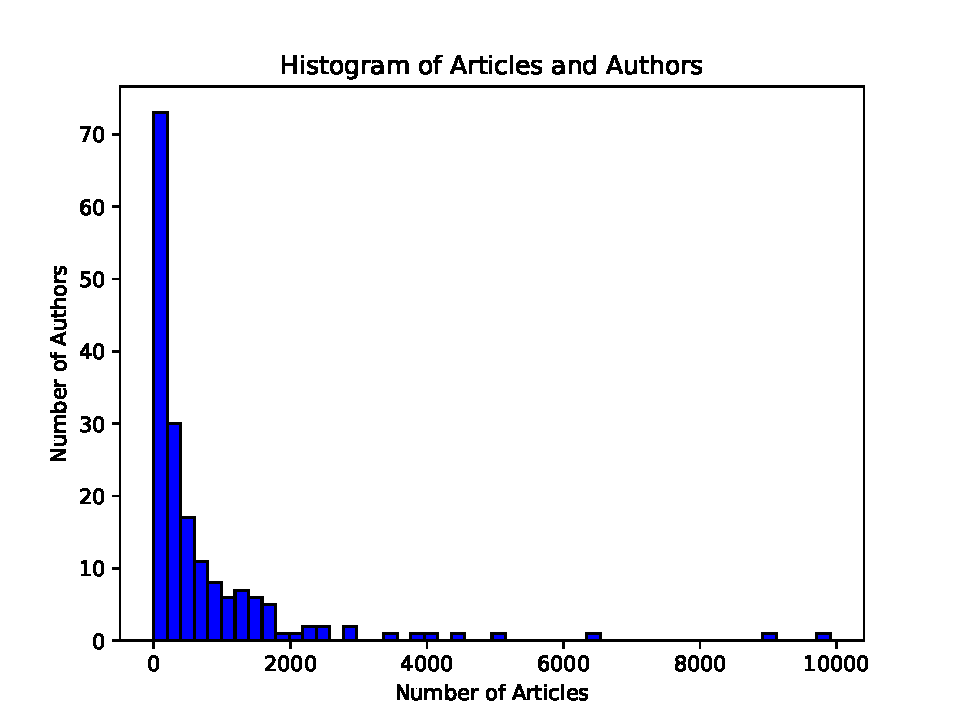
\includegraphics[width=.7\linewidth]{figures/author_hist_plot.pdf}
	\caption{A histogram over the number of articles authors have written.}
	\label{fig:author_histogram}
\end{figure}
In \autoref{fig:author_histogram}, we see that the vast majority of authors have written under $2000$ articles within the three years. 
All authors and the number of articles they have written can be seen in \autoref{tab:author_table}.

Other than the 'System Administrator' author, there are a few authors that seem different since they do not have the name of a person.
These are: 'SAXoTECH Systembruger' with 1 article, 'JSLbruger Nordjyske', 'testbruger', and 'Danske Fagmedier master' with 2 articles, and 'AAArtikler parkeret' with 51 articles.
After preprocessing, only 'AAArtikler parkeret' will not be put into the 'misc' author, since it has more than 13 articles.
From their names, they seem to be test users or authors that cover specific articles.
From looking at some articles these authors have written this seems to be the case since there are no obvious patterns in the articles written.
The name 'AAArtikler parkeret' also indicates that these articles, at least at some point, were unfinished and put under this author's name.

These articles are kept in our dataset, even though we can not be certain of who wrote them.

\begin{table*}[h]
	\caption{Number of documents written by each author in the Nordjyske dataset from 2017 to 2019.
	The highlighted authors are filtered and combined during preprocessing.}
	\label{tab:author_table}
	\centering
	\scriptsize
	\begin{tabular}{l|c|l|c|l|c|l|c}
		Author                & Number & Author                     & Number & Author                       & Number & Author                       & Number \\
		\midrule
		Ove Nørhave & 9893 & Bent Stenbakken & 646 & Katrine Schousboe & 189 & \textbf{Sarah Sandhøj} & 35 \\
		System Administrator & 9038 & Lars Hofmeister & 628 & Mathias Majlund Laursen & 178 & \textbf{Suzanne Tram} & 34 \\
		Ole Fink Mejlgaard & 6518 & Anne Helene Thomsen & 606 & Anne Brik Jensen & 177 & \textbf{Sebastian Engelberth Hansen} & 33 \\
		Peter Tordrup Larsen & 5002 & Max Melgaard & 587 & Peder Pedersen & 166 & \textbf{Anna Østergaard Bjørn} & 29 \\
		Kim Juhl Andersen & 4506 & Karen Marie Foldbjerg & 580 & Carl Åge Østergaard & 152 & \textbf{Michael Sand Andersen} & 27 \\
		Jeppe Damsgaard & 4057 & Lise Larsen & 575 & Mette Siggaard & 150 & \textbf{HANNE Lindblad Jensen} & 27 \\
		Jørn Larsen & 3863 & Asbjørn Hansen & 566 & Karen Keinicke & 150 & \textbf{Mathilde Juul Back Jensen} & 25 \\
		Jørn Eriksen & 3395 & Peter Witten & 544 & Tune Kristensen & 149 & \textbf{Allan Bauer} & 19 \\
		Anders Kjærgaard & 2960 & Allan Vinding Sørensen & 534 & Morten Brændstrup & 146 & \textbf{Linse Daugaard} & 18 \\
		Søren Beukel Bak & 2811 & Dorrit Gap Jensen & 530 & Emil Halkier & 143 & \textbf{Morten Nis Klenø} & 17 \\
		Søren Olsson & 2558 & Hans Christensen & 500 & \textbf{Britt Kristensen} & 135 & \textbf{OLE SANVIG KNUDSEN} & 16 \\
		Jens Peter Svarrer & 2480 & Lars Høj & 493 & \textbf{KAREN Marie Foldbjerg} & 132 & \textbf{Frederik Siiger} & 15 \\
		Flemming Kristensen & 2282 & Jesper Ramsing & 469 & \textbf{Claus Smidstrup} & 128 & \textbf{Kim Lesanner} & 15 \\
		Thomas Jasper & 2186 & Jens Hukiær & 464 & \textbf{Sarah Thun Madsen} & 127 & \textbf{Pia Haugaard} & 13 \\
		Bente Lembo & 2128 & Svend Ole Jensen & 447 & \textbf{Jakob Kanne Bjerregaard} & 126 & \textbf{MERETE HORN} & 12 \\
		Helle Møller Larsen & 1787 & Martin Frandsen & 437 & \textbf{Lars Teilmann} & 122 & \textbf{Regitze Ørnstrup Christensen} & 12 \\
		Claus Jensen & 1739 & Tobias Brandt & 423 & \textbf{Natasha Jahanshahi} & 117 & \textbf{Inge Steen Sørensen} & 11 \\
		Esben Heine Pedersen & 1689 & Andrea Jessen Jakobsen & 423 & \textbf{Jens Ole Pedersen} & 116 & \textbf{Anika Thorø Møller} & 11 \\
		Margit Sig & 1632 & Carsten Søgaard Jensen & 420 & \textbf{Pauline Bülow} & 116 & \textbf{Tim Søgaard} & 11 \\
		Jens Fogh-Andersen & 1614 & Morten Lind & 413 & \textbf{Christoffer Green Sørensen} & 115 & \textbf{Flemming Haslund} & 10 \\
		Ole Jensen & 1611 & Esben Agerlin Olsen & 406 & \textbf{Flemming Junker} & 103 & \textbf{Henrik Nordstrøm Mortensen} & 10 \\
		David Højmark & 1549 & Carsten Hougaard & 406 & \textbf{Niklas Grønborg} & 103 & \textbf{Emil Halkær} & 9 \\
		Niels Hansen & 1512 & Dorit Glintborg & 405 & \textbf{Sofie Møller} & 99 & \textbf{Katrine Hjulmann Nielsen} & 9 \\
		Line Lykkegaard Skou & 1504 & Karin Pedersen & 397 & \textbf{Michael Strandfelt} & 98 & \textbf{John Jensen} & 8 \\
		Lars Bang Bertelsen & 1443 & Kasper Ørkild & 393 & \textbf{Anders Sønderup} & 95 & \textbf{Jacob Eggert Kabel} & 8 \\
		Villy Dall & 1408 & Marianne Isen & 387 & \textbf{Søren Kjær} & 95 & \textbf{Søren Dietrichsen} & 7 \\
		Hans Peter Kragh & 1403 & Jakob Gammelgaard & 385 & \textbf{Lone Beck} & 92 & \textbf{Nicolai Østergaard} & 6 \\
		Claus T. Kræmmergård & 1354 & Dorte Geertsen & 383 & \textbf{Torben O. Andersen} & 91 & \textbf{Søren L. Hviid} & 6 \\
		Lars Christensen & 1293 & Torben Duch Holm & 364 & \textbf{Mikkel Færgemann Viken} & 91 & \textbf{Kathrine Lykkegaard Jeppesen} & 5 \\
		Rasmus Skovbo & 1253 & Henrik Strømgaard & 362 & \textbf{Hans Henrik Rasmussen} & 90 & \textbf{Ursula Rechnagel Taylor} & 5 \\
		Anders Abildgaard & 1229 & Lisbeth Helleskov & 361 & \textbf{Steffen Bek} & 89 & \textbf{Jens Otto Barsøe} & 4 \\
		Lasse Damsgaard & 1209 & Niels Brauer & 358 & \textbf{Simon Kjær Jensen} & 86 & \textbf{Maria Berg Badstue Pedersen} & 4 \\
		Søren Østergaard & 1207 & Jesper Poulsen & 348 & \textbf{Michael Sand} & 85 & \textbf{Jacob Andersen} & 3 \\
		Hanne Lindblad Jensen & 1191 & Lars Termansen & 328 & \textbf{Julian Drud Sørensen} & 84 & \textbf{Christian Brahe-Pedersen} & 3 \\
		Charlotte Bøje & 1117 & Mikkel Eklund & 328 & \textbf{Tina Larsen} & 82 & \textbf{Helle-Lise Ritzau Kaptain} & 3 \\
		Morten Kyndby Holm & 1102 & Susie Skov & 323 & \textbf{Nils Rasmussen} & 79 & \textbf{Jane Schmidt Klausen} & 3 \\
		Lars Aare Jensen & 1084 & Birgitte Sonne & 321 & \textbf{Katrine Hjulmann} & 73 & \textbf{Ebbe Fischer} & 3 \\
		Hanne Overbye & 1075 & Anders Andersen & 315 & \textbf{Mathias Lykke} & 72 & \textbf{Stefan Buur Hansen} & 3 \\
		Lise Stenbro & 1029 & Gunnar Onghamar & 309 & \textbf{Caspar Birk} & 71 & \textbf{Camilla Pehrson} & 2 \\
		Lone Lærke Krog & 1005 & Carl Emil Nielsen & 305 & \textbf{Anna Bech Sørensen} & 69 & \textbf{Danske Fagmedier master} & 2 \\
		Carsten Tolbøll & 1004 & Emma Toftelund Poulsen & 299 & \textbf{Fie Dømler} & 65 & \textbf{testbruger} & 2 \\
		Mette Møller & 974 & Ole Sanvig Knudsen & 287 & \textbf{Poul Christoffersen} & 65 & \textbf{Anders Fuglsang} & 2 \\
		Ida Smith & 973 & Charlotte Rørth & 276 & \textbf{Søren Skov} & 56 & \textbf{Peter Kargaard} & 2 \\
		Merete Horn & 929 & Morten Appel & 273 & \textbf{Nana Sofia Hansen} & 54 & \textbf{Morten Munk Andersen} & 2 \\
		Pernille K. Damsgaard & 922 & Kristian Gull Pedersen & 266 & \textbf{Tobias Reffstrup Rasmussen} & 53 & \textbf{JSLbruger Nordjyske} & 2 \\
		Lars Løcke & 873 & Birgitte Bové & 262 & \textbf{AAArtikler parkeret} & 51 & \textbf{Jan M. Jensen} & 1 \\
		Thomas Nielsen & 841 & Helle Madsen & 258 & \textbf{Camilla Gammelgaard Johansen} & 50 & \textbf{Tom Andersson} & 1 \\
		Jakob Frey Ahrentzen & 832 & Kasper Orkild Hansen & 255 & \textbf{Klaus Færch Gjerulff} & 49 & \textbf{Jørgen la Cour-Harbo} & 1 \\
		Lise Myrup Lassen & 793 & Emil Abkjær Kristensen & 253 & \textbf{Ida Thorsen} & 48 & \textbf{Rene Sonne} & 1 \\
		Carl Chr. Madsen & 785 & Nanna Holm Hansen & 252 & \textbf{Mathias Overgaard} & 46 & \textbf{SAXoTECH Systembruger} & 1 \\
		Inge Nørregård & 746 & Bine Martine Gori & 247 & \textbf{Kirsten Østergaard} & 45 & \textbf{Andreas K. Wielandt} & 1 \\
		Jesper Schouenborg & 724 & Heidi Majgaard B. Pedersen & 244 & \textbf{Gerda Buhl Andersen} & 44 & \textbf{Per Lyngby} & 1 \\
		Jens Sønderup & 709 & Daniel Vendner & 211 & \textbf{Pia Christensen} & 44 & \textbf{Michael F. Nørfelt} & 1 \\
		Birgit Eriksen & 700 & Ida Marie Kristensen & 204 & \textbf{Dorte Rohde} & 42 & \textbf{Simon Dinsen Hansen} & 1 \\
		Søren Wormslev & 681 & Kirsten Pilgaard & 197 & \textbf{Anna Grethe Jensen} & 41 & \textbf{Mads Skov Aagurd} & 1 \\
		Knud Labohn & 653 & Marianne Dyhrberg Cornett & 192 & \textbf{Henrik Schulz} & 38 & \textbf{Benita Dreyer-Andersen} & 1 \\
		Hans Jørgen Hansen & 646 & Susanne Justsen & 191 & \textbf{Lone Heilskov} & 37 & & \\
		\bottomrule
	\end{tabular}
\end{table*}

\subsubsection{Taxonomy}\label{subsec:appendix_taxonomy}
Taxonomy is fundamentally different from the other metadata fields, in this paper.
It is not fully observed with only roughly $25\%$ of documents having a taxonomy field.
It is hierarchical, with each taxonomy containing a sequence of sub-taxonomies, such as: 'STEDER/Danmark/Nordjylland/Aalborg'.
It is also possible for each document to have multiple taxonomy sequences.
Like with authors, we remove any sub-taxonomy that is used in less than $14$ taxonomy sequences ($0.01\%$ of the number of documents).
Out of $1135$ sub-taxonomies, $779$ are removed during this preprocessing.
A subset of the taxonomies and the number of articles they appear in can be seen in \autoref{tab:taxonomy_table}.
The taxonomy tree has the following sizes: 1, 4, 32, 90, and 69.192.
The numbers $4$ and $32$ are based on the number of unique taxonomy fields observed in the dataset.
The numbers $1$, $90$ and $69.192$ are the root, number of topics and number of words, respectively.

For the labels in \autoref{tab:taxonomy_table}, the counts show the labels' sizes.
It is worth mentioning that, while the counts of the labels are directly linked to the number of documents in the whole dataset, they are also connected to the size of the previous layer's taxonomy.
For example, the label 'Danmark' is in the layer below the 'STEDER' label, where the 26145 documents of 'Danmark' is a subset of the 29535 documents of 'STEDER'.

There is also a much larger number of 'STEDER' (places) documents compared to 'EMNER' (subjects) documents, respectively 29535 compared to 5449.
In \autoref{tab:taxonomy_table}, the first label on a lower layer that comes from 'EMNER' is 'Sport' with 408 documents.
This indicates that the subject taxonomies, in general, are much smaller in size.
The \gls{pam} will then be mostly influenced by this location information compared to actual topical labels.

The labels removed during preprocessing appear, as expected, to be places or subjects that have been written about just once or a few times.
We could have combined them into a 'misc' taxonomy as we did for the category and author metadata, but decided against it because it would just be a large collection of mostly random documents.

\begin{table*}[h]
	\caption{Number of documents written by each taxonomy in the Nordjyske dataset from 2017 to 2019.
	After sorting by the number of documents, only the first 100 and last 100 taxonomies are shown.
	The highlighted taxonomies are filtered and combined during preprocessing.}
	\label{tab:taxonomy_table}
	\centering
	\scriptsize
	\begin{tabular}{l|c|l|c|l|c|l|c}
		Taxonomy                & Number & Taxonomy                     & Number & Taxonomy                       & Number & Taxonomy                       & Number \\
		\midrule
		\emph{No taxonomy} & 103928 & Farsø & 182 & \textbf{Mallorca} & 1 & \textbf{Mali} & 1 \\
		STEDER & 29535 & Skørping & 177 & \textbf{Kloning} & 1 & \textbf{Godstransport} & 1 \\
		Danmark & 26145 & Hurup & 169 & \textbf{Hjørring revyen} & 1 & \textbf{Energiforbrug} & 1 \\
		Nordjylland & 23274 & Dronninglund & 167 & \textbf{Fredensborg} & 1 & \textbf{Gedser} & 1 \\
		EMNER & 5449 & Fjerritslev & 165 & \textbf{Iværksættere} & 1 & \textbf{Mylund} & 1 \\
		Thisted & 3592 & Aabybro & 163 & \textbf{Tall ships races} & 1 & \textbf{Bygge- og anlægsbranchen} & 1 \\
		Udland & 3390 & Frankrig & 159 & \textbf{Sproget} & 1 & \textbf{Kunstig intelligens} & 1 \\
		Aalborg & 3311 & Sverige & 158 & \textbf{Grurup} & 1 & \textbf{Nielstrup} & 1 \\
		Hjørring & 2146 & Paris & 157 & \textbf{Hørning} & 1 & \textbf{Kristiansand} & 1 \\
		Frederikshavn & 1997 & Fyn & 156 & \textbf{Hem} & 1 & \textbf{Nordborg} & 1 \\
		Mariagerfjord & 1987 & Rusland & 151 & \textbf{Floorball} & 1 & \textbf{Uggerhalne} & 1 \\
		Brønderslev & 1969 & Ulykker & 150 & \textbf{Store Brøndum} & 1 & \textbf{Barmer} & 1 \\
		Vesthimmerland & 1660 & Aarhus & 145 & \textbf{Korup} & 1 & \textbf{Narkomisbrug} & 1 \\
		Hovedstadsområdet & 1380 & Tyskland & 144 & \textbf{Fødevaresikkerhed} & 1 & \textbf{Adoption} & 1 \\
		Rebild & 1289 & Moskva & 143 & \textbf{Hammershøj} & 1 & \textbf{Fødevareindustri} & 1 \\
		Jammerbugt & 1198 & Arden & 142 & \textbf{Hjerneskade} & 1 & \textbf{Smugling} & 1 \\
		København & 1125 & Politik & 139 & \textbf{CATEGORY} & 1 & \textbf{Skikke og traditioner} & 1 \\
		Hobro & 996 & Morsø & 137 & \textbf{AaB Plus} & 1 & \textbf{Kigali} & 1 \\
		Aalborg og omegn & 833 & Berlin & 132 & \textbf{Ekstremsport} & 1 & \textbf{Holtet} & 1 \\
		Thisted og omegn & 800 & Sjælland & 131 & \textbf{Mozambique} & 1 & \textbf{Fritidshuse} & 1 \\
		Midtjylland & 783 & Løkken & 129 & \textbf{Maputo} & 1 & \textbf{Årslev} & 1 \\
		Mors & 630 & New York & 124 & \textbf{Handelsskole} & 1 & \textbf{Aalborg Håndbold} & 1 \\
		Aars & 540 & Natur & 123 & \textbf{Vendsyssel Håndbold} & 1 & \textbf{Oman} & 1 \\
		USA & 478 & Erhverv & 119 & \textbf{Biludstyr} & 1 & \textbf{Turistbranchen} & 1 \\
		Frederikshavn og omegn & 410 & Spanien & 119 & \textbf{Brandstiftelse} & 1 & \textbf{Øl} & 1 \\
		Sport & 408 & Klitmøller & 118 & \textbf{Nørre Dråby} & 1 & \textbf{Forlystelsespark} & 1 \\
		England & 381 & Aalestrup & 118 & \textbf{Stae} & 1 & \textbf{Etiopien} & 1 \\
		London & 379 & Herning & 116 & \textbf{Rebild Bakker} & 1 & \textbf{Addis Abeba} & 1 \\
		Hjørring og omegn & 369 & Stockholm & 115 & \textbf{Kampsport} & 1 & \textbf{Lystsejlads} & 1 \\
		Løgstør & 368 & Madrid & 115 & \textbf{Lynnedslag} & 1 & \textbf{Herfølge} & 1 \\
		Mariagerfjord og omegn & 364 & Jerslev & 113 & \textbf{Frederikshavn White Hawks} & 1 & \textbf{Sexchikane} & 1 \\
		Brønderslev og omegn & 360 & Nørager & 111 & \textbf{Paraguay} & 1 & \textbf{Gebyrer} & 1 \\
		Skagen & 341 & Sundhed & 105 & \textbf{Asuncion} & 1 & \textbf{Frederikssund} & 1 \\
		Sæby & 334 & Sindal & 105 & \textbf{Nordkraft} & 1 & \textbf{Gadeuorden} & 1 \\
		Vesthimmerland og omegn & 327 & Brovst & 105 & \textbf{Vendsyssel Elite Badminton} & 1 & \textbf{Mjels} & 1 \\
		Syddanmark & 301 & Trafik & 99 & \textbf{Tonga} & 1 & \textbf{Katmandu} & 1 \\
		Støvring & 300 & Blokhus & 95 & \textbf{Efteruddannelse} & 1 & \textbf{Militærøvelser} & 1 \\
		Hadsund & 277 & Lønstrup & 92 & \textbf{Vin} & 1 & \textbf{Fakse} & 1 \\
		Hanstholm & 276 & Uddannelse & 91 & \textbf{Årup} & 1 & \textbf{Kulturpolitik} & 1 \\
		Kultur & 246 & Pandrup & 88 & \textbf{Fiskeripolitik} & 1 & \textbf{Skræm} & 1 \\
		Rebild og omegn & 245 & Vrå & 88 & \textbf{Gudumlund} & 1 & \textbf{Taiwan} & 1 \\
		Washington & 242 & Vorupør & 86 & \textbf{Myrhøj} & 1 & \textbf{Taipei} & 1 \\
		Jammerbugt og omegn & 229 & Øster Hurup & 85 & \textbf{Ejerslev Lyng} & 1 & \textbf{Økonomisk kriminalitet} & 1 \\
		Nørresundby & 223 & Hvalpsund & 82 & \textbf{La Paz} & 1 & \textbf{Udviklingsbistand} & 1 \\
		Mariager & 214 & Odense & 82 & \textbf{Byplanlægning} & 1 & \textbf{Kollerup} & 1 \\
		Belgien & 207 & Aså & 80 & \textbf{Ajstrup} & 1 & \textbf{Askildrup} & 1 \\
		Bruxelles & 207 & Norge & 79 & \textbf{Guatemala} & 1 & \textbf{Helsinge} & 1 \\
		Hirtshals & 197 & INDHOLDSTYPER & 79 & \textbf{Vedsted} & 1 & \textbf{Albanien} & 1 \\
		Kriminalitet & 192 & Videnskab & 78 & \textbf{Yemen} & 1 & \textbf{Tirana} & 1 \\
		Hjallerup & 190 & Israel & 78 & \textbf{Skovsted} & 1 & \textbf{Jern \& maskinindustrien} & 1 \\
		\bottomrule
	\end{tabular}
\end{table*}


Statistics over the three metadata types, before and after preprocessing, can be seen in \autoref{tab:meta_prepro_stats}.

\begin{table}
	\caption{Statistics over documents associated with metadata values, before and after preprocessing.}
	\label{tab:meta_prepro_stats}
	\centering
	\begin{tabular}{l | c | c | c | c | c}
		Metadata & Min & Max & Mean & Median & Std. \\
		\midrule
		Author & 1 & 9893 & 612.6 & 191 & 1219.7 \\
		Author (preprocessed) & 15 & 9893 & 751.7 & 323 & 1311.9 \\
		Category & 1 & 20204 & 2397.6 & 548 & 3812.1 \\
		Category (preprocessed) & 188 & 20204 & 4090.0 & 2681 & 4227.3 \\
		Taxonomy & 1 & 29535 & 123.0 & 6 & 1385.9 \\
		Taxonomy (preprocessed) & 14 & 29535 & 1598.9 & 118.5 & 9298.4 \\
	\end{tabular}
\end{table}
\subsection{Topic coherence}\label{app:topic_coherence}
The equations, explanations, and values of the hyperparameters in this section are based on~\citet{Syed2017coherence} and the \textit{gensim} python package\footnote{\url{https://radimrehurek.com/gensim/}}.
Calculating topic coherence requires the following steps:

\begin{enumerate}
\item Topic-word segmentation into word set pairs
\item Word and word pair probability calculation
\item Word set confirmation measure
\item Aggregation of confirmation measures
\end{enumerate}

For segmentation, a set of word pairs $S$ is created, which pairs each word in the top-N most probable words $W$ in a specific topic $t$ with all other words in $W$.
$S$ is defined by \autoref{eq:set_of_word_pairs}.

\begin{equation}\label{eq:set_of_word_pairs}
	S = \{(W', W*)|W' = \{w_i\};w_i \in W;W* = W\}
\end{equation}

Before calculating word probabilities, a sliding window of size $s$ where $s =110$ is used to create a set of subdocuments $D_s$ over the document set $D$.
These subdocuments are used rather than the normal documents to capture some degree of word proximity.
Word probabilities are calculated based on how many documents, within the document set $D_s$, they occur in.
$p(w_i)$ is the number of subdocuments in which the word $w_i$ occurs divided by $|D_s|$.
$p(w_i, w_j)$ is the number of subdocuments in which both words occur divided by $|D_s|$. 

We create a \gls{npmi} matrix of size $|W|\times|W|$, with one entry per word pair combination in $W$.
\begin{equation}\label{eq:coherence_2}
	\text{NPMI}(w_i,w_j) =  \frac{\log\frac{p(w_i,w_j) + \epsilon}{p(w_i)\cdot p(w_j)}}{-log(p(w_i,w_j) + \epsilon)}
\end{equation}
\noindent where $\epsilon$ is a low number ($10^{-12}$) used to avoid $log(0)$.
The \gls{npmi} matrix describes how much each word occurs alone versus together with other words.
Each value is between $-1$ and $1$, with $-1$ meaning that the words never occur together and 1 meaning that they only occur together.

After having calculated the \gls{npmi} matrix, we construct context vectors for both elements $W'$ and $W*$ in each word-pair $S_i$, by summing over the rows of the \gls{npmi} matrix.
This summation describes how much each top word co-occurs with the other words in $W$.
\begin{equation}\label{eq:coherence_1}
	\overrightarrow{v}(W') = \left\{ \sum_{w_i \in W'} \text{NPMI}(w_i, w_j)^{\gamma} \right\}_{j=1,\dots,|W|}
\end{equation}
\noindent where $\gamma$ can be used to further prioritize higher values.
For this paper we use $\gamma = 1$, as recommended by \citet{Syed2017coherence}.

We now have a pair of context vectors for each word pair $S_i$ and we want to know how different these vectors are.
This is calculated using cosine similarity as a confirmation measure.
\begin{equation}\label{eq:coherence_3}
	\phi_{S_i}(\overrightarrow{u}, \overrightarrow{w}) = \frac
	{\sum_{i = 1}^{|W|} u_i \cdot w_i}
	{\|\overrightarrow{u}\|_2 \cdot \|\overrightarrow{w}\|_2}
\end{equation}

\noindent where $\overrightarrow{u}$ is the context vector $\overrightarrow{v}(W')$, and $\overrightarrow{w}$ is the context vector $\overrightarrow{v}(W^*)$.

Lastly, the confirmation measures are aggregated using the arithmetic mean, to achieve the coherence value of topic $t$.

\begin{equation}\label{eq:coherence_4}
	C_v = \frac{1}{|S|}\sum_{i=1}^{|S|}\phi_{S_i}
\end{equation}

%\subsection{Perplexity}\label{app:perplexity}
One evaluation metric, that is commonly used to evaluate topic models, is perplexity.

Perplexity is used as a metric, to show how well a model can predict new test samples $w_d$.
As described in \autoref{sec:related_work}, \citet{tea_leaves} states that perplexity does not infer semantically meaningful topics.
Because of this, we have chosen not to use perplexity in our experiments.
Even though perplexity is not specific to topic models and by itself does not give an indication of how coherent topics are, we show the perplexity results for our models in \autoref{tab:_extra_metric_results}.
To calculate perplexity, we first need to compute the log-likelihood of $w_d$, which is done in:
\begin{equation}\label{eq:likelihood}
	\mathcal{L}(w_d) = \log p(w_d|\Phi) = \sum_{d} \log p(w_d|\Phi)
\end{equation}
\noindent where $\Phi$ is the topic-word matrix.
The perplexity measure is then calculated as follows:
\begin{equation}
	\emph{Perplexity}(w_d) = exp \{-\frac{\mathcal{L}(w_d)}{W}\}
\end{equation}
\noindent where W is the number of words \cite{de2008evaluating}.

%\begin{table}[h]
%	\centering
%	\caption{Results.}
%	\begin{tabular}{l|c}
%		Topic Model & Perplexity \\
%		\midrule
%		\Acrlong{lda} & 6761.6 \\
%		Author-Topic Model & 10991.5 \\
%		Category-Topic Model & 11126.0 \\
%		Taxonomy-Topic Model & - \\
%		Author-Category Model & 64260.6  \\
%		Author-Doc Model & 888036.4  \\
%		Category-Doc Model & 896045.7 \\
%	\end{tabular}
%	\label{tab:app_perplexity}
%\end{table}

\subsection{Grid search}
We have run a grid search based on the standard model of the \gls{lda}, which allowed us to find an approximated optimal hyperparameter configuration.
We optimized for the best topic coherence measure during this grid search after 50 epochs, which was the number of epochs where the gains started to diminish.
\begin{figure}
	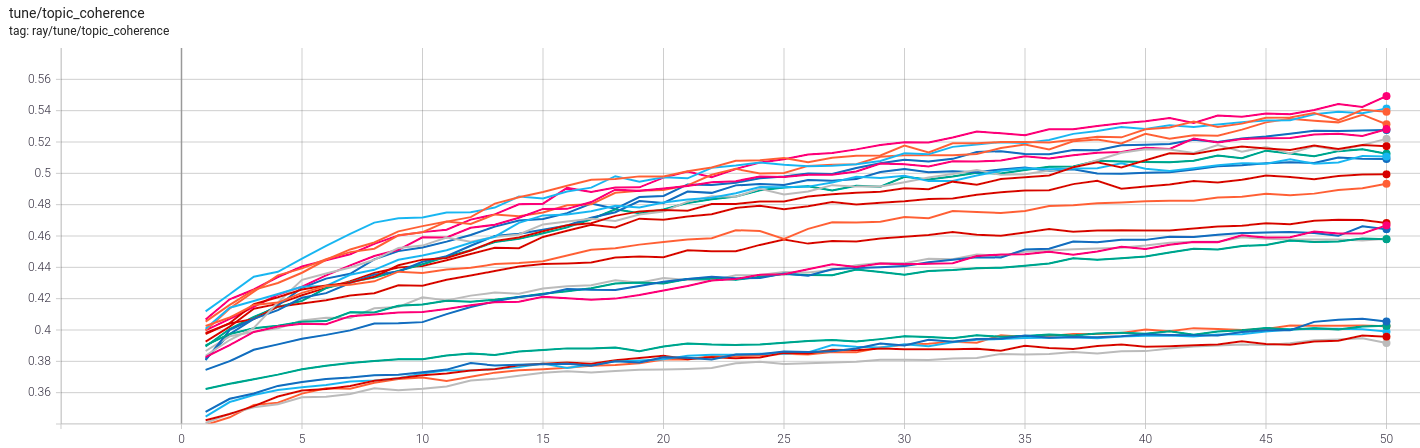
\includegraphics[width=\textwidth]{figures/gridsearch.png}
	\caption{Grid search over the variables in \autoref{tab:gridsearch} $K_2$.}
	\label{fig:visual_grid}
\end{figure} 
The five lowest values in \autoref{fig:visual_grid}, are where the $\alpha$ is $0.1$ and $\beta$ is $0.01$. 
This shows us that having the $\alpha$ high and the $\beta$ low does not yield good coherence results.
The next five values are where the $\alpha$ and $\beta$ is $0.01$, which also shows that a low value in both hyperparameters does not yield the best results either.
There is only a minor difference between the top configurations in \autoref{fig:visual_grid}, but the top two configurations are $70$ and $90$ topics, where $90$ performs best.

\subsection{Coloring articles}\label{app:color_articles}
In this section, we analyze a few more articles to get a more in-depth view of how the topic distributions differ between the models.
We are still looking at the top three topics for each model and taking the 200 most probable words.

As a reminder, the color scheme is shown below in \autoref{tab:appendix_disc_color}.
\begin{table}[h]
	\centering
	\caption{Color scheme for each model.}
	\begin{tabular}{l|c}
		Topic Model & Color \\
		\midrule
		\Acrlong{lda} & \thiscolor{Goldenrod} \vspace*{2mm} \\
		Author-topic model & \thiscolor{Aquamarine} \vspace*{2mm} \\
		Category-topic model & \thiscolor{LimeGreen} \vspace*{2mm} \\
		Taxonomy-topic model & \thiscolor{Orchid} \vspace*{2mm} \\
		Word appearing in 3+ models & \thiscolor{Peach} \vspace*{2mm} \\
	\end{tabular}
	\label{tab:appendix_disc_color}
\end{table}
\noindent
\autoref{art:1} shows an article about a race car driver from Aalborg, and him driving in the European Le Mans Series.
The article is not that long, and therefore there are not many words marked.
From the colored words in the article, the words appearing in all models are not very descriptive of what the article is about.
The topic that is the most present in this article is most likely a sports topic based on the top 10 words.
The top 10 words of this most present \gls{lda} topic are: ['tour', 'vandt', 'løb', 'par', 'mig', 'løbet', 'hold', 'vm', 'slag', 'nummer'].
We can see based on these words that other sports are higher up in the list, such as 'tour' from Tour de France, which is likely due to there being few Le Mans articles in the dataset.
\\
\begin{figure}
	\begin{tcolorbox}
		\emph{
			dårligt \colorbox{Peach}{løb} for aalborg-kører spielberg: den aalborgensiske racerkører anders fjordbach havde sammen med teamet high class racing en gennemført skidt \colorbox{Peach}{tredje} afdeling af \mycolor{Orchid}{Goldenrod}{european} le mans series på red bull ring i østrig. her blev det til en beskeden ottendeplads i lmp2-klassen. - det var \colorbox{Peach}{selvfølgelig} ærgerligt kun at blive \mycolor{Orchid}{Goldenrod}{nummer} otte, men det er \colorbox{LimeGreen}{vel} ikke en skam at have en dårlig weekend, siger anders fjordbach, der \mycolor{Orchid}{Goldenrod}{kører} sammen med \colorbox{LimeGreen}{dennis} andersen.  \colorbox{LimeGreen}{forkert} dækvalg, et \colorbox{Peach}{mindre} sammenstød, en generator, der \mycolor{Orchid}{Aquamarine}{stod} af og andre små problemer var årsagen. det \colorbox{Peach}{eneste} positive var, at teamet \colorbox{Peach}{fortsat} er på tredjepladsen sammenlagt.clajen
		}
	\end{tcolorbox}
	\caption{An article about a race car driver from Aalborg, and him driving in the European Le Mans Series.}
	\label{art:1}
\end{figure}

\autoref{art:2} is about politics in Aalborg, specifically about charter ships docking in Aalborg and how the municipality is trying to solve this problem.
\autoref{art:2} is a bit longer than the one in \autoref{art:1}, which in turn colors more words.
We can see that the majority of these words appear in every model, where a lot of non-descriptive words occur, such as 'finde' (to find), 'giver' (give), and 'ting' (stuff). 
Opposite to the original article analyzed in the paper, word combinations of the category-Topic model and \gls{lda} model are more present within this article.
From the top words within the category-topic model, many generic words appear, which might be why there is a higher trend in word appearances.
The author-topic model is not showing up with many unique words, but the author (Pernille K. Damsgaard) has written $922$ articles, which might indicate that she usually does not write about this topic.
\\
\begin{figure}
	\begin{tcolorbox}
		\emph{
			rådmand: der skal \colorbox{Peach}{findes}  en \mycolor{Orchid}{Goldenrod}{løsning} aalborg: rådmand \colorbox{Peach}{hans} \colorbox{Peach}{henrik} \colorbox{Peach}{henriksen} (s) er indstillet på, at der fra \mycolor{Goldenrod}{LimeGreen}{kommunens} side bidrages til en løsning, der sikrer krydstogtgæsterne sikker adgang på tværs af slotspladsen. - \colorbox{Goldenrod}{lad} os prøve at se, om vi ikke ved \mycolor{Goldenrod}{LimeGreen}{fælles} \colorbox{Peach}{hjælp} kan \colorbox{Peach}{finde} en god løsning, der fungerer, på det her, siger by- og landskabsrådmanden med henvisning til dagsordenen for det \colorbox{Peach}{kommende} \colorbox{Peach}{møde} med deltagelse af visitaalborg, \colorbox{Peach}{kommunen} ved \mycolor{Orchid}{Goldenrod}{trafik} og veje, \mycolor{LimeGreen}{Aquamarine}{politiet} \colorbox{Peach}{samt} aalborg havn, der også har en \mycolor{Goldenrod}{Aquamarine}{interesse} i \mycolor{Goldenrod}{LimeGreen}{udvikling} af krydstogtforretningen. forud for mødet har han ikke noget bud på en løsning, og han gentager en tidligere afvisning af et traditionelt fodgængerfelt. - \colorbox{Peach}{folk} med viden på det felt har forklaret mig, at der \colorbox{Peach}{faktisk} \colorbox{Peach}{sker} flere ulykker i et fodgængerfelt, fordi nogle bilister overser striberne, hvorved det \colorbox{Peach}{giver} gående en falsk tryghed. men \colorbox{Goldenrod}{lad} os nu slette tavlen og se på det med friske øjne, siger rådmanden, der er enig med visitaalborgs \colorbox{Peach}{lars} bech i, at der skal \colorbox{Peach}{findes} en tilfreds stillende løsning. - når vi markedsfører os i \colorbox{Peach}{forhold} til krydstogtsturismen, og ved fra visitaalborg, at det ikke er ligetil at få rederierne til at vælge aalborg, skal der også være en service, der virkelig fungerer, og der \colorbox{Aquamarine}{tæller} de små \colorbox{Peach}{ting} som adgang til \colorbox{Peach}{byen} også. så det her skal vi \colorbox{Peach}{finde} en \mycolor{Orchid}{Goldenrod}{løsning} på. det ville ikke være til at bære, hvis der \mycolor{LimeGreen}{Aquamarine}{skete} en ulykke, siger rådmanden, der mener, at det på tværs vil være \colorbox{Peach}{muligt} at \colorbox{Peach}{finde} de nødvendige \colorbox{Peach}{penge} til et eventuelt nyanlæg, siger rådmanden, der kan forestille sig, at en \colorbox{Peach}{form} for lysregulering kommer til at indgå i løsningen. - det vil ikke være tilstrækkeligt bare at male zebrastriber på vejen, siger han.
		}
	\end{tcolorbox}
	\caption{An article about politics in Aalborg, specifically about charter ships docking in Aalborg and how the municipality is trying to solve this problem.}
	\label{art:2}
\end{figure}
 


% New experiments and related details
\subsection{Stemming the dataset}\label{sec:stemming}
\vejleder{Se dokument for flere kommentarer}
In this project, we have done minimal preprocessing \vejleder{hvad med stop ord, fylde ord?}of the dataset, because, in a previous project, a more aggressive preprocessing step turned out to hurt the performance of the \gls{lda} model.
This made us completely avoid trying to include a stemming process, even though this was only a smaller part of this previous preprocessing step.
Though, after further consideration, it is worth looking into what effect adding just stemming to our current preprocessing, described in \autoref{sec:dataset}, would have on the standard \gls{lda} model.

With stemming included, the number of unique words goes down to $60,651$ from the previous $69,192$ unique words.
This means that 8541 unique words have been stemmed down to their root forms.
Even though much fewer unique words are in our dataset, which can have an effect on which articles are removed, the dataset only goes from $139,064$ articles to $139,060$, which is a removal of 4 articles.

In the non-stemmed \gls{lda} model, words that have no meaning topically seem to have a large influence.
This is still the case in the stemmed model, where words like 'du' (you), 'mig' (me), and 'a' still appear in the top words of topics.
To remove these words, we would have to include some more advanced preprocessing in the form of stop word removal and part-of-speech (POS) tagging.

Examples of top words for similar topics between the models can be seen in \autoref{tab:topic_examples}.
It is seen here that some of the topics between the models are clearly about the same subjects.
The stemmed model's topics might also be slightly more understandable because words with the same meaning (e.g. 'politi' and 'politiet') do not appear.
Other than this, including stemming, does not seem to have made a significant difference.

\begin{table}
	\caption{An example of topics that are similar between the non-stemmed and stemmed \gls{lda} model.
		Here the topics are all about crime and the police.}
	\label{tab:topic_examples}
	\centering
	\begin{tabular}{c|c}
		Model & Topics \\
		\midrule
		\multirow{6}{*}{Non-stemmed} & dræbt, mennesker, personer, politiet, mindst, angreb, oplyser, afp, reuters, byen  \\
		 & stjalet, indbrud, klokken, nordjyllands, thisted, politi, politiet, mandag, villa, oplyser  \\
		 & arige, politiet, mand, arig, politi, sagen, oplyser, indbrud, retten, stjalet  \\
		 & politiet, mand, arig, politi, arige, bil, nordjyllands, thisted, bilen, klokken  \\
		 & arig, bil, mand, politiet, kørte, hobro, bilen, thisted, klokken, arige  \\
		 & arige, politiet, mand, arig, politi, retten, sagen, fængsel, ham, oplyser  \\
		\midrule
		\multirow{5}{*}{Stemmed} & stjal, indbrud, politi, tyv, klok, nordjylland, bil, thisted, tyveri, villa  \\
		 & politi, nordjylland, brand, bil, mand, indbrud, stjal, klok, hus, beredskab  \\
		 & sag, dom, blokhus, advokat, ham, fængsel, sagen, dreng, politi, mand  \\
		 & politi, mand, kvind, sag, sigt, bil, mænd, nordjylland, oplys, anhold  \\
		 & politi, mand, bil, person, oplys, kørt, kvind, sigt, nordjylland, dræbt  \\
	\end{tabular}
\end{table}

%% Code
\subsection{Pyro model implementation}
%XTried different approaches, one being probabilistic programming languages. Pyro
%XBasics behind Pyro (uses SVI for instance)
%Implemented a basic version first
%Expanded their ProdLDA example with metadata information
%Switched to Gibbs sampling to have opportunities to change things in detail
After we decided to work with metadata in \gls{lda} models, we had to firstly get a standard model implemented.
Here we decided to look in a few directions for the best way to implement a generative model, and we found that the probabilistic programming language Pyro could be used.
Pyro is a probabilistic programming language that is written in Python with PyTorch as a backend.
This makes it ideal for making quick implementations of models, with the possibility of using tensors and sampling with PyTorch distribution methods.
Pyro also has a built-in stochastic variational inference class that simplifies the training of a model.
These features made it an ideal programming language to look into.


\subsection{Gibbs sampling}\label{sec:appendix_gibbs}
The Gibbs Sampling algorithm consists of two procedures: Random Initialization and Gibbs Sampling.
In the following sections, we explain how these procedures have been implemented.

\subsubsection{Random Initialization}
Before a Gibbs sampling algorithm can run, every word needs to be assigned a random topic.
To do this, we iterate over each word within each document and assign a random topic to it.
This procedure is shown in \autoref{lst:randomInit}.
\begin{lstlisting}[language=Python, caption=Random Initialization,label={lst:randomInit}, float, floatplacement=H]
import numpy as np

def rand_initialize(documents: List[np.ndarray]):
	wt_assignment = []
	for doc in documents:
		curr_doc = []
		for word in doc:
			# Construct the topic distribution
			pz = _conditional_distribution()
			
			# Draw a new topic and assign it
			t = np.random.multinomial(1, pz).argmax()
			curr_doc.append(t)
			
			# Increase the topic counts
			increase_count()
		wt_assignment.append(curr_doc)
	return wt_assignment
\end{lstlisting}
Various parameters are left out to simplify the code listing of our initialization method.
The \emph{\_conditional\_distribution()} function creates a distribution of topics based on the current word.
Standard \gls{lda} is based on \autoref{eq:gibbs_eq}~\cite{author_topic_2012} and the author-topic and category-topic models are based on \autoref{eq:author_gibbs_eq} and \autoref{eq:category_gibbs_eq}, respectively.
\begin{equation}\label{eq:gibbs_eq}
	\begin{split}
		P(z_i = k|w_i = m, \boldsymbol{z}_{-i}, \boldsymbol{w}_{-i}) \propto 
		\underbrace{\frac{C^{DT}_{dk} + \alpha}{\sum_{k'} C^{DT}_{dk'} + T\alpha}}_{Doc-Topic}
		\underbrace{\frac{C^{WT}_{mk} + \eta}{\sum_{m'} C^{WT}_{m'k} + V\eta}}_{Topic-Word}
	\end{split}
\end{equation}
\begin{equation}\label{eq:author_gibbs_eq}
	\begin{split}
		P(z_i = k|w_i = m, \boldsymbol{z}_{-i}, \boldsymbol{w}_{-i}, a_d) \propto 
		\underbrace{\frac{C^{AT}_{ak} + \alpha}{\sum_{k'} C^{AT}_{ak'} + T\alpha}}_{Author-Topic}
		\underbrace{\frac{C^{WT}_{mk} + \eta}{\sum_{m'} C^{WT}_{m'k} + V\eta}}_{Topic-Word}
	\end{split}
\end{equation}
\begin{equation}\label{eq:category_gibbs_eq}
	\begin{split}
		P(z_i = k|w_i = m, \boldsymbol{z}_{-i}, \boldsymbol{w}_{-i}, c_d) \propto 
		\underbrace{\frac{C^{CT}_{ck} + \alpha}{\sum_{k'} C^{CT}_{ck'} + T\alpha}}_{Category-Topic}
		\underbrace{\frac{C^{WT}_{mk} + \eta}{\sum_{m'} C^{WT}_{m'k} + V\eta}}_{Topic-Word}
	\end{split}
\end{equation}
where $C^{DT}_{dk}$ is the number of times document $d$ uses topic $k$ and $C^{WT}_{mk}$ is the number of times topic $k$ uses word $m$.
$C^{AT}_{ak}$ and $C^{CT}_{ck}$ is the number of times author $a$ and category $c$ use topic $k$, respectively.
$\boldsymbol{z}_{-i}$ represents the topic assignments where the current instance is disregarded.
$\alpha$ and $\eta$ are the Dirichlet parameters for the document-topic and topic-word distribution, respectively.
The first fraction describes how likely topic $t$ appearing in document $d$ is, and the second fraction describes which words are most probable in topic $t$.
Following the code in \autoref{lst:randomInit}, as we initialize, the words get a higher probability of clustering together, since we increase the counts every time at line $16$.
In the author-topic and category-topic models a metadata distribution is used where they follow the functions described in 



\subsubsection{Gibbs Sampling}
We can start investigating the Gibbs sampling method itself, where we iterate over each word in every document and draw a new topic based on the given topic distribution.
As in \autoref{lst:randomInit}, the code has been simplified.
\begin{lstlisting}[language=Python, caption=Gibbs Sampling Method,label={lst:gibbsSampling}, float, floatplacement=H]
import numpy as np

def gibbs_sampling(documents: List[np.ndarray],
	   doc_topic_dist: np.ndarray,
	   doc_topic_count: np.ndarray,
	   topic_word_dist: np.ndarray,
	   topic_word_count: np.ndarray,
	   wt_assignment: List[List[int]]):

	for d_index, doc in documents:
		for w_index, word in enumerate(doc):
			# Get the topic of the current word
			topic = wt_assignment[d_index][w_index]
			
			# Decrease the topic count
			decrease_count()
			
			# Sample a new topic
			pz = _conditional_distribution()
			topic = np.random.multinomial(1, pz).argmax()
			
			# Assign topic to the current word
			wt_assignment[d_index][w_index] = topic
			
			# And increase the topic count
			increase_count()
\end{lstlisting}
The Gibbs sampling method is very similar to the random initialization method in \autoref{lst:randomInit}, but with a few additions. 
Now we introduce the \emph{decrease\_count()} which decreases the topic count for both words and documents, and  \emph{increase\_count()} which increases them.
This is done because new samples need to be calculated based on all other word topic assignments (not including the current word).
The sampling is explained in \autoref{lst:gibbsSampling}.
On line 13, we get the current topic for the given word and on line 23 we assign a newly drawn topic to that word.

\subsection{Parallel Gibbs Sampling}\label{sec:appendix_para_gibbs}
We have also implemented a Gibbs sampler, which works in parallel by splitting up the dataset into $p$ parts, where $p$ is the number of processes.
This is to create $\frac{1}{p}$ amount of progress for each process and then combine them.
Each process gets a specific split of the dataset and the available words. 
This is done to avoid race conditions on increasing and decreasing counts in the Gibbs sampler, which is explained in \autoref{sec:appendix_gibbs}.
However, normally the implementation of this algorithm is run on the GPU, where we implemented it for CPU where IO was very slow.
Because of the slow combination, due to IO, it did not give us any speed up, so the implementation was not used for this project. 

\subsection{Pachinko implementation}
We have implemented a \acrfull{pam} algorithm able to support any \gls{dag} structure, where each layer only has edges to all the nodes in the next layer, as with the 'Four-Level \gls{pam}' presented by \citet{li2006pachinko}.

We use Gibbs sampling for performing inference.
For each word, a chain of topics is sampled by calculating the probability of all combinations of topics and making a weighted sample.
The probability of each topic combination is calculated using the joint probability of the topics, as presented in \autoref{eq:pachinko_gibbs}. This equation is for the 'Five-Level \gls{pam}' that we use in the paper.

\begin{equation}\label{eq:pachinko_gibbs}
	\begin{split}
		P(Z_{w2} = t_a, Z_{w3} = t_b, Z_{w4} = t_c | \textbf{D}, z_{-w}, \alpha, \beta) \propto \\
		\frac{n_{1a}^d + \alpha_{1a}}{n_1^d + \sum_{a'} \alpha_{1a'}} \times
		\frac{n_{ab}^d + \alpha_{ab}}{n_a^d + \sum_{b'} \alpha_{ab'}}  \times 
		\frac{n_{bc}^d + \alpha_{bc}}{n_{b}^d + \sum_{c'} \alpha_{bc'}} \times 
		\frac{n_{cw} + \eta_{w}}{n_{c} + \sum_{m} \eta_{m}} 
	\end{split}
\end{equation}
As in \citet{li2006pachinko}, $Z_{w2}$, $Z_{w3}$, and $Z_{w4}$ are topic assignments for the three middle layers of topics in our Five-Level \gls{pam}.
The root topic is not part of this equation since all words are part of it, so the probability does not need to be calculated.
$Z_{-w}$ is the word topic assignment, for all other words except the one that is being updated.
$n_x^d$ is the number of times topic $t_x$ occurs in document $d$ according to $Z_{-w}$. 
The $n_{xy}^d$ describes how many times topic $t_y$ is sampled from its parent $t_x$ within document $d$ according to $Z_{-w}$.
$n_x$ is the number of times topic $t_x$ occurs in the corpus according to $Z_{-w}$, and $n_{xw}$ is the number of times a word $w$ is in $t_x$ according to $Z_{-w}$.

However, the \gls{pam} framework can support any number of layers using this structure.
In order to do this, we must generalize the process of Gibbs sampling for pachinko using 'level' \gls{dag} structures.
Firstly, before the Gibbs sampling begins a one-time random initialization is made, where each word in each document is randomly assigned to a chain of topics (one for each layer).
In our \gls{pam}, some topic layers represent taxonomy layers, since some documents in the dataset already have a topic entry.
These documents are assigned the topics corresponding to their taxonomy entries, and the rest of the taxonomy chain will then be randomly generated if it is not already complete.

The Gibbs sampling for \gls{pam} consists of the following steps for each word in each document:

\begin{enumerate}
	\item Decrease count
	\item Calculate layer combinations
	\item Multiply layer combinations
	\item Weighted sample
	\item Increase count
\end{enumerate}

Following is an overview of each of the steps.
Firstly, the current word is removed from the counts of how many words are assigned to each topic.
After the count has been decreased, we calculate for each combination of successive layers, the probability of each possible topic combination.
This process will be explained further in \autoref{app:calculate_layer_combs}.

Each of these calculations is combined to calculate the final probability of each possible topic combination.
This process is explained in \autoref{app:multiply_layer_combs}.
One topic combination is then sampled, using a weighted sampling based on the probabilities of all topic combinations.
Finally, once a new topic combination has been chosen, the counts of how many words are assigned to each topic are increased accordingly.

We will now go into more detail about calculating layer combinations and multiplying layer combinations, as these are the main differences between how \gls{lda} and \gls{pam} use Gibbs sampling.
\subsubsection{Calculate layer combinations}\label{app:calculate_layer_combs}
This is done based on observations in \autoref{eq:pachinko_gibbs}.
The equation consist of several fractions equal to the number of layers - 1, with each fraction representing the relationship between two layers.
The last fraction is a little different as it takes word topic assignments for the whole corpus into account, unlike the other fractions which only look at the word topic assignments for the current document.

In order to run efficiently, we calculate all topic combinations at the same time, rather than calculating a specific one as outlined in \autoref{eq:pachinko_gibbs}.
To do this, we operate on vectors and matrices rather than single values.
So for the fraction $\frac{n_{ab}^d + \alpha_{ab}}{n_a^d + \sum_{b'} \alpha_{ab'}}$ from \autoref{eq:pachinko_gibbs}, $n_{ab}^d$ is a matrix which indicates the number of words in document $d$ that has been assigned to each combination of topics in layer $a$ and layer $b$, with one row for each topic in layer $a$ and one column for each topic in layer $b$.
Similarly, $n_a^d$ is a vector showing the number of words in document $d$ assigned to each topic in layer $a$, rather than a single topic.
If some taxonomy entries for the document are already known, the matrices and vectors are sliced to only include the relevant unknown topics.

\subsubsection{Multiplying layer combinations}\label{app:multiply_layer_combs}
Once all the two-layer combinations have been calculated, they have to be combined to find the probability of all topic combinations.
To do so, the layer combinations are multiplied across the dimensions they share.
So for an $A\times B$ matrix and a $B\times C$ matrix, values that share the same $B$ entry are multiplied together to form a three-dimensional $A\times B\times C$ array.
Importantly, the shared dimension is kept, unlike with matrix multiplication.
By keeping all dimensions, the final array will have one entry for all possible topic combinations.

\subsection{Locking the gibbs sampler}\label{sec:appendix/locking}
Normally when working with topic modeling, one does not know which topics will be present in the document set before training the model.
However, the taxonomy metadata fields provides some general subject names of different levels of abstraction and some amount of documents attached to these subject names.
This provides a unique opportunity for using the existing taxonomies as higher-level topics.

The pachinko model normally samples, like the Gibbs sampler, each taxonomy level and estimates the different topics for each document.

However, in our case, we have a partially observed taxonomy and we want to use the existing meta-information to estimate the topics quicker and more accurately.
When we sample in the \gls{pam}, we only sample the unobserved taxonomies and let the observed taxonomies be. 
This has the effect of letting the unobserved taxonomy fit the existing topics within the model and making the process of sampling faster.
However, locking these taxonomies into places also hinders further improvement to the observed taxonomies, since they do not change during training.   

\subsection{Pachinko Results}\label{app:pachinko_res}

\autoref{tab:pachinko_topics} shows the final lowest level topics of the pachinko model.
Note that while most of the topics are semantically coherent, there are a some topics (eg. topic 19 and 42) which consist entirely of words which provide little context or semantic meaning.
The model has also learned to group words that do not belong into any good topics.
This is a good feature which allows the model to apply an extra layer of preprocessing, automatically filtering away irrellevant words into topics.

\begin{longtable}[c]{c | c}
		\caption{Top 10 words for each lowest level topic in the results of the pachinko model \label{tab:pachinko_topics}}\\
		Topic & Top 10 words \\
		\hline
		\endfirsthead
		1 & nordjylland, læger, patienter, region, læge, regionen, praktiserende, sygehus, patienterne, behandling \\
		2 & turister, ferie, lokale, gæster, øen, skagen, strand, byen, steder, ligger \\
		3 & hvordan, unge, fokus, mennesker, skabe, verden, vigtigt, made, handler, hinanden \\
		4 & gamle, maske, ganske, altsa, først, faktisk, forsvaret, næsten, mest, set \\
		5 & direktør, fly, lufthavn, københavn, selskabet, passagerer, thomas, søren, sas, aarhus \\
		6 & mal, halvleg, minutter, kampen, serie, kamp, mors, fc, morsø, thisted \\
		7 & hobro, lørdag, kaffe, jul, mariager, gamle, klokken, december, børn, mulighed \\
		8 & venstre, valg, valget, partiet, partier, parti, stemmer, mette, politik, regering \\
		9 & procent, viser, tal, antallet, milliarder, pct, seneste, penge, millioner, indland \\
		10 & arige, mand, arig, retten, politiet, ham, mænd, fængsel, manden, sagen \\
		11 & virksomheder, nordjylland, nordjyske, virksomhederne, arbejdspladser, samarbejde, arbejdskraft, udvikling, job, vækst \\
		12 & hjørring, teater, vendsyssel, forestillingen, kl, løkken, publikum, lørdag, klokken, festivalen \\
		13 & offentlige, penge, bedre, mener, kommunerne, regeringen, ansatte, kommuner, brug, arbejde \\
		14 & mig, henrik, christensen, ham, hans, andersen, jensen, arbejde, rigtig, synes \\
		15 & arets, prisen, bedste, pris, meter, vandt, dansk, thisted, guld, nordjyske \\
		16 & salg, gamle, peter, sælge, solgt, firmaet, købe, ejer, niels, sat \\
		17 & brand, branden, beredskab, gik, kvinder, huset, nordjyllands, ilden, matte, ild \\
		18 & foredrag, bøger, bibliotek, bogen, bog, biblioteket, forfatter, foredraget, historie, dk \\
		19 & mig, maske, du, folk, synes, ting, faktisk, nogen, altid, tror \\
		20 & syrien, dræbt, tyrkiet, fn, angreb, al, mennesker, israel, stat, islamisk \\
		21 & unge, uddannelse, studerende, gymnasium, elever, uddannelser, universitet, procent, uddannelsen, nordjylland \\
		22 & havn, havnen, hanstholm, fisk, skagen, hirtshals, meter, vandet, skibe, skibet \\
		23 & nielsen, løb, nummer, vm, jakobsen, formel, dm, banen, skelund, løbet \\
		24 & grader, vejr, varme, sommer, regn, vejret, dage, vand, landet, uge \\
		25 & aab, jacob, kasper, rasmus, jakob, pedersen, andersen, friis, minut, allan \\
		26 & tyske, døde, hans, børn, skriver, personer, politiet, mennesker, tyskland, død \\
		27 & klubben, hold, medlemmer, unge, sport, fodbold, u, klub, cup, træning \\
		28 & børn, skole, børnene, forældre, skolen, elever, forældrene, unge, barn, voksne \\
		29 & vm, league, klubben, spiller, fodbold, spillere, kampe, manchester, em, champions \\
		30 & sagen, fængsel, retten, sag, arige, dom, dømt, dommen, ars, idømt \\
		31 & arbejde, arbejdsmarkedet, pension, job, grønland, ret, f, personer, nedslidte, folk \\
		32 & dette, politikere, maske, mig, vel, disse, mennesker, hvorfor, nogen, land \\
		33 & frederikshavn, millioner, svenske, sverige, norge, milliarder, norske, procent, dollar, solgt \\
		34 & hobro, hadsund, morgen, mariagerfjord, bio, sker, rebild, øster, arr, skørping \\
		35 & gamle, museum, naturen, omradet, natur, skov, ligger, lille, projektet, historiske \\
		36 & formand, jensen, nielsen, jens, erik, jørgen, sørensen, bestyrelsen, pedersen, sagde \\
		37 & køre, trafik, trafikken, kører, biler, vejen, vej, egholm, motorvej, forbindelse \\
		38 & lars, f, arbejde, dansk, formand, medlemmer, ansatte, rasmussen, leder, mig \\
		39 & kommunen, sagen, mener, kommunens, sag, hjørring, kystsikring, teknik, omradet, sager \\
		40 & hans, film, ham, filmen, anders, tv, erne, fylder, skuespiller, liv \\
		41 & universitet, professor, forskere, forskning, forskerne, viser, verden, institut, procent, aarhus \\
		42 & mig, min, mit, ham, aldrig, gik, lille, maske, mine, altid \\
		43 & fc, point, aab, kampe, kamp, hold, brøndby, holdet, vendsyssel, mal \\
		44 & aars, vesthimmerland, brønderslev, løgstør, vesthimmerlands, farsø, børn, frivillige, dronninglund, kors \\
		45 & dyr, naturen, natur, ulve, fugle, ulven, arter, dyrene, vilde, ulv \\
		46 & bank, banken, millioner, nordjyske, banks, penge, ebh, jyske, kunder, bankens \\
		47 & kirke, kirken, sognepræst, præst, søndag, koret, gudstjeneste, aften, kor, organist \\
		48 & sagen, skriver, fejl, oplysninger, sag, politiet, reglerne, mener, indland, kontrol \\
		49 & eu, europa, lande, europæiske, tyskland, kommissionen, parlamentet, tyske, bruxelles, polen \\
		50 & usa, trump, amerikanske, new, præsident, york, donald, washington, skriver, hus \\
		51 & jammerbugt, brønderslev, projektet, aabybro, nyt, plads, klar, kvadratmeter, byen, brovst \\
		52 & usa, præsident, trump, kina, rusland, amerikanske, russiske, iran, reuters, sagde \\
		53 & du, facebook, digitale, medier, it, data, dk, bruger, via, nettet \\
		54 & borgmester, kommuner, v, sagde, byradet, nordjyske, mogens, borgmesteren, arne, per \\
		55 & biler, bil, model, bilen, modeller, a, vw, e, ford, toyota \\
		56 & mad, vin, øl, restaurant, spise, smag, kød, maden, hund, spiser \\
		57 & vandt, runde, slag, par, vm, turneringen, wozniacki, nummer, open, sæt \\
		58 & kr, mio, morsø, kommunen, penge, mors, millioner, rebild, budget, tilskud \\
		59 & musik, koncert, sange, spiller, koncerter, band, koncerten, festival, musikken, publikum \\
		60 & virksomheden, millioner, a, direktør, procent, medarbejdere, selskabet, overskud, ansatte, virksomhed \\
		61 & minut, hobro, mal, kamp, mikkel, vendsyssel, kampen, frederikshavn, pirates, kampe \\
		62 & støvring, tog, skagen, rebild, dsb, nordjyske, trafik, køre, nordjylland, kører \\
		63 & arig, mand, bil, politiet, kørte, politi, bilen, arige, skete, klokken \\
		64 & sygdom, behandling, mennesker, patienter, medicin, parørende, sygdommen, syge, sundhed, psykisk \\
		65 & boliger, omradet, kommunen, lokalplan, projektet, byggeri, møller, vindmøller, teknik, omrade \\
		66 & tv, the, film, of, dr, filmen, serien, fem, a, hver \\
		67 & energi, el, grøn, grønne, procent, co, omstilling, strøm, varme, kr \\
		68 & butikken, butikker, butik, sæby, kunder, kunderne, nykøbing, varer, købmand, mors \\
		69 & elever, unge, skole, eleverne, skolen, skoler, klasse, børn, folkeskolen, lærere \\
		70 & unge, politiet, kvinder, antallet, mænd, borgere, politi, vold, personer, udsatte \\
		71 & plads, byen, p, hotel, by, gamle, byens, pladser, omradet, hus \\
		72 & politiet, politi, indbrud, mand, stjalet, nordjyllands, klokken, arig, oplyser, thisted \\
		73 & du, jorden, haven, planter, vand, ned, træer, blomster, sma, jord \\
		74 & ældre, borgere, kommunen, millioner, penge, nordjylland, plejehjem, borgerne, kommunens, budget \\
		75 & du, din, dig, dit, altsa, dine, maske, nemlig, bruge, hvordan \\
		76 & tour, etape, løbet, kilometer, michael, fuglsang, nord, france, hold, spar \\
		77 & regeringen, penge, bedre, samfund, mennesker, dette, disse, børn, dansk, sikre \\
		78 & kunst, udstillingen, udstilling, værker, kunstnere, museum, malerier, kunstner, billeder, kunsten \\
		79 & mig, min, hendes, hende, rigtig, arige, altid, arbejde, mor, mine \\
		80 & km, kr, hk, t, m, bilen, motor, a, bil, l \\
		81 & stjalet, indbrud, mandag, madsen, klokken, kl, politiet, tirsdag, onsdag, thisted \\
		82 & dansk, regeringen, løkke, v, venstre, lars, folkeparti, df, rasmussen, mener \\
		83 & ord, bogen, bog, liv, verden, skrevet, hendes, du, historie, skriver \\
		84 & løbet, rebild, blokhus, løb, deltagerne, deltagere, turen, kl, kilometer, tur \\
		85 & thisted, thy, mors, hanstholm, klitmøller, vorupør, hurup, lokale, nationalpark, morsø \\
		86 & handbold, mors, thy, hold, kamp, sæson, kampe, kampen, point, holdet \\
		87 & prins, fylder, henrik, hans, larsen, tv, kim, københavn, senere, født \\
		88 & eu, britiske, brexit, storbritannien, aftale, london, may, premierminister, johnson, theresa \\
		89 & frivillige, foreningen, løgstør, aktiviteter, lokale, foreninger, medlemmer, forening, formand, lørdag \\
		90 & landbrug, landbruget, landmænd, vand, miljø, affald, bedre, natur, vandløb, fødevarer \\
\end{longtable}

\autoref{tab:pachinko_mid_topics} gives an overview of how the taxonomy topics in the third layer of the pachinko model, are connected to the fourth layer topics that were generated by the model.
Some of these connections make a lot of sense, such as the 'Økonomi' (Economy) topic which has the three filler topics: 79, 75, and 42, which consists of words with little semantic value, and two topics which are about money: 74 and 9.
However not all the connections make as much sense as these. For example the 'Kriminalitet' (Crime) topic has two filler topics: 42 and 75, one topic about economy: 60, one topic about politics: 8, and one topic about sports: 86.
See \autoref{tab:pachinko_topics}, for more details on the top words within each of these topics.

\begin{table}[H]
	\centering
	\caption{Ids of the top 5 most occuring fourth layer topics for each third layer topic from the pachinko model. See table \autoref{tab:pachinko_topics} for most occouring words for each id.}
	\label{tab:pachinko_mid_topics}
	\begin{tabular}{c | c | c | c | c | c}
		Taxonomy Name & Top 5 Topic ids & Taxonomy Name & Top 5 Topic ids & Taxonomy Name & Top 5 Topic ids \\ \hline
		Danmark & 8, 42, 82, 59, 79 & Udland & 42, 79, 59, 8, 32 & Kultur & 9, 42, 79, 19, 8 \\
		Landbrug & 42, 79, 8, 9, 19 & Kriminalitet & 42, 75, 60, 8, 86 & Socialstof & 42, 9, 79, 86, 8 \\
		Arbejdsmarked & 42, 79, 59, 8, 9 & Økonomi & 79, 75, 74, 42, 9 & Sundhed & 8, 32, 42, 9, 19 \\
		Politik & 42, 75, 9, 19, 74 & Musik & 75, 42, 59, 11, 79 & Sport & 42, 75, 8, 59, 52 \\
		Bolig & 75, 42, 86, 79, 8 & Videnskab & 42, 8, 52, 79, 19 & Trafik & 42, 74, 8, 52, 32 \\
		Erhverv & 42, 8, 59, 32, 79 & Uddannelse & 42, 9, 75, 32, 74 & Energi & 42, 8, 79, 19, 86 \\
		Ulykker & 42, 75, 9, 79, 32 & Fritid & 42, 8, 75, 82, 79 & Socialt & 42, 75, 79, 59, 9 \\
		Dyr & 86, 42, 79, 52, 9 & Natur & 42, 52, 9, 32, 79 & Miljø & 8, 42, 75, 52, 59 \\
		Familie & 79, 8, 42, 59, 32 & Politi & 42, 75, 79, 8, 59 & Byggeri & 75, 42, 79, 77, 59 \\
		Etik & 79, 42, 8, 86, 74 & Religion & 42, 79, 8, 59, 32 & Kommunalvalg & 42, 8, 75, 79, 32 \\
		Nordjyske Plus & 42, 86, 9, 79, 74 & DF & 42, 8, 59, 52, 19 & & \\
	\end{tabular}
\end{table} % The big table
%% New models
\subsection{Category and author \gls{pam}}\label{app:cat_auth_pachinko}
Given the good results of the taxonomy-topic model, we decided to test \gls{pam} with the two other metadata types: Author and Category.
These metadata are not layered and can therefore not utilize the layered nature of \gls{pam} in the same way.
Instead, a Four-Level \gls{pam} is used, with a root layer, a metadata layer where authors and categories are locked into topics using the technique outlined in \autoref{subsec:pam}, a layer with 90 'blank' topics, and a word layer.

As can be seen from the results in \autoref{tab:cat_auth_pachinko_results}, these models achieve better results than the previous author and category models and the \gls{lda} model.
However, the taxonomy-topic model is still better overall.
The same conclusion is reached after manual inspection of the topics of these models.

\begin{table}[b]
	\centering
	\caption{Topic coherence of author \gls{pam}, category \gls{pam}, and \gls{pam} without metadata (marked with bold) compared to previous models.}
	\begin{tabular}{l|c}
		Topic Model & \makecell{Topic \\ Coherence} \\
		\midrule
		\Acrlong{lda} & 0.520 \\
		Author-topic model & 0.335 \\
		Category-topic model & 0.370 \\
		Taxonomy-topic model & 0.660 \\
		\textbf{Author \gls{pam}} & \textbf{0.598} \\
		\textbf{Category \gls{pam}} & \textbf{0.585} \\
		\textbf{\Acrlong{pam}} & \textbf{0.670} \\
	\end{tabular}
	\label{tab:cat_auth_pachinko_results}
\end{table}

For comparison we also ran a Four-Level \gls{pam} without any metadata, using 100 and 90 as the sizes of the two middle layers.
This ended up providing very good results, slightly better than the taxonomy-topic model.
The elapsed time of the Four-Level \gls{pam} was ${\sim}128$ hours for $50$ epochs, roughly the same as our Five-Level taxonomy-topic model, which had an elapsed time of $132$ hours for $50$ epochs.
The slower speed compared to the size of the \gls{dag} structure is due to this model being unable to skip observed values when sampling since it does not incorporate any metadata.
This also shows that while Category \gls{pam} and Author \gls{pam} get better results than their \gls{lda} counterparts, it is better to run \gls{pam} without modifications.
This could be due to our models being unable to make good use of the extra information provided by the metadata.
It might also point towards these two particular metadata types not being particularly useful in this specific project.
The category metadata is generally very vague and some categories have seemingly no connection between documents.
As discussed earlier, the author metadata might not be as useful within journalism as authors don't write about the same topics as with scientific papers.
And while the \gls{pam} without metadata does achieve better topic coherence than the taxonomy-topic model, they are close enough in both topic coherence and manual inspection of the quality of topics that no conclusions can be drawn.

\subsection{The author-category model}\label{sec:combination}
We have created a combination model, as an extension of our metadata models, to see whether using multiple metadata fields at the same time to draw topics, would affect the performance of the topic model.
The idea is that this model combination should give insight into what a model learns when multiple metadata influence the topics chosen.
The model we have created is the Author-Category combination model.
As the name suggests, this model includes an author-topic distribution and a category-topic distribution, and the plate notation can be seen in \autoref{fig:author_category_lda}.

To combine the author and category metadata, we use the notation described in \citet{author_topic_2012} and in \autoref{sec:appendix_gibbs}.
\begin{equation}
		P(z_i = k |w_i = m, \boldsymbol{z}_{-i}, \boldsymbol{w}_{-i}) = 
	\underbrace{\frac{C^{AT}_{ak} + \alpha}{\sum_{k'} C^{AT}_{ak'} + T\alpha}}_{Author-Topic}
	\underbrace{\frac{C^{CT}_{ck} + \alpha}{\sum_{k'} C^{CT}_{ck'} + T\alpha}}_{Category-Topic}
	\underbrace{\frac{C^{WT}_{mk} + \eta}{\sum_{m'} C^{WT}_{m'k} + V\eta}}_{Topic-Word}
\end{equation}
where $C^{AT}_{ak}$ and $C^{CT}_{ck}$ is the number of times author $a$ and category $c$ use topic $k$, respectively.
The intuition behind this is to multiply the three distributions together to get a combined distribution to draw a topic from.
But before drawing a topic, we normalize it based on the sum of the distribution.
\begin{equation}
	dist = \frac{x}{\sum_{1}^{K} x}
\end{equation}

\begin{figure*}[ht]
	\centering
	\resizebox{.3\textwidth}{!}{%
		\begin{tikzpicture}
	[
	observed/.style={minimum size=26pt,circle,draw=blue!50,fill=blue!20},
	unobserved/.style={minimum size=26pt,circle,draw},
	post/.style={->,>=stealth',semithick},
	]
	
	\node (w-j) [observed] at (0,0) {$W_{d,n}$};
	\node (z-j) [unobserved, above of= w-j, node distance=2.5cm] {$Z_{d,n}$};
	\node (author_obs) [observed, above of= z-j, node distance=2.5cm] {${a_d, c_d}$};
	\node (author_dist) [unobserved, left of=z-j, node distance=2.5cm] {$\theta_a$};
	\node (category_dist) [unobserved, left of=author_obs, node distance=2.5cm] {$\theta_c$};
	\node (alpha-hyper) [unobserved, label=above:$\alpha$, above of=eta-hyper, node distance=3.75cm] {};
	\node (beta-hyper) [unobserved, left of = w-j, node distance=2.5cm] {$\beta_k$};
	\node (eta-hyper) [unobserved, label=above:$\eta$, left of=beta-hyper, node distance=2cm] {};
	
	\path
	(z-j) edge [post] (w-j)
	(alpha-hyper) edge [post] (author_dist)
	(alpha-hyper) edge [post] (category_dist)
	(category_dist) edge [post] (z-j)
	(author_obs) edge [post] (z-j)
	(author_dist) edge [post] (z-j)
	(beta-hyper) edge [post] (w-j)
	(eta-hyper) edge [post] (beta-hyper)
	;
	
	\node [draw,fit=(w-j) (author_obs), inner sep=14pt] (plate-context) {};
	\node [below right] at (plate-context.north west) {$D$};
	
	\node [draw,fit=(w-j) (z-j), inner sep=10pt] (plate-token) {};
	\node [below left] at (plate-token.north east) {$N$};
	
	\node [draw,fit=(beta-hyper) (beta-hyper), inner sep=17pt] (plate-context) {};
	\node [above right] at (plate-context.south west) {$K$};
	
	\node [draw,fit=(author_dist) (author_dist), inner sep=17pt] (plate-context) {};
	\node [above right] at (plate-context.south west) {$A$};
	
	\node [draw,fit=(category_dist) (category_dist), inner sep=17pt] (plate-context) {};
	\node [above right] at (plate-context.south west) {$C$};
	
\end{tikzpicture}
	}
	\caption{Plate notation for the author-category model.}
	\label{fig:author_category_lda}
\end{figure*}

\subsection{Author-category model analysis}
While the results of the models with a single metadata are the most interesting\vejleder[inline]{i hvilken sammenhæng?}, looking at the results of the Author-Category model may also bring new observations.
In \autoref{tab:_extra_metric_results} the metric results for this model is shown, and in \autoref{tab:all_gibbs_topic_examples}, random samples of topics from the \gls{lda}, author-topic, category-topic, and author-category model can be seen.
For the author-category model, the top words in the topics do for the most part not make a lot of sense\vejleder[inline]{uddyb}, though, the author-topic and category-topic models also have topics that are difficult to understand.
It seems, to some degree, that the topics are a mix of the top words of the two combined metadata topic distributions, which makes sense since we draw word topics from a multiplication of these.
While the topics may be less understandable, having a topic distribution for authors and categories gives more opportunities for, e.g., applying these in article recommendation, compared to only having one topic distribution.

\begin{table}
	\caption{A sample of random topics' top 10 words, for the \gls{lda}, author-topic, category-topic, and author-category model. 
	Each section in this table presents 15 random topics, where each topic is randomly picked from the model on the left and each line represents a topic.}
	\label{tab:all_gibbs_topic_examples}
	\centering
	\begin{tabular}{c|c}
		Model & Topics \\
		\midrule
		\multirow{15}{*}{\gls{lda}} & millioner, direktør, sæby, seneste, tv, mener, stadig, landbrug, fokus, bedre \\
		& stjalet, indbrud, klokken, nordjyllands, thisted, politi, politiet, mandag, villa, oplyser \\
		& omradet, boliger, natur, naturen, ligger, du, vand, dyr, a, skov \\
		& du, hans, ham, arige, mig, sagde, stedet, folk, liv, min \\
		& millioner, procent, tv, selskabet, milliarder, skriver, største, aars, direktør, københavn \\
		& thy, thisted, mors, unge, nielsen, arbejde, jensen, a, frederikshavn, folk \\
		& omradet, kommunen, boliger, kr, projektet, byen, a, millioner, by, nyt \\
		& arige, politiet, mand, arig, politi, retten, sagen, fængsel, ham, oplyser \\
		& børn, du, børnene, hvordan, min, mor, forældre, livet, mennesker, skole \\
		& biler, km, bilen, kr, hk, bil, t, a, vw, motor \\
		& hobro, hadsund, mariager, morgen, mariagerfjord, bio, the, sker, kl, filmteatret \\
		& mig, min, hans, liv, altid, du, mennesker, maske, verden, lille \\
		& millioner, bank, sagen, nordjyske, penge, dansk, sag, skat, lars, sagde \\
		& ebh, bank, finn, finansiel, kunst, lørdag, indbrud, vendsyssel, nordjylland, banks \\
		& km, kr, hk, t, bilen, thisted, bil, biler, a, m \\
		\midrule
		\multirow{15}{*}{Author-topic} & du, formand, tale, fem, kr, betyder, dermed, mal, arets, ligger \\
		& jens, ford, vif, london, januar, team, problemerne, eh, vendsyssel, bla \\
		& seneste, bjarne, gruppen, vendsyssel, erik, abent, middelboe, lavendel, nationalpark, motorvejen \\
		& foie, karstensen, elin, bonderup, fredrik, derhjemme, hector, hee, kjøller, lillian \\
		& skriver, hobro, sine, kommuner, dk, jammerbugt, set, min, mig, bedste \\
		& jobi, tilværelse, crowdfunding, klippekortet, knude, nyby, thea, bpa, regi, judo \\
		& du, sine, formand, seneste, jensen, hvert, nyt, hvordan, finde, kommunen \\
		& guaido, fordele, albert, smed, forslag, fie, tørken, krævede, egon, tingene \\
		& rundt, netop, gange, mig, gik, kr, større, landet, universitet, livet \\
		& du, dansk, thisted, mig, procent, eu, ned, arbejde, hans, mener \\
		& mig, millioner, skriver, ham, kommunen, hver, nordjylland, unge, sine, mand \\
		& set, glas, odense, vesthimmerland, leth, markedet, trump, ni, regionerne, prins \\
		& bælum, juul, udlændingenævnet, fruevej, vaarst, svitlana, jernstøberi, bislev, bannere, lo \\
		& carl, resultat, poul, krabbe, p, ansat, begynde, holger, ledelse, g \\
		& ned, procent, arige, eu, made, ham, først, større, mennesker, lyder \\
		\midrule
		\multirow{15}{*}{Category-topic} & foregar, passer, imidlertid, yde, mængder, parlamentet, boris, henvendelser, white, berg \\
		& yderste, sæsonen, lykkes, jernbaner, salgsprisen, efterladt, kakeeto, aab, frygt, rigtigt \\
		& du, børn, mig, hans, unge, procent, mener, politiet, hvordan, thisted \\
		& mener, langt, seneste, ting, mors, give, egen, hurtigt, seks, nej \\
		& du, thisted, dansk, unge, mig, børn, a, hans, procent, arbejde \\
		& jasmin, chelsea, rahbek, norden, partnerskabet, malstregen, eva, modernisering, festligt, byggefirmaet \\
		& nordjyske, hjørring, giver, forhold, hobro, heller, mors, rundt, række, mulighed \\
		& etiske, træningstilbud, lei, statuen, raab, torsdagscafe, aula, pattedyr, berømmelsen, ydet \\
		& omtumlet, sydvendt, gla, dine, golde, trilogi, guidning, jungersen, areal, konservatorer \\
		& nordjyske, sagde, plads, made, dette, fredag, omradet, heller, fald, byen \\
		& sine, hver, skabe, juni, lars, tyskland, vendsyssel, michael, interesse, din \\
		& min, jorden, dit, udfordring, thomas, datter, konkurrence, situation, museum, drive \\
		& the, løbet, stjalet, regering, gaet, tredje, sikkert, byens, omradet, turen \\
		& du, min, gode, gamle, ad, henrik, eu, finde, sat, hobro \\
		& bedre, thy, haft, ham, hver, gik, synes, lars, millioner, eksempel \\
		\midrule
		\multirow{15}{*}{Author-category} & ebh, klare, glas, kvaliteten, finansiel, rebecca, karrieren, storgaard, tørre, børnehave \\
		& du, unge, sagde, samtidig, procent, bedste, hans, brønderslev, hvordan, kommende \\
		& socialdemokratiske, placeres, ellemann, laustsen, fischer, san, regnskabsar, ordentligt, vejgaard, symptomer \\
		& grønland, norden, morris, kenneth, logan, taliban, niki, robinson, tonnies, quinoa \\
		& ganske, største, rød, tyrkiet, tilfældet, dybt, bo, f, fodbold, utrolig \\
		& tror, klar, disse, handler, a, pedersen, holder, mors, borgmester, november \\
		& lola, børnetallet, anklagemyndighed, lagring, madbar, daimler, fortænke, celtic, videnskabsfolk, lokalitet \\
		& reducerede, forældrepar, utrygt, opgøres, pmi, judy, fusk, claude, matine, forsikrings \\
		& egebjerg, overbelægning, gundersen, floden, karrenbauer, involvere, imerco, udviklingsomrader, hh, skygger \\
		& drive, elektrificeres, bryggeriforeningen, fortjenstmedalje, brændstofpriser, sports, afmærket, ball, fanebærer, legal \\
		& velfærdsstat, fortæl, nævneværdigt, solskin, adsbøl, børnesoldater, uvelkomne, reaktioner, daniel, messing \\
		& benn, hadet, knortegas, højskolens, højreradikale, vietnamesere, sner, florence, partiprogram, puk \\
		& du, børn, hans, unge, thisted, hvordan, arige, procent, mand, sagde \\
		& frederiksen, skabt, tæt, halv, sociale, jammerbugt, jørgensen, norge, danskere, ligesom \\
		& skarpere, venskab, landvind, china, motionsform, spørges, drøner, tværfaglige, islændinge, bevæget \\
	\end{tabular}
\end{table}


\subsection{The author-doc and category-doc models}\label{subsec:app_exten_models}
Looking at the results in \autoref{tab:metric_results}, the author-topic and category-topic models do not get very high scores in topic coherence.
In an attempt to improve these results, we combine the original \gls{lda} model with these models, adding a topic distribution for each document and combining it with the existing topic distributions, as with the author-category model, which is explained in \autoref{sec:combination}.
Therefore, we create two extra models: the author-doc and category-doc model.
We run them using the same hyperparameters as all the other models and they get similar results to the standard \gls{lda} model.

The function for choosing a topic is shown for both models in \autoref{eq:doc_author} and \autoref{eq:doc_category}. 
\begin{equation}\label{eq:doc_author}
	P(z_i = k |w_i = m, \boldsymbol{z}_{-i}, \boldsymbol{w}_{-i}) \propto 
	\underbrace{\frac{C^{AT}_{ak} + \alpha}{\sum_{k'} C^{AT}_{ak'} + T\alpha}}_{Author-Topic}
	\underbrace{\frac{C^{DT}_{dk} + \alpha}{\sum_{k'} C^{DT}_{dk'} + T\alpha}}_{Doc-Topic}
	\underbrace{\frac{C^{WT}_{mk} + \eta}{\sum_{m'} C^{WT}_{m'k} + V\eta}}_{Topic-Word}
\end{equation}
where $C^{AT}_{ak}$ and $C^{DT}_{dk}$ is the number of times author $a$ and document $d$ use topic $k$, respectively.

\begin{equation}\label{eq:doc_category}
	P(z_i = k |w_i = m, \boldsymbol{z}_{-i}, \boldsymbol{w}_{-i}) \propto
	\underbrace{\frac{C^{CT}_{ck} + \alpha}{\sum_{k'} C^{CT}_{ck'} + T\alpha}}_{Category-Topic}
	\underbrace{\frac{C^{DT}_{dk} + \alpha}{\sum_{k'} C^{DT}_{dk'} + T\alpha}}_{Doc-Topic}
	\underbrace{\frac{C^{WT}_{mk} + \eta}{\sum_{m'} C^{WT}_{m'k} + V\eta}}_{Topic-Word}
\end{equation}
where $C^{CT}_{ck}$ and $C^{DT}_{dk}$ is the number of times category $c$ and document $d$ use topic $k$, respectively.

\begin{table}[h]
	\centering
	\caption{Results from the combination models: author-category, author-doc, and category-doc (marked with bold) compared to previous models.}
	\begin{tabular}{l|c|c}
		Topic Model & \makecell{Topic \\ Coherence} & \makecell{Topic \\ Difference} \\
		\midrule
		\Acrlong{lda} & 0.520 & 0.575 \\
		Author-topic model & 0.335 & 0.615 \\
		Category-topic model & 0.370 & 0.560 \\
		\textbf{Author-category model} & \textbf{0.390} & \textbf{0.537} \\
		\textbf{Author-doc model} & \textbf{0.543} & \textbf{0.574} \\
		\textbf{Category-doc model} &\textbf{ 0.530} & \textbf{0.575} \\
	\end{tabular}
	\label{tab:_extra_metric_results}
\end{table}

When looking at the topics that the two models produce, and comparing them, we can see some subtle differences, which might indicate the influence of the metadata.
\begin{table}
		\centering
	\caption{Top 10 words for similar topics within the extension models author-doc and category-doc. The topics have been manually selected.}
	\begin{tabular}{l|c|c|c|c|c|c|c|c|c|c}
		Model pairs & 1 & 2 & 3 & 4 & 5 & 6 & 7 & 8 & 9 & 10 \\
		\midrule
		Author-doc & wozniacki & vandt & open & sæt & turneringen & caroline & hobro & runde & nummer & arige \\
		Category-doc & vandt & wozniacki & nummer & runde & open & sæt & turneringen & par & slag & dansk \\
		\midrule
		Author-doc & eu & brexit & britiske & storbritannien & aftale & may & parlamentet & sagde & london & premierminister \\
		Category-doc & eu & brexit & britiske & storbritannien & parlamentet & may & aftale & europa & london & johnson \\
		\midrule
		Author-doc & natur & dyr & landbrug & naturen & landmænd & skov & hektar & vand & lille & danmarks \\
		Category-doc & naturen & natur & du & dansk & hvordan & maske & omradet & landbrug & penge & kystsikring \\
	\end{tabular}
	\label{tab:top_word_comparison}
\end{table}
We have taken 3 topic pairs, which seem to be about the same topics, and compare them between the models.
The first topic pair in \autoref{tab:top_word_comparison} is about tennis since some of the words are talking about Caroline Wozniacki, who is a professional Danish tennis player, and "turneringen" (the tournament).
Specifically, "caroline" is not in the top 10 of the category-doc model which might indicate that the authors have written about "caroline wozniacki" before in other contexts.
The word "slag" (hit) is also used within tennis, which might indicate that the category metadata helps bring sports words higher up in the ranks.
Otherwise, there are no significant differences in the words they use.

Looking at the second pair of topics, which is about the EU and Great Britain, we can see that they are very similar.
The 8th word for the author-topic model is "sagde" (said), which is not a very informative word regarding the topic, but an author might use these kinds of words many times during an article.
Other than that, the topics are very similar when looking at the 10 most probable words.

The third pair of topics is about nature and agriculture.
These two topics are not as similar as the other two pairs we have looked at, but they have two different viewpoints on this topic.
The author-doc model describes words concerning agriculture since two of the words used are "landbrug" (agriculture) and "landmand" (farmer). 
It also mentions nature, with words such as: "natur" (nature), "dyr" (animals), "skov" (forest), and "vand" (water).
The category-doc model describes nature as well but is more focused on areas within nature since the words "området" (the area) and "kystsikring" (coastal protection) are used.
The model might focus more on the debate within the nature topic, which could be about coastal protection.    


% Applications
\subsection{Applications of our models}\label{sec:appendix_applications}
There are a variety of different applications that topic modeling could be used for. 
\citet{Probabilistic_Topic_Models} describes many different purposes for topic modeling, like exploring the history of news articles over time.
The \gls{lda} model, created by \citet{blei2003latent}, has seen many extensions over the years to try and improve the generality of the model.
Normally \gls{lda} works by inferring hidden topic structure, which is based on two distributions, namely the document-topic and topic-word distributions.
An extension to the \gls{lda} is the Author-Topic model, created by \citet{author_topic_2012}, which creates a relationship between the author metadata and the corpus.
This idea of taking metadata into account seems to be overlooked, even though a few papers have touched upon this area, the application possibilities for these kinds of metadata integrations are endless.

News media groups, like Nordjyske, are trying to find new ways of integrating smarter and more intelligent methods for keeping their customers, and using topic modeling could help improve their processes such as searching, recommendation, grouping of articles, and information completion.
We will briefly give an overview of each of these to explain how topic modeling might play a role in improving these processes.

The first example is to improve search functionality for their articles.
This problem could be alleviated by using the topics created by our topic models for performing query expansions finding similar words to the ones that appear in the query, providing more context to find results from.
Once initial search results have been found, topic models could also be used to find other results with similar topics.
These techniques can be particularly useful as they can help find articles that do not use any of the words in a given query but are still relevant to the query, which is a property that most basic search algorithms do not possess.

Another very important problem within news agencies is the recommendation of articles.
Topic models can be used particularly for content-based filtering, finding other articles with similar topic distributions, either based on a user's preferences represented by an interaction history or based on a specific article being read.

Grouping items together, or clustering, can serve many different purposes. 
Topic modeling provides a new way of grouping together articles based on topic similarity.

A topic model might also be used to fill in missing metadata information in an article dataset.
For example, with the taxonomy-topic model, we sample new taxonomies for the majority of the dataset, which does not already have a taxonomy entry.


\end{document}
